% 独自のコマンド

% ■ アブストラクト
%  \begin{jabstract} 〜 \end{jabstract}  :日本語のアブストラクト
%  \begin{eabstract} 〜 \end{eabstract}  :英語のアブストラクト

% ■ 謝辞
%  \begin{acknowledgment} 〜 \end{acknowledgment}

\newif\ifjapanese

\japanesetrue  % 論文全体を日本語で書く(英語で書くならコメントアウト)

\ifjapanese
  \documentclass[a4j,twoside,openright,11pt]{jreport} % 両面印刷の場合。余白を綴じ側に作って右起こし。
  %\documentclass[a4j,11pt]{jreport}                  % 片面印刷の場合。
  \renewcommand{\bibname}{参考文献}
  \newcommand{\acknowledgmentname}{謝辞}
\else
  \documentclass[a4paper,11pt]{report}
  \newcommand{\acknowledgmentname}{Acknowledgment}
\fi
\usepackage[dvipdfmx]{graphicx}
\usepackage{thesis}
\usepackage{ascmac}
\usepackage{graphicx}
\usepackage{multirow}
\usepackage{url}
\usepackage{latexsym}
\usepackage{here}
\usepackage{listings,jlisting}

\lstset{%
  language={C},
  basicstyle={\small\ttfamily\footnotesize},%
  breaklines=true,%
  identifierstyle={\small},%
  commentstyle={\small\itshape},%
  keywordstyle={\small\bfseries},%
  ndkeywordstyle={\small},%
  stringstyle={\small\ttfamily},
  frame={tb},
  breaklines=true,
  columns=[l]{fullflexible},%
  numbers=left,%
  xrightmargin=0zw,%
  xleftmargin=3zw,%
  numberstyle={\scriptsize},%
  stepnumber=1,
  numbersep=1zw,%
  lineskip=-0.5ex%
}
\bibliographystyle{jplain}

\bindermode  % ファイル綴じ用余白設定

% 日本語情報(必要なら)
\jclass  {修士論文}                             % 論文種別
\jtitle  {ハイパー楽譜システムの研究}      % タイトル。改行する場合は\\を入れる
\juniv   {慶應義塾大学大学院}                   % 大学名
\jfaculty{政策・メディア研究科}                 % 学部、学科
\jauthor {佐竹 紘明}                            % 著者
\jhyear  {30}                                   % 平成○年度
\jsyear  {2018}                                 % 西暦○年度
\jkeyword{音楽、楽譜、Wiki、ハイパーテキスト、IME}       % 論文のキーワード
\jproject{インタラクションデザインプロジェクト} % プロジェクト名
\jdate   {2019年1月}

% 英語情報(必要なら)
\eclass  {Master's Thesis}                          % 論文種別
\etitle  {HyperScore: A Web-based Interactive Music Score}      % タイトル。改行する場合は\\を入れる
\euniv   {Keio University}                          % 大学名
\efaculty{Graduate School of Media and Governance}  % 学部、学科
\eauthor {Hiroaki Satake}                                % 著者
\eyear   {2018}                                     % 西暦○年度
\ekeyword{Music, Music Score, Wiki, Hypertext, Input Method Editor}          % 論文のキーワード
\eproject{Interaction Design Project}               % プロジェクト名
\edate   {January 2019}


\begin{document}

\ifjapanese
  \jmaketitle    % 表紙(日本語)
\else
  \emaketitle    % 表紙(英語)
\fi

t% ■ アブストラクトの出力 ■
%	◆書式:
%		begin{jabstract}〜end{jabstract}	:日本語のアブストラクト
%		begin{eabstract}〜end{eabstract}	:英語のアブストラクト
%		※ 不要ならばコマンドごと消せば出力されない。



% 日本語のアブストラクト
\begin{jabstract}

テンプレートの説明を、テンプレート自身を使って説明する。これは @kurokobo による卒業論文のための\LaTeX テンプレートを修士論文用に改造し、さらにUTF-8化やMakefile等の添付をしたものである。

この部分には一般には論文のアブストラクトを書く。日本語のアブストラクトを書きたいなら、\verb|\begin{jabstract}| と \verb|\end{jabstract}| の間に文章を書けば、今のこのページのように体裁が勝手に整って出力される。英語のアブストラクトは \verb|\begin{eabstract}| と \verb|\end{eabstract}| の間に書けば、次ページのような体裁で出力される。

両方を書けば、日本語と英語の両方のアブストラクトが並んで出力される(この文書はサンブルなので両方書いてある)。ページ順序は、コマンドを書いた順序の通り。どちらか一方のみを出力したい場合は、不要な方をコマンド自体を含め削除する。

このあたりの詳細もあとで書く。基本的には、{\tt main.tex}を上から順にいじっていけばできるはず。

\end{jabstract}



% 英語のアブストラクト
\begin{eabstract}

Eigo ga dekinai node Roma-ji de soreppoi hunniki wo daseruto iina.

Murippoi desu ne.

Write down your abstract here. Write down your abstract here. Write down your abstract here. Write down your abstract here. Write down your abstract here. Write down your abstract here.

 Write down your abstract here. Write down your abstract here. Write down your abstract here. Write down your abstract here. Write down your abstract here. Write down your abstract here. Write down your abstract here. Write down your abstract here. Write down your abstract here. Write down your abstract here. Write down your abstract here. Write down your abstract here.
 
Write down your abstract here. Write down your abstract here.

\end{eabstract}
  % アブストラクト。要独自コマンド、include先参照のこと

\tableofcontents    % 目次
\listoffigures      % 図目次
\lstlistoflistings  % ソースコード目次

\pagenumbering{arabic}

\chapter{序論}
\label{chap:introduction}

本章では本研究の動機と目的、および本論文の構成について述べる。

\newpage

\section{研究の動機}

楽譜は17世紀ごろに五線譜による近代記譜法のフォーマットが確立してからほとんど形態が変わっておらず、今日においても国際的かつ普遍的な記法として広く利用されている。
これは楽譜が優れた表現力を持ち、様々な音楽を記録するのに適していることにほかならない。
しかし当初から印刷を前提としたフォーマットであったため、以下のような問題も存在する。

\begin{itemize}
    \item 簡単に編集できない
    \item メモなどの情報を自在に書けない
    \item 参照や管理が面倒
\end{itemize}

また計算機が普及した現在では楽譜を快適に閲覧したり、美しい楽譜を作成できるソフトウェアも広く利用されているが、PDFのように内容の変更が不可能な形式で楽譜を管理することが一般的であり、紙の楽譜と本質的な特徴は変わっていない。
一方、楽譜と同様に紙の上に記録されていたテキストは計算機の登場によって以下のような進化を遂げた。

\begin{itemize}
    \item コピー/ペースト/Undo/Redoといったテキスト編集支援機能が手軽な編集を可能にした
    \item IMEといったテキスト入力支援機能が手軽な入力を可能にした
    \item ハイパーテキストがマルチメディアを活用した分かりやすいドキュメントの作成や、ハイパーリンクを可能にした
    \item Webが様々なドキュメントへの素早いアクセスを可能にした
    \item Wikiのようなコラボレーションツールが複数人による共同編集を可能にした
\end{itemize}

これらの進化によって、紙というメディアの特性上ドキュメントが物理的に独立していて内容の変更も難しいという性質が消えてしまった。
かつては楽譜と同じ問題を抱えていたが、計算機によって新しい便利な使い方が発明され、広く普及したのである。
楽譜はフォーマットや使い方が数百年変わっていないので、計算機によって進化する余地はまだまだ存在すると考えられる。

\section{研究の目的}
本研究では、上記のような楽譜が持つ問題点を解決し、これまでの楽譜の在り方にとらわれない次世代の楽譜システム「ハイパー楽譜システム」の構築を目的とする。
ハイパーテキストやWikiの手法を取り入れることで、従来の楽譜システムでは実現できなかった快適な楽譜編集・利用環境を実現する。

\section{本論文の構成}

本論文は以下の9章で構成される。

第2章では、本研究の背景をより詳細に分析し、楽譜の問題点を整理する。

第3章では、本論文で提案するシステムの基本構成と使い方について述べる。

第4章では、本論文で提案するシステムの詳細な実装について述べる。

第5章では、本論文で提案するシステムで利用できる楽譜IMEを提案する。

第6章では、本論文で提案するシステムによって実現可能な応用例について述べる。

第7章では、関連する研究を紹介し、それらの特徴や本研究との関連を述べる。

第8章では、筆者による運用経験やユーザーからのフィードバックをまとめ、本論文で提案するシステムの有効性と問題点について述べる。

最後に、第9章で本論文のまとめと結論を述べる。
  % 本文1
\chapter{研究背景}
\label{chap:haikei}

本章では楽譜の問題点と、楽譜を扱う既存システムの現状を整理する。

\newpage

\section{楽譜}

楽譜は楽曲を記号や文字によって書き表したものである。
一般に五線譜のことを指すことが多いが、ギター演奏用に利用されるタブ譜や日本固有の三味線譜など、用途やジャンル、地域によって様々な種類の楽譜が存在する。
西洋音楽をルーツに持つ五線譜は国際的かつ普遍的なものとして認められており、現在は様々な音楽を記録するために広く利用されている。

\section{楽譜の歴史}

本節では今日利用されている楽譜が生まれるまでの進化の歴史を概観する\cite{Minagawa}。

\subsection{ネウマ譜}
ネウマ譜(図\ref{neume})は旋律の上行下行の動きをネウマと呼ばれる線状の記号で表示する記譜法で、9世紀頃から中世キリスト教会の典礼音楽であったグレゴリオ聖歌の記譜のために用いられはじめた。
10-11世紀ごろからは横線(譜線)を添えて、音程関係を明確にする試みが行われた。
譜線が添えられている限りは音高が明確だが、リズムの表示はあいまいである。

\begin{figure}[H]
    \centering
    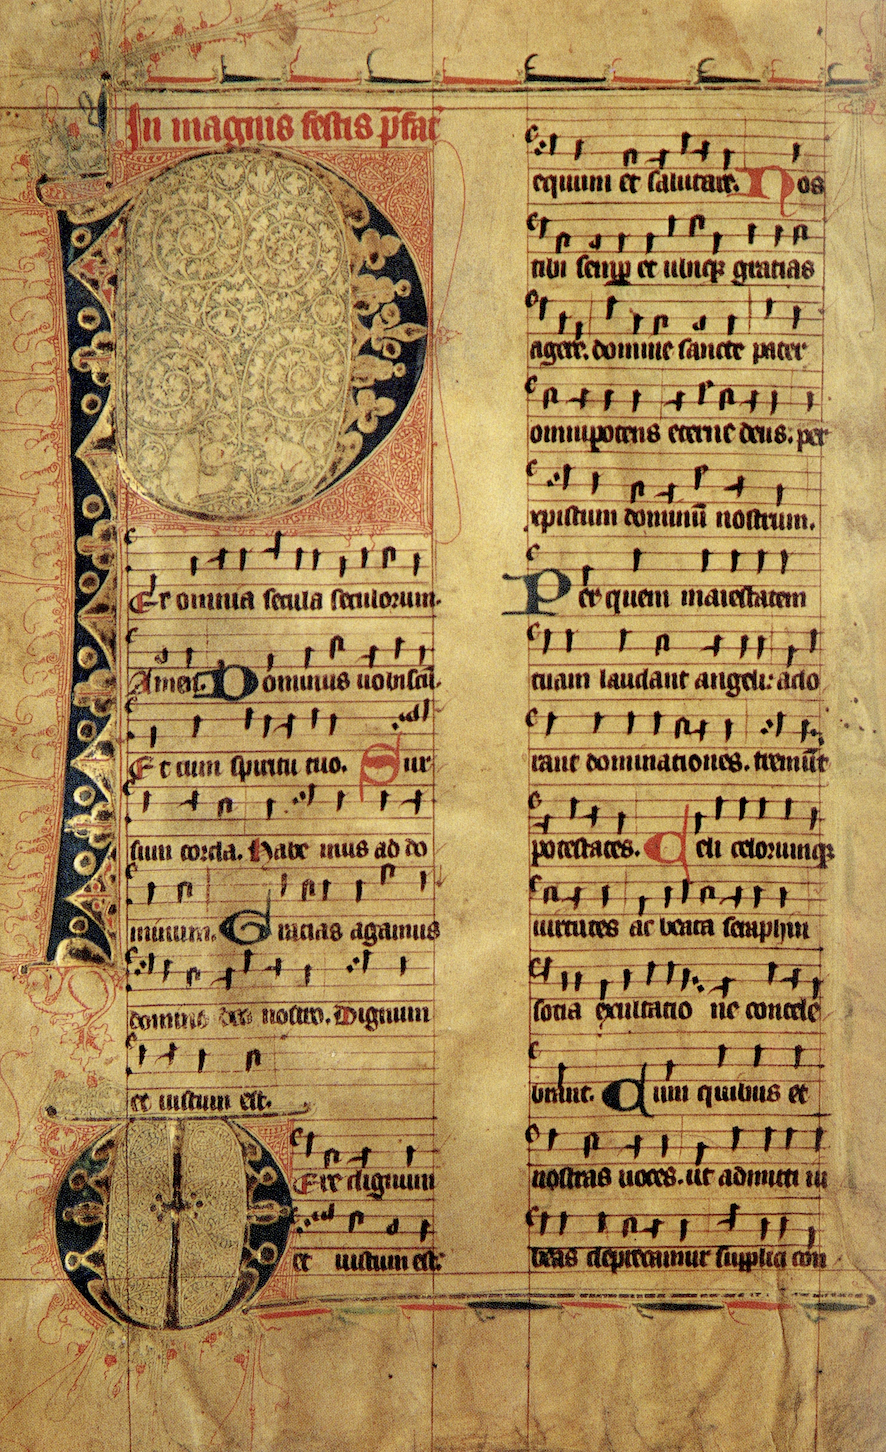
\includegraphics[width=7cm]{images/neume.png}
    \caption{ネウマ譜の例}
    \label{neume}
\end{figure}

\subsection{定量譜}
複数の奏者がそれぞれ異なった声部を同時に演奏する多声音楽が生まれると、リズム表示があいまいな従来のネウマ譜では不十分となった。
13世紀後半になると、音の長短を音符の形状で区別する定量譜(図\ref{teiryo})が利用されるようになった。

\begin{figure}[H]
    \centering
    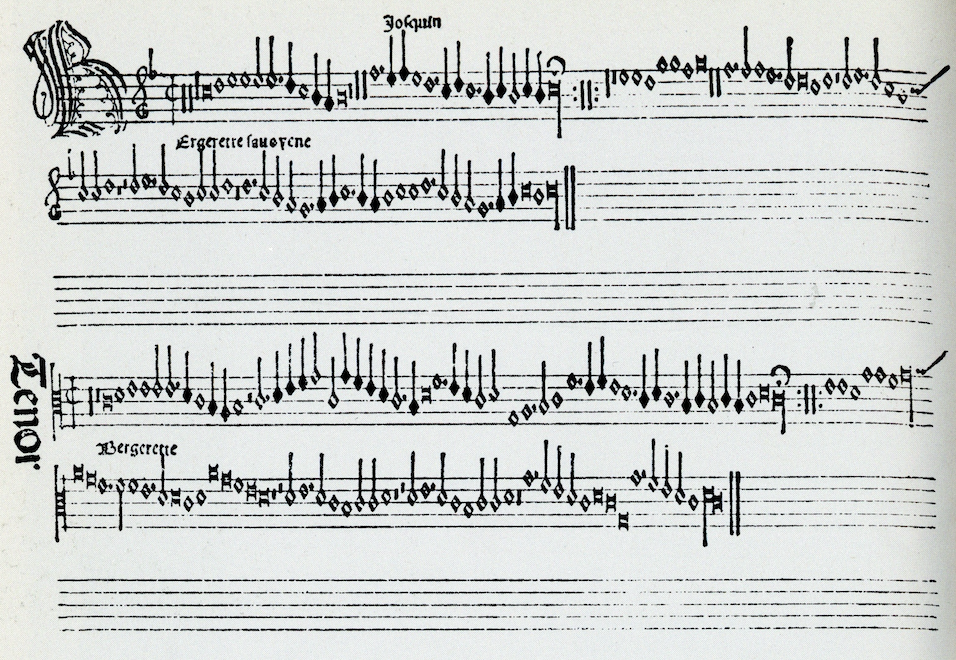
\includegraphics[width=9cm]{images/teiryo.png}
    \caption{定量譜の例}
    \label{teiryo}
\end{figure}

\subsection{奏法譜}
15世紀ごろからは特定の楽器の演奏法を具体的に表示する奏法譜(図\ref{tab})も広く利用された。
楽器ごとに固有の奏法譜をもち、現代でも「タブ譜」としてギター演奏に利用されている。

\begin{figure}[H]
    \centering
    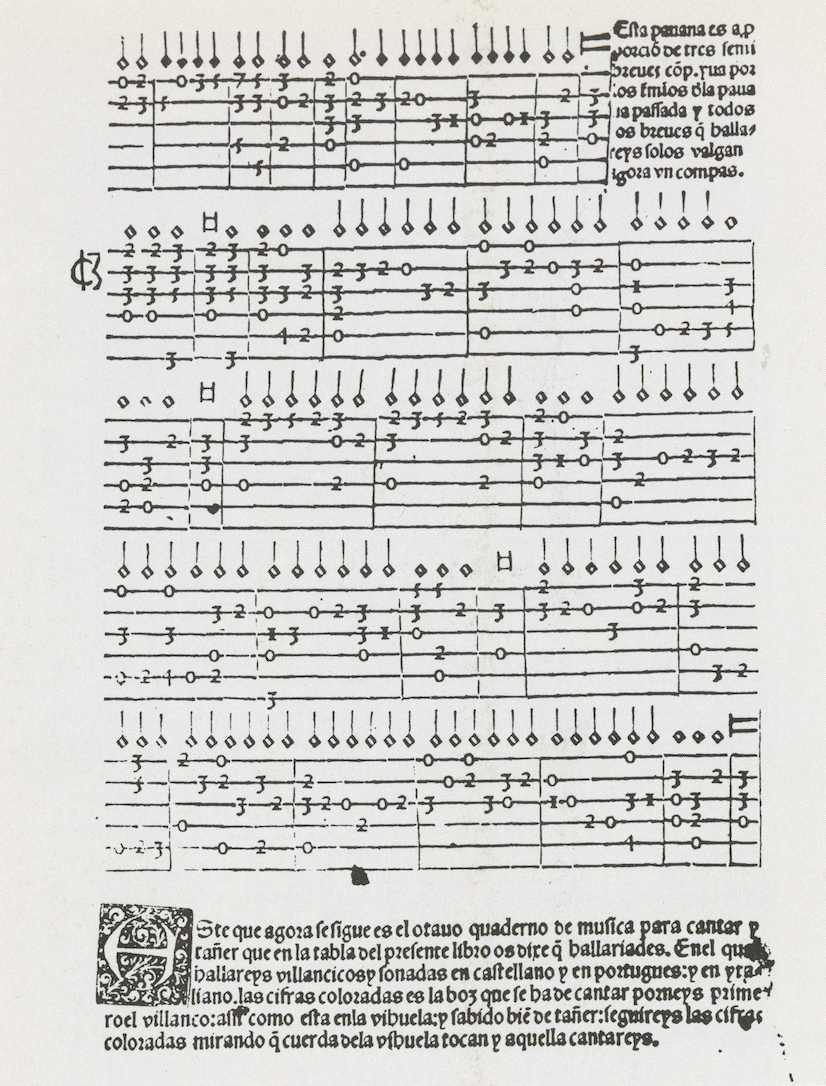
\includegraphics[width=6cm]{images/tab.png}
    \caption{奏法譜の例}
    \label{tab}
\end{figure}

\subsection{近代譜}
17世紀初頭から現在までに世界で最も普及している楽譜の形態(図\ref{kindai})で、鍵盤楽器用の奏法譜をルーツに持つ。
\begin{itemize}
    \item 五線による音高表示
    \item 音符の「はた」によるリズム表示
    \item 小節線の使用
\end{itemize}といった特徴がある。

\begin{figure}[H]
    \centering
    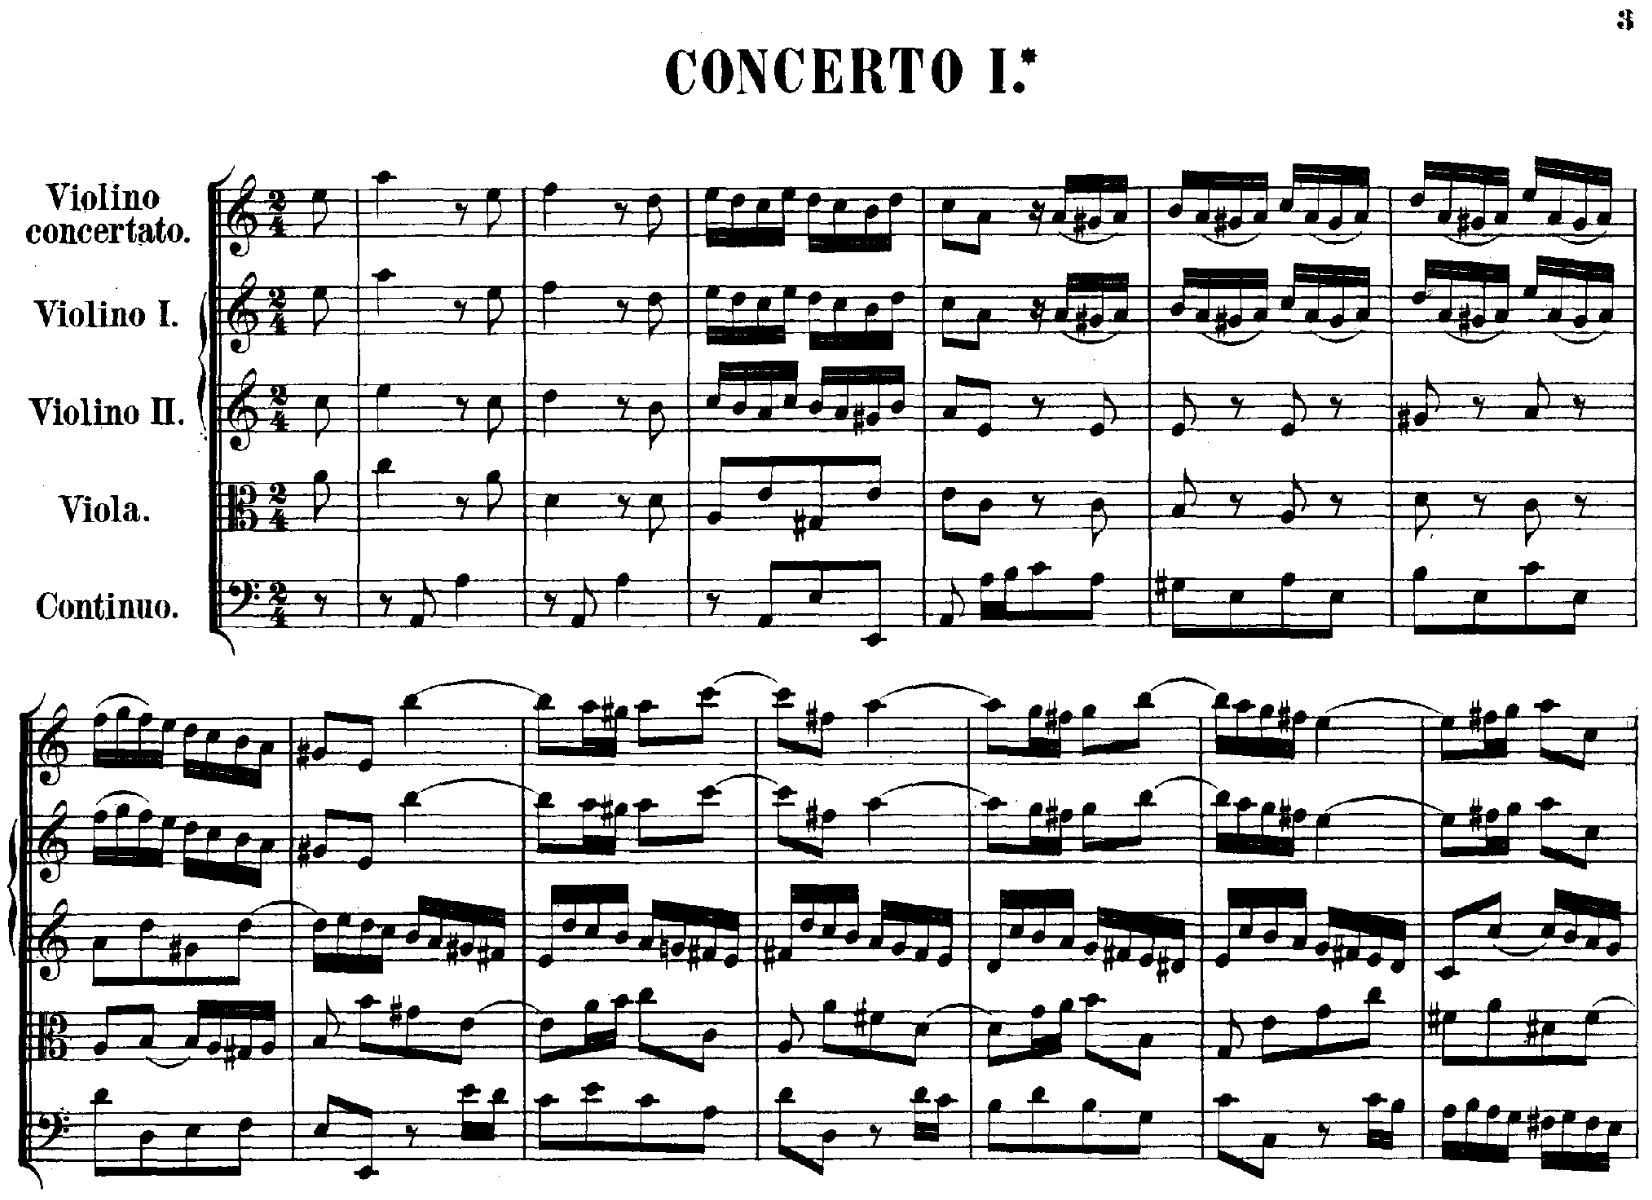
\includegraphics[width=9cm]{images/kindai.png}
    \caption{近代譜の例}
    \label{kindai}
\end{figure}

\subsection{現代音楽}
五線譜は鍵盤楽器をベースにした西洋音楽に最適化された記譜法のため、半音以下の繊細な音程のゆれや微妙なニュアンスを表現できないという制約がある。
現代の作曲家たちはそれぞれ独自の方法で克服しようと試みている(図\ref{kondo})。

\begin{figure}[H]
    \centering
    \includegraphics[width=9cm]{images/kondo.png}
    \caption{現代音楽譜の例}
    \label{kondo}
\end{figure}

\section{テキストの進化}
楽譜同様に紙の上で利用されていたテキストの進化にも注目する。
計算機が普及する以前のテキストは印刷物であるという制約から以下のような問題が存在した。
\begin{itemize}
    \item 簡単に編集できない
    \item せいぜい挿絵や写真程度の情報しか一緒に記録できない
    \item ドキュメントが複数存在するとき参照や管理が面倒
\end{itemize}

しかし現在では計算機の進化によりこれらの問題は完全に解決されている。
\begin{itemize}
    \item 手軽な編集\\
    計算機上でテキストを扱えるようになり、コピー/ペースト/Undo/Redoといったテキスト編集支援機能を搭載した各種エディタによって手軽な編集が可能になった。
    また印刷レイアウトを簡単に構成できるワープロソフトによって、美しいレイアウトの文章を簡単に作れるようになった。
    \item 手軽な入力\\
    日本語入力などの文字変換をサポートするシステム(IME)などによって手軽な入力が可能になった。
    \item マルチメディアの活用\\
    画像/音声/動画といったマルチメディアを自在に埋め込むことができるハイパーテキスト(図\ref{hy})によって、情報量の多いドキュメントの作成が可能になった。
    \item ハイパーリンク\\
    ハイパーテキストでは文章間リンクを示すハイパーリンク機能が利用でき、関連情報への素早いアクセスが可能になった。
    \item Web\\
    インターネット技術の進化とWebの普及によって、世界中に存在する様々なドキュメントへ瞬時にアクセスすることが可能になった。
    \item 共同編集\\
    Wikiのようなコラボレーションツールによって、場所や人数に制約を受けない共同編集が可能になった。
\end{itemize}


\begin{figure}[H]
    \centering
    \fbox{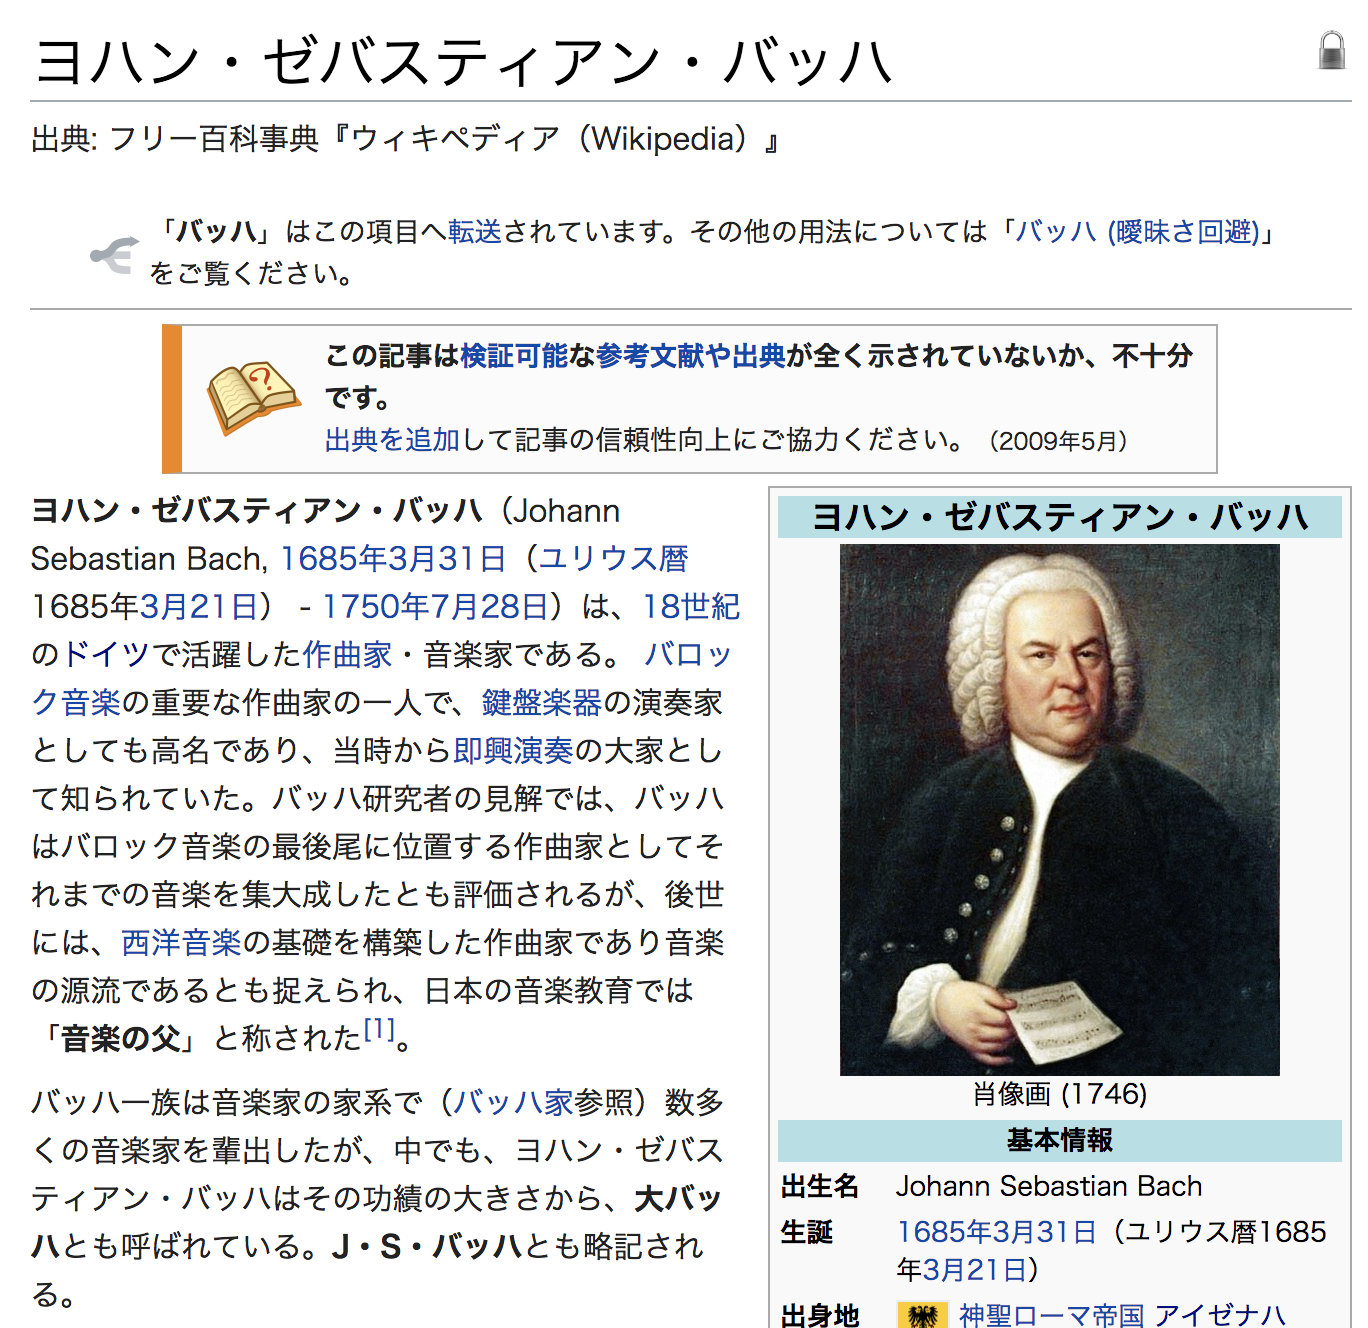
\includegraphics[width=9cm]{images/wikipedia.png}}
    \caption{ハイパーテキストの例}
    \label{hy}
\end{figure}

\section{楽譜の問題点}
\label{mondai}
一方、楽譜の性質は計算機の普及後も印刷物の時代から進化しておらず、以下のような問題が存在する。
\begin{enumerate}
    \item 簡単に編集できない\\
    現在流通している楽譜は紙やPDF形式での配布が一般的であり、内容の変更は前提とされていない。
    また自分で楽譜を書く場合は楽譜作成ソフトを利用できるが、印刷を前提としたレイアウトでの編集を強制されるため、一部だけアレンジしたい・1フレーズだけメモしたいといった用途には向いていない。
    \item メモなどの情報を自在に書けない\\
    楽譜を利用する際には、
    \begin{itemize}
        \item 演奏時に気付いたこと
        \item 演奏時に気をつけるべきこと
        \item 先生に習ったこと
    \end{itemize}などのメモを書き込みながら使うのが一般的である(図\ref{memo})。
    メモ書きできるのは余白スペースだけであり、楽譜自体に編集を加えてレイアウトを変更したり、音声や動画といった文字以外の情報を埋め込むことも不可能なので、記述できる内容は必然的に限られる。
    \item 参照や管理が面倒\\
    紙やPDFはそれぞれが独立しているため、手元の楽譜が増えると管理に苦労する。
    ファイル名でしか楽譜の内容を判断できないため、作曲者別にフォルダを分割するといったファイルの階層的な整理が必要である。
    また楽器構成や年代といった別の側面から参照したい場合には別途索引を用意しなければならない。
\end{enumerate}

\begin{figure}[H]
    \centering
    \fbox{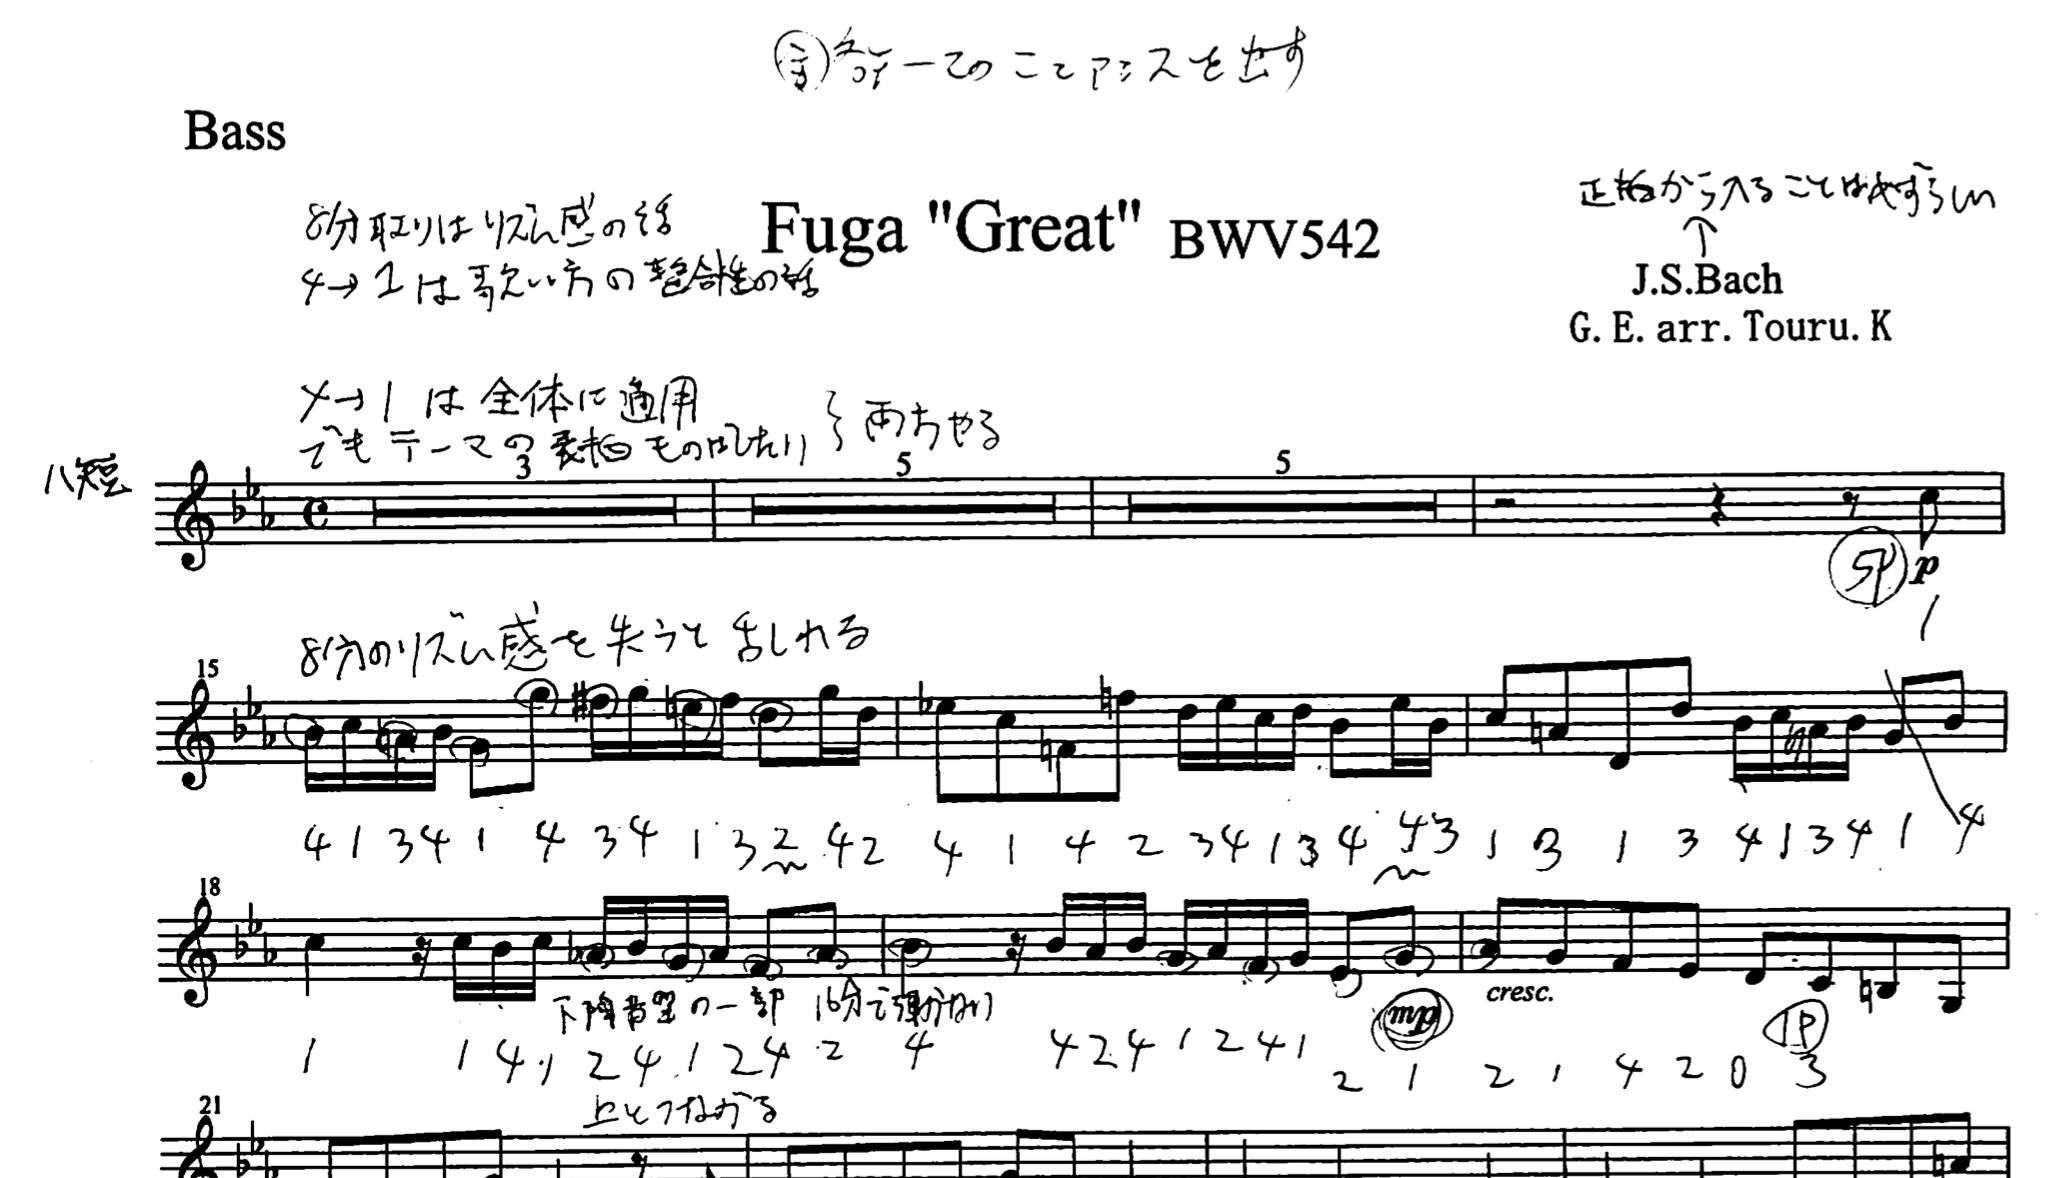
\includegraphics[width=10cm]{images/fuga.png}}
    \caption{楽譜上のメモの例}
    \label{memo}
\end{figure}

\section{既存の楽譜システム}
現在広く利用されている楽譜利用システムを解説する。
\subsection{楽譜作成ソフト}
Finale\footnote{\textsf{https://www.finalemusic.jp/}}(図\ref{finale})、Sibelius\footnote{\textsf{http://www.sibelius.jp/}}といった楽譜作成ソフトがデファクトスタンダードとして商用・私用問わず広く利用されている。
スタンプ感覚で音符を入力できるWYSIWYGな編集環境を持ち、以下のような楽譜作成支援機能を利用できる。
\begin{itemize}
    \item 楽譜スキャン・OCR
    \item パート譜自動作成
    \item レイアウトの細かい微調整
\end{itemize}

\begin{figure}[H]
    \centering
    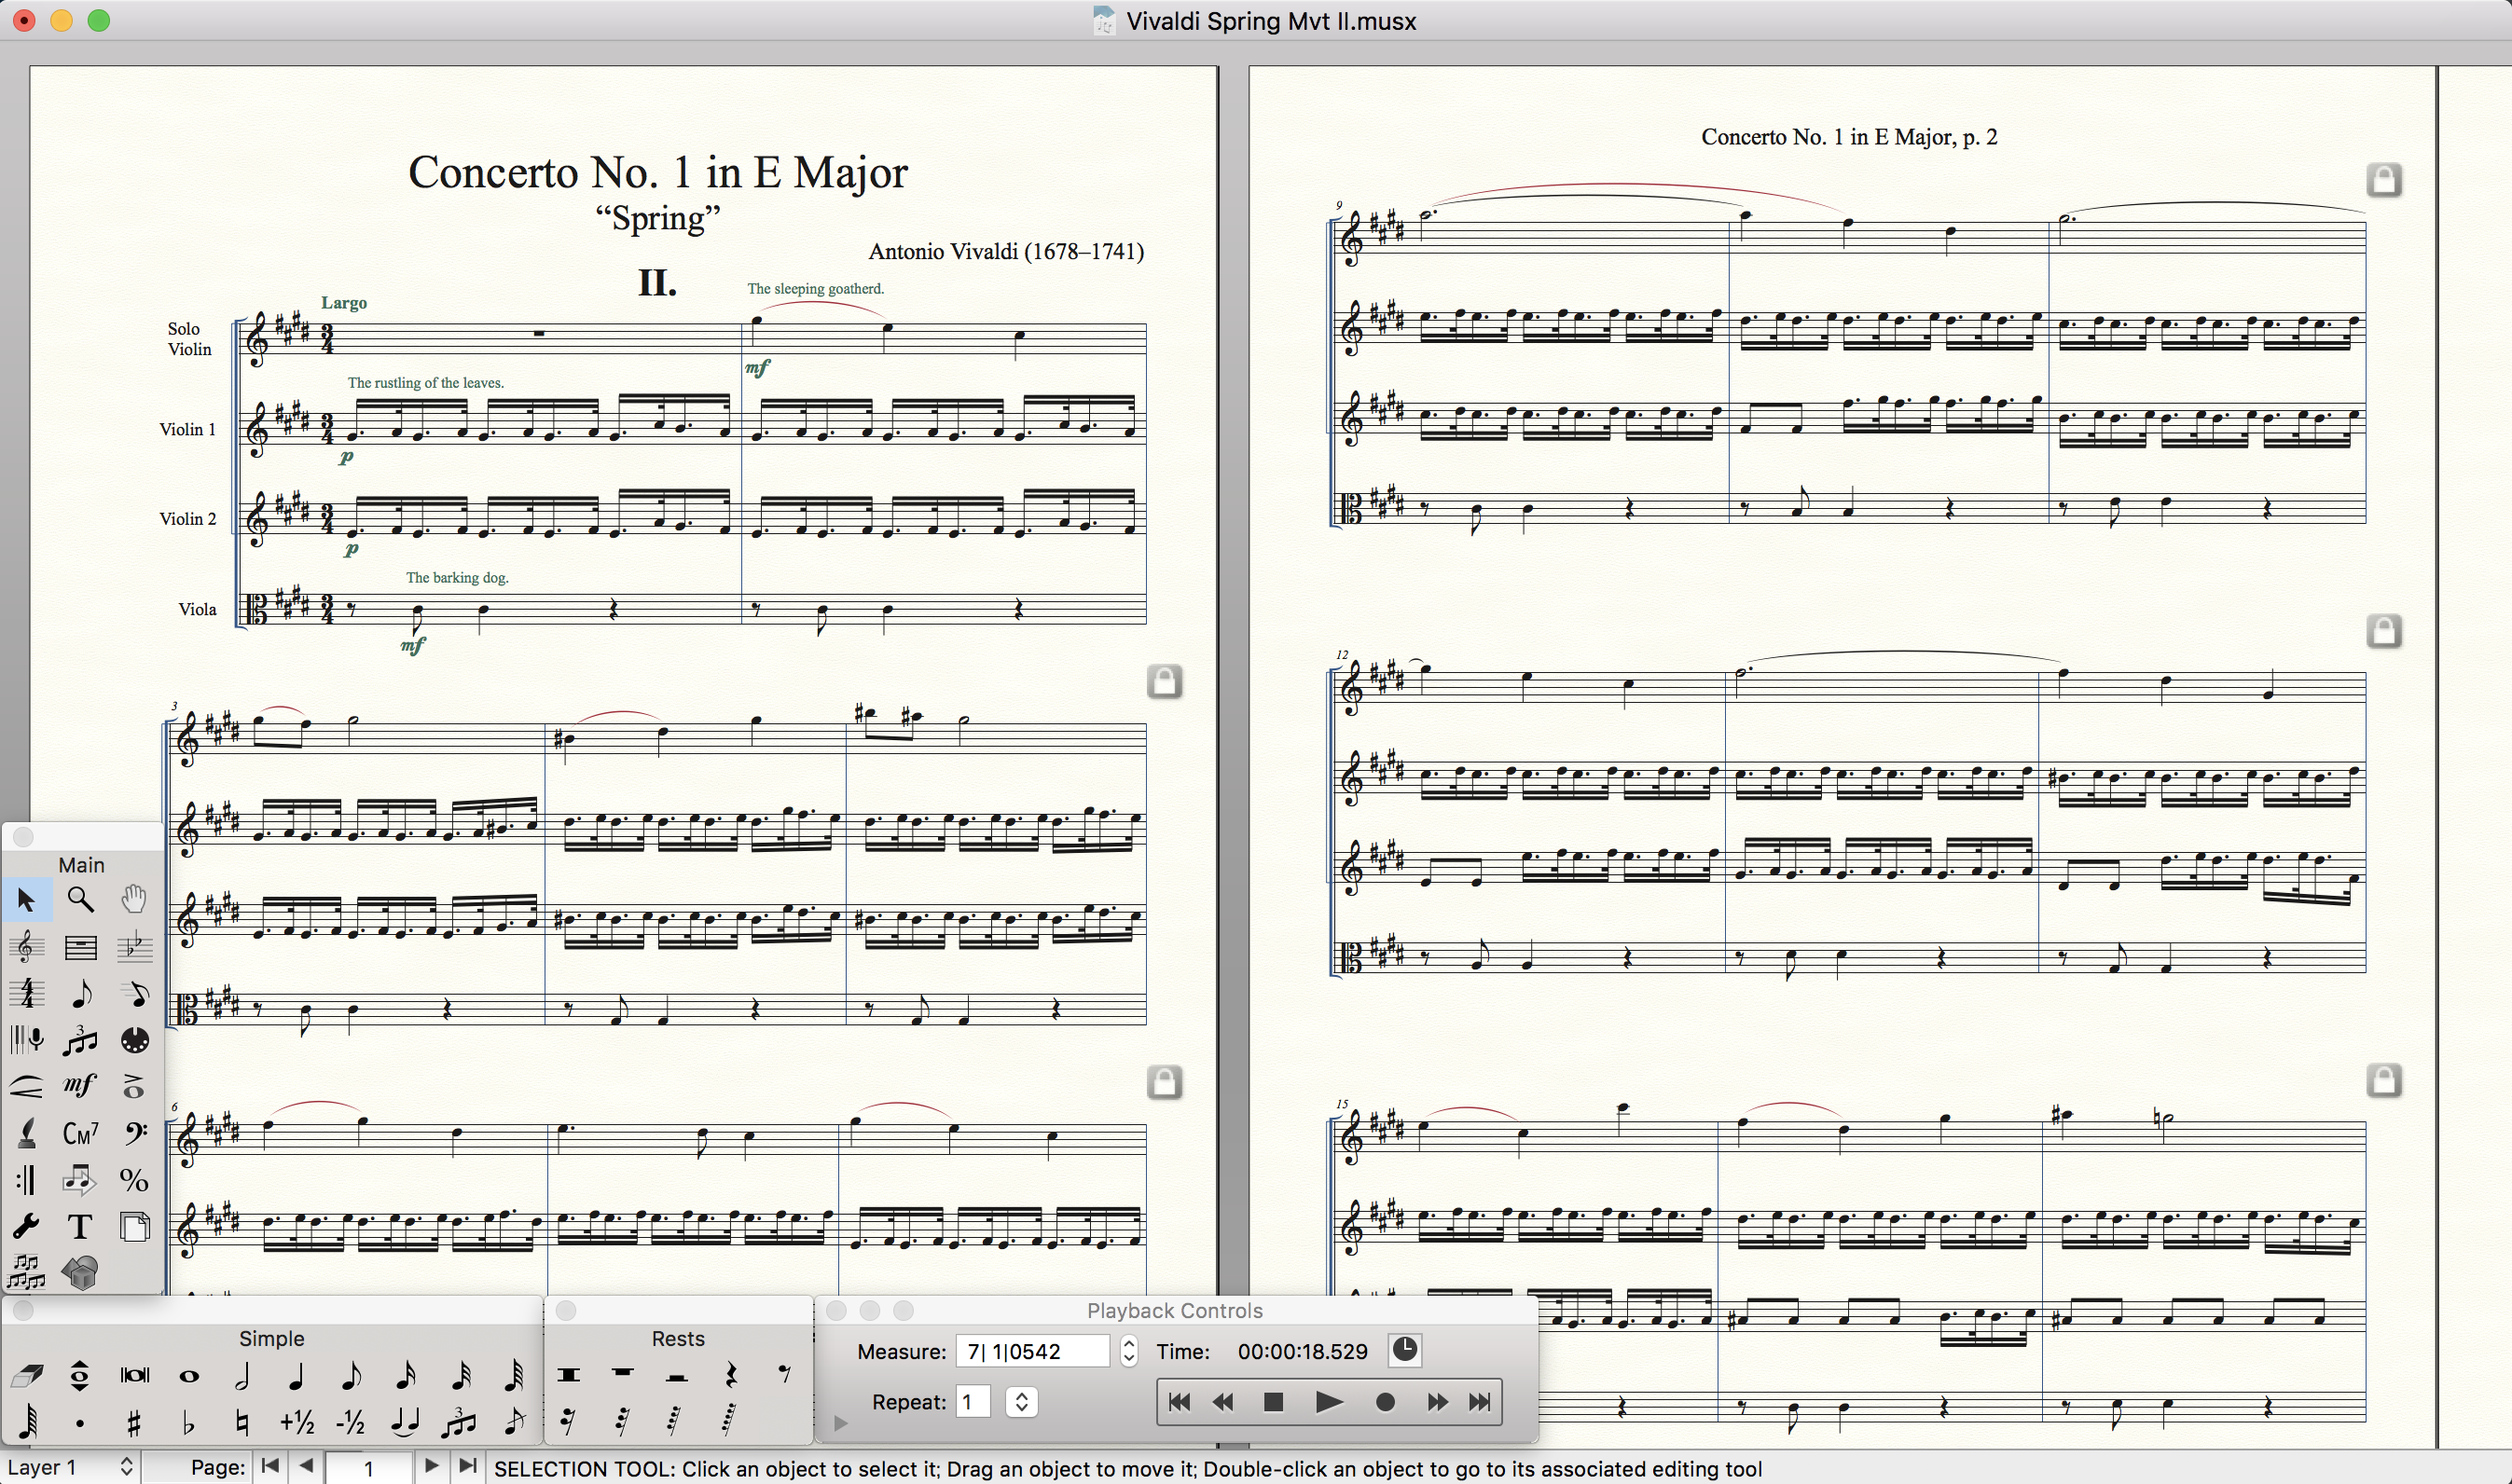
\includegraphics[width=10cm]{images/finale.png}
    \caption{Finaleの画面}
    \label{finale}
\end{figure}

\subsection{楽譜ビューアー}
ほとんどの楽譜はPDFファイルとして配布されるため、閲覧のために標準のPDFビューアーが利用されることが多い。
またPiascore\footnote{\textsf{http://piascore.com/}}(図\ref{pia})を代表とするタブレット端末向けの楽譜に特化したビューアーも広く普及しており、
\begin{itemize}
    \item 楽譜への書き込み
    \item 自動譜めくり
    \item メトロノーム
\end{itemize}といった機能を利用できる。

\begin{figure}[H]
    \centering
    \fbox{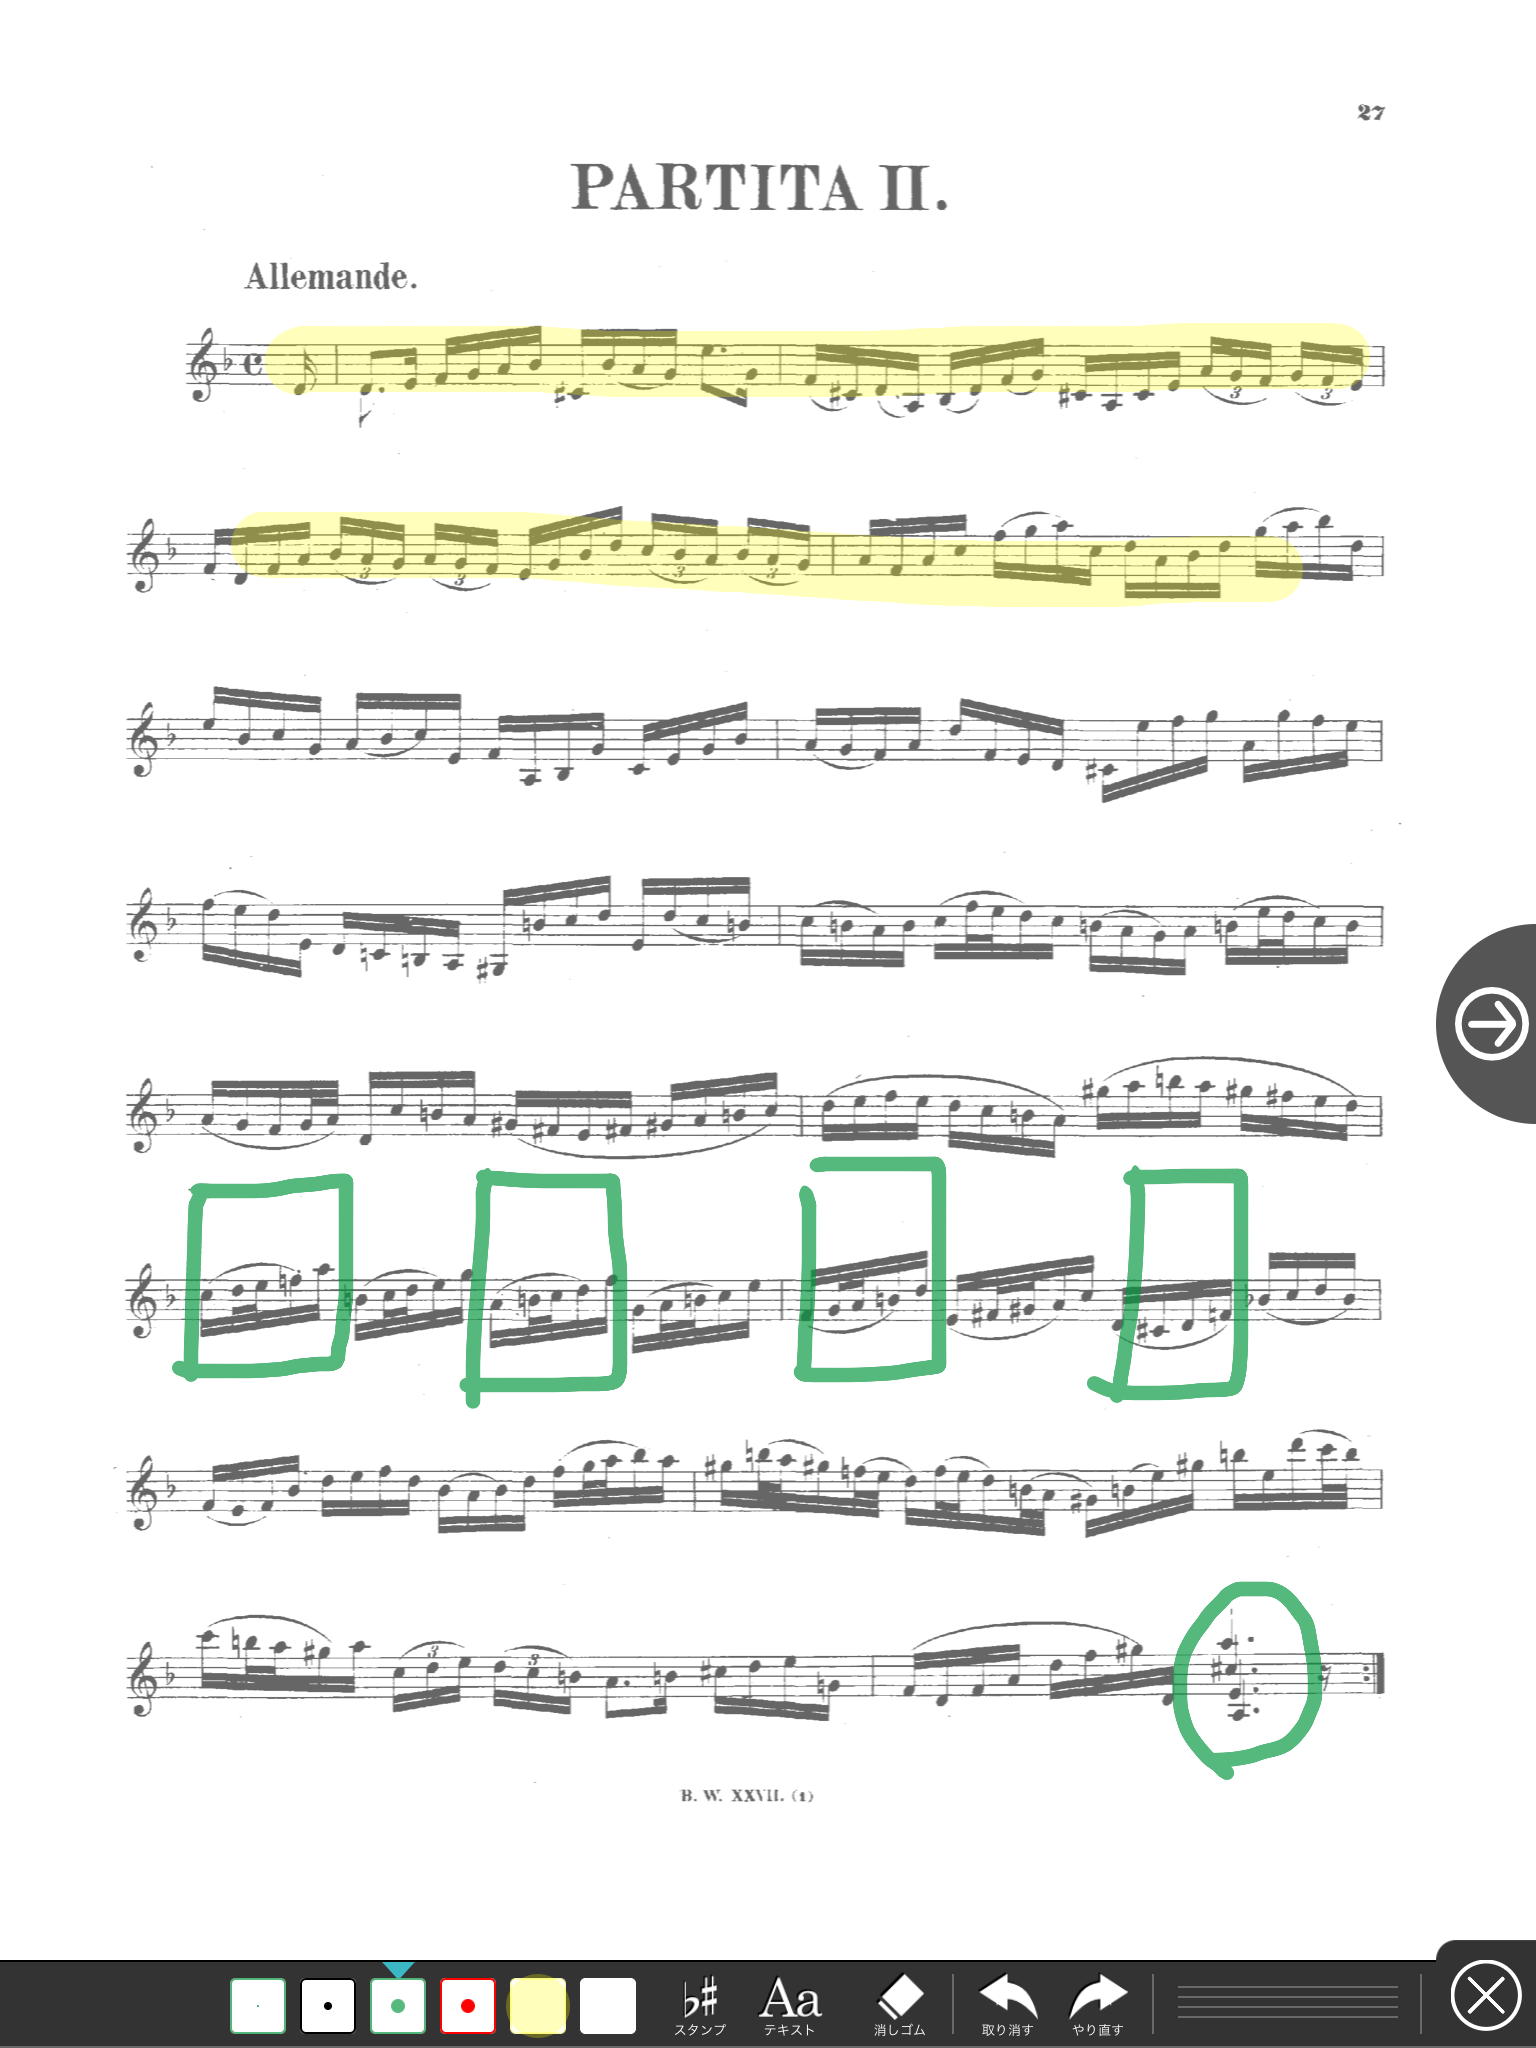
\includegraphics[width=8cm]{images/piascore.png}}
    \caption{Piascoreの画面}
    \label{pia}
\end{figure}

\section{まとめ}
楽譜の編集や閲覧を支援するシステムが広く利用されているが、これらは計算機上で楽譜の利用形態を再現したに過ぎず、
\begin{enumerate}
    \item 簡単に編集できない
    \item メモなどの情報を自在に書けない
    \item 参照や管理が面倒
\end{enumerate}という本質的な楽譜の問題は解決されていない。
次章では上記のような楽譜が持つ問題点を解決し、これまでの楽譜の在り方にとらわれない次世代の楽譜システム「ハイパー楽譜システム」を提案する。
  % 本文2
\chapter{設計}
\label{chap:sekkei}

本章ではハイパー楽譜システムの要件と設計について述べる。

\newpage

\section{要件}
前章で整理した楽譜の問題点を踏まえた上で、ハイパー楽譜システムの要件を整理する。
\begin{enumerate}
    \item 楽譜を簡単に編集できる\\
    メモを取るような気軽さで楽譜を書くことができ、新規作成/既存楽譜の編集両方を簡単に行える。
    \item メモなどの情報を自在に書ける\\
    テキストで楽譜を記述でき、ハイパーテキストのようなフォーマットの中で楽譜以外の情報も一緒に管理できる。
    \item ハイパーリンクを利用できる\\
    楽譜上の要素やテキストに対してハイパーリンクを設定でき、関連情報に素早くアクセスできる。
\end{enumerate}
この要件を満たす楽譜システムは、ハイパーテキストの編集環境であるWikiと、テキストベースの楽譜記述言語の組み合わせによって実現できる。

\section{ハイパー楽譜システム}
本研究で提案するハイパー楽譜システムの基本構成と使い方を解説する。

\subsection{基本構成}
ハイパー楽譜システム(図\ref{hs})はWikiであるScrapbox\footnote{\textsf{https://scrapbox.io}}と、楽譜記述言語のABC記譜法\footnote{\textsf{http://abcnotation.com}}(以下ABC)によって構成されている。

\begin{figure}[H]
    \centering
    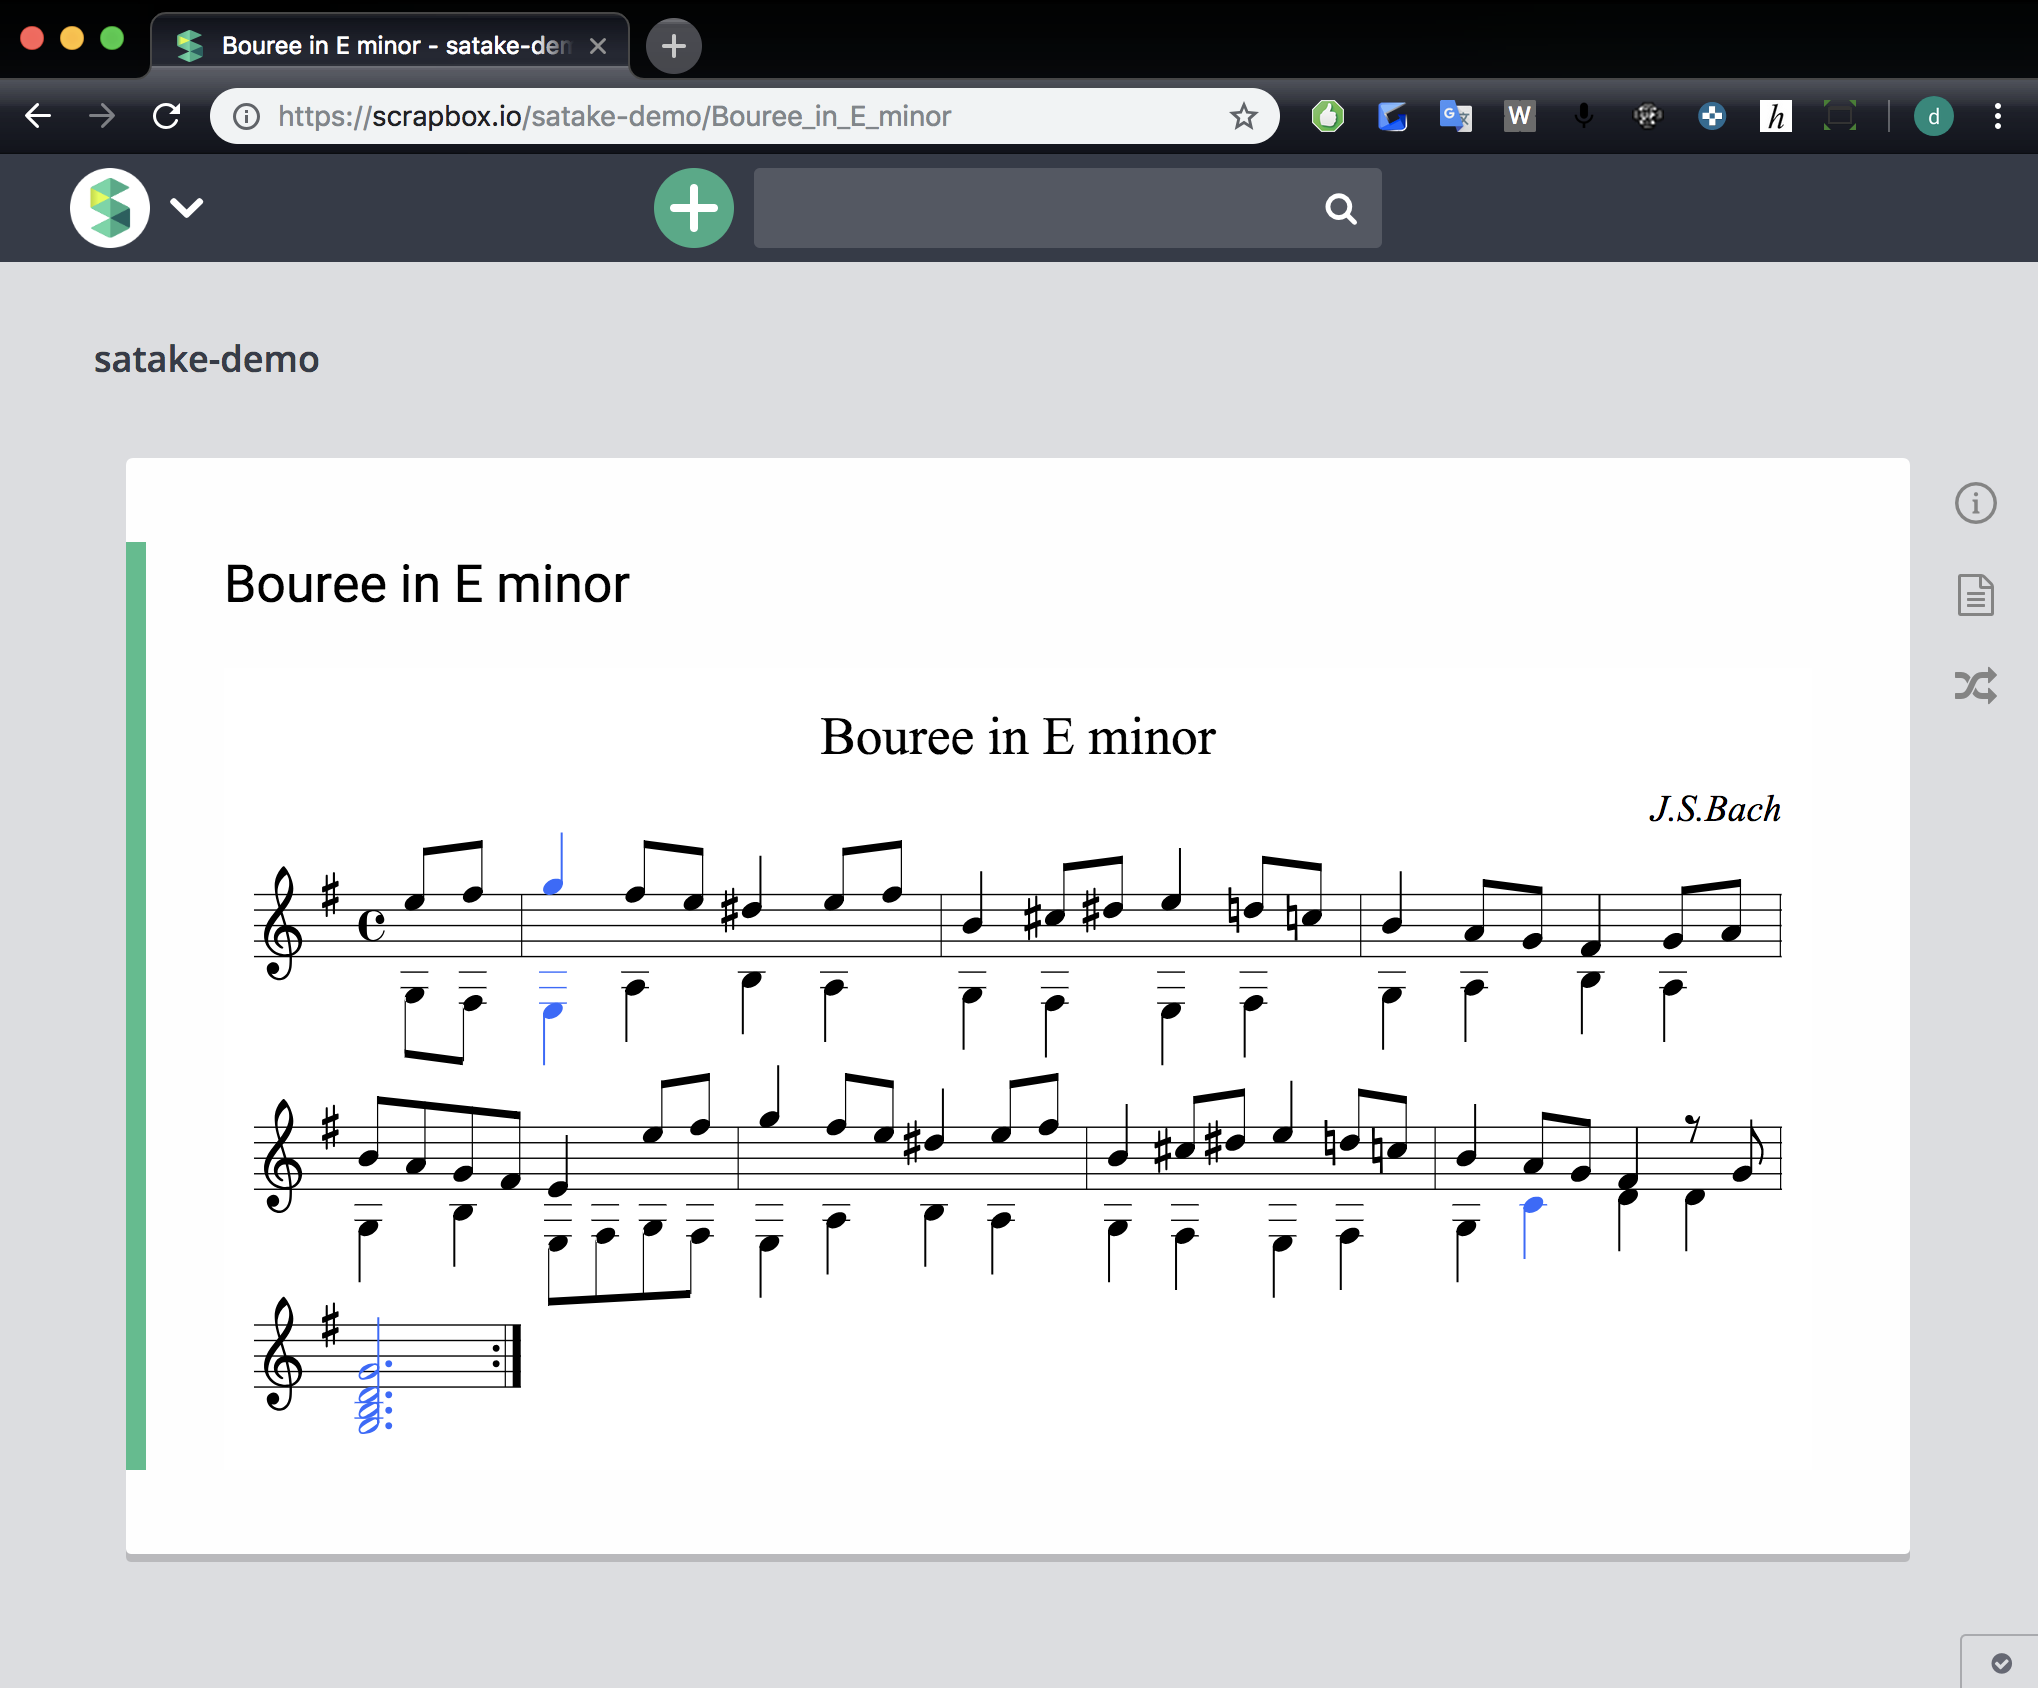
\includegraphics[width=10cm]{images/hyperscore.png}
    \caption{ハイパー楽譜システム上で書かれた楽譜}
    \label{hs}
\end{figure}


\paragraph*{Scrapbox}
Scrapbox(図\ref{scrap})はGyazz\cite{Gyazz}をベースにして開発された、Nota\footnote{\textsf{https://www.notainc.com/ja}}社が運営しているWikiである。
他のシステムには存在しない、ハイパー楽譜システムとして利用するのに最適な特徴を持つ。

\begin{itemize}
    \item シンプルで柔軟な記法をもつWYSIWYGエディタ

    入力/改行/段落/箇条書きといった基本的なテキスト編集を見たまま行える。
    またリンクやマルチメディアの埋め込みには\texttt{[]}記法のみで対応でき、他に様々な記法を覚える必要がない。

    \begin{itembox}[l]{\texttt{[]}記法}
        \begin{tabbing}
            ********************************* \= ********************** \kill
            \texttt{[ページ名]} \> 同一Wiki内ページへのリンク\\
            \texttt{[URL]} \> 外部リンク\\
            \texttt{[画像URL]} \> 画像埋め込み\\
            \texttt{[音声URL]} \> 音声埋め込み\\
            \texttt{[YouTube/VimeoURL]} \> 動画埋め込み\\
            \texttt{[GoogleMapsURL]} \> 地図埋め込み
        \end{tabbing}
    \end{itembox}

    \item 関連ページリスト

    Scrapboxページの下部には
    \begin{itemize}
        \item 別ページへのリンク
        \item 別ページからのリンク
        \item リンク先ページがリンクしているページ
    \end{itemize}といった関連ページリスト(図\ref{related})が表示され、どのような情報と関連するのか一目瞭然に分かる。

    \item リアルタイム共同編集

    Scrapboxでは複数人による共同編集だけでなく、Googleドキュメント\footnote{\textsf{https://www.google.com/intl/ja\_jp/docs/about}}のようなリアルタイム編集作業をコンフリクトすることなく行うことが可能である。
\end{itemize}

\begin{figure}[H]
    \centering
    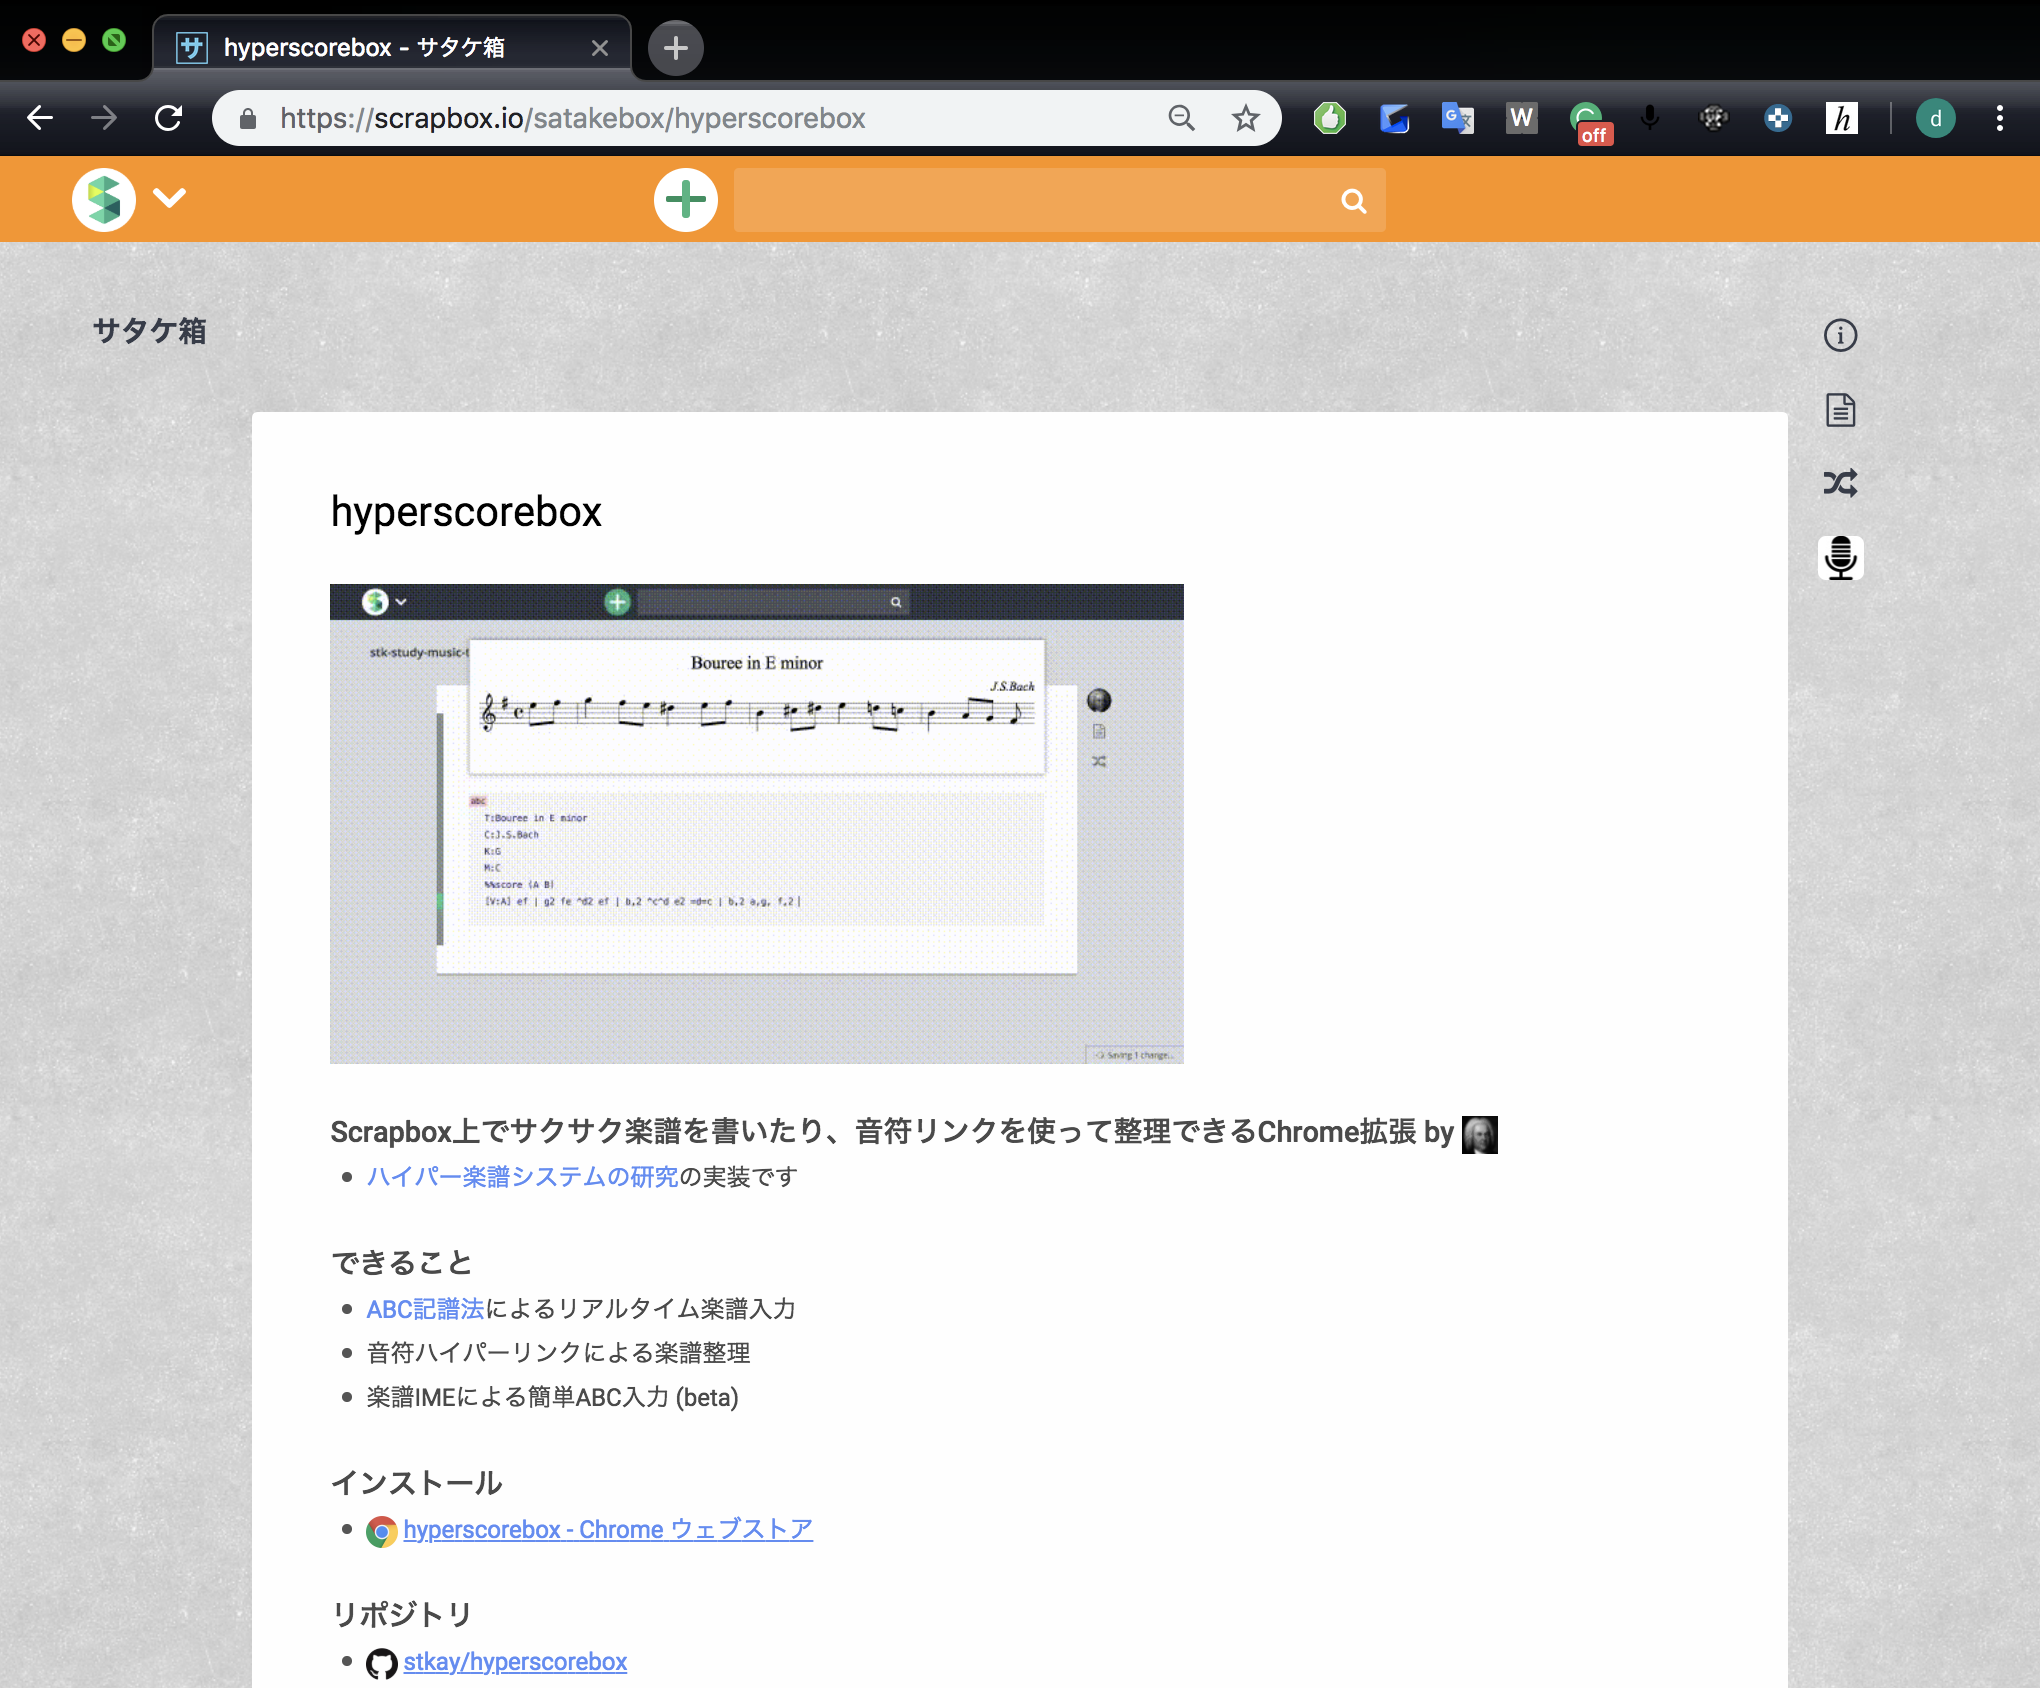
\includegraphics[width=10cm]{images/scrapbox.png}
    \caption{Scrapboxの画面}
    \label{scrap}
\end{figure}

\begin{figure}[H]
    \centering
    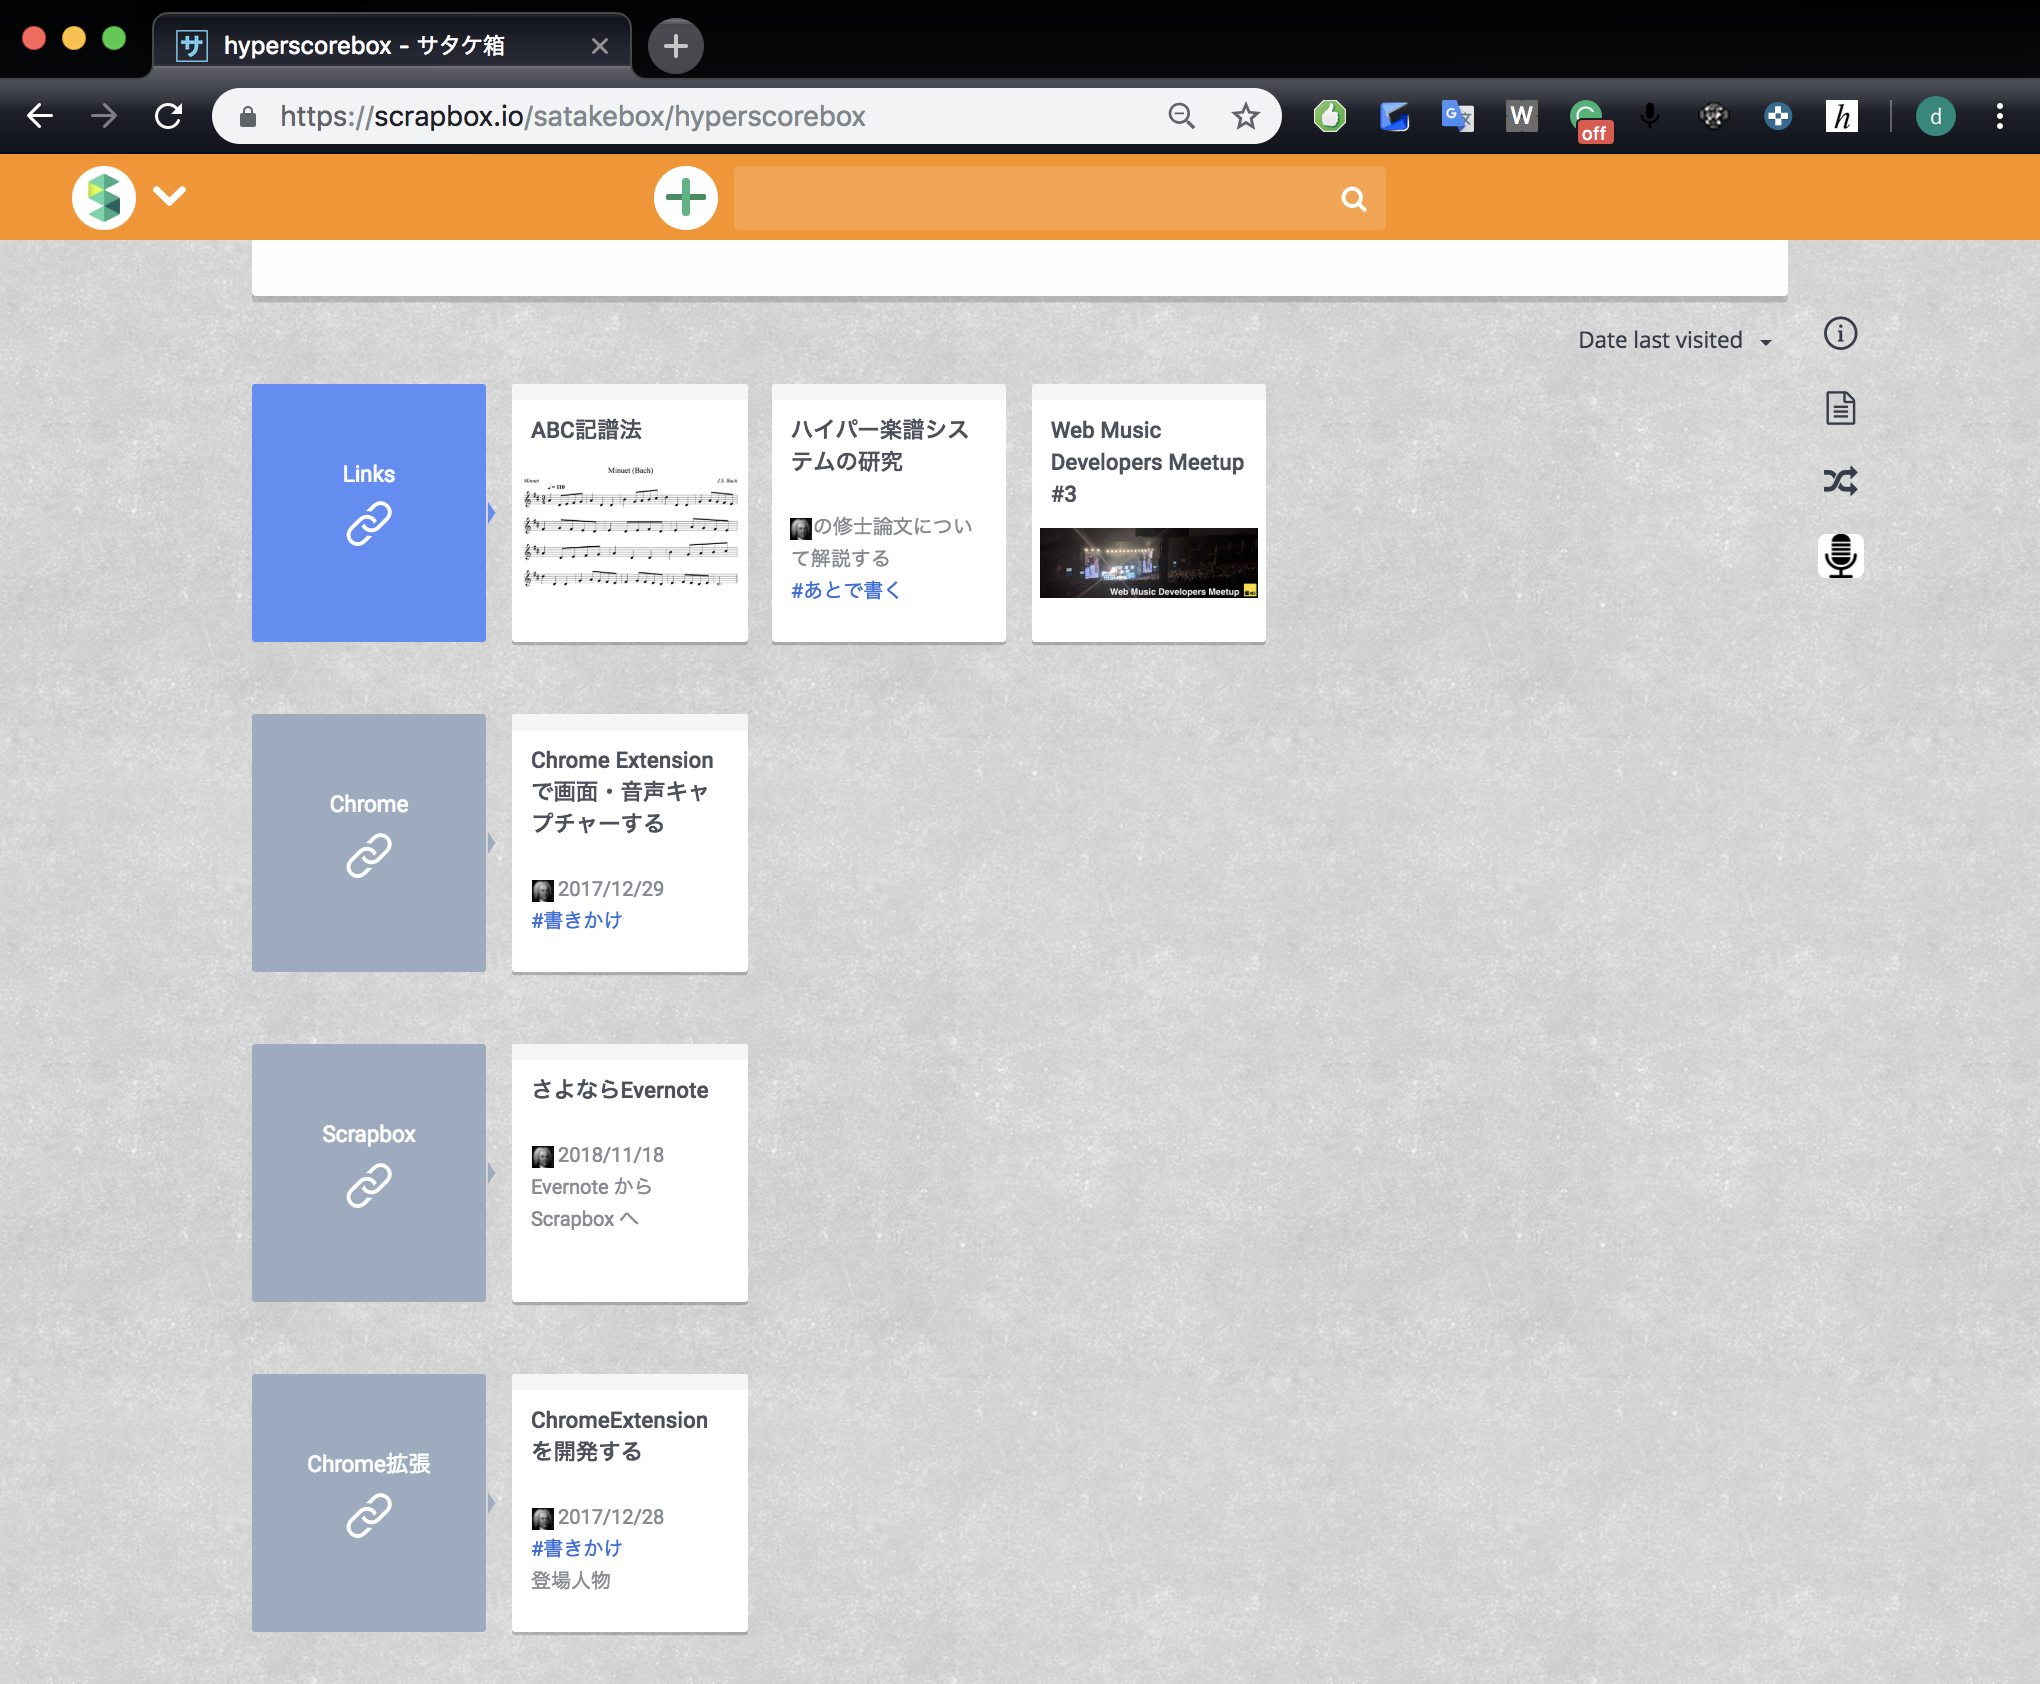
\includegraphics[width=10cm]{images/related.png}
    \caption{関連ページリスト}
    \label{related}
\end{figure}

\paragraph*{ABC}
ABCはプレーンテキスト形式の楽譜記述言語で、\texttt{c}が「ド」を表すシンプルな記法(ソースコード\ref{abctext})を持つ。
大規模で複雑な楽譜(図\ref{complex})の記述も可能で、幅広いシーンで利用可能である。
利用者コミュニティ\footnote{\textsf{https://groups.yahoo.com/neo/groups/abcusers/info}}が活発でバージョンのアップデートが頻繁に行われていたり、ユーザーによる譜例が多く公開されていることから信頼できるフォーマットである。
ブラウザからはJavaScriptライブラリのabcjs\footnote{\textsf{https://abcjs.net/}}が利用でき、既存の楽譜システムと比較しても遜色のない綺麗な楽譜を出力することが可能である。

\begin{lstlisting}[caption=「ド」を表すABC, label=abctext]
    c
\end{lstlisting}
\begin{figure}[H]
\centering
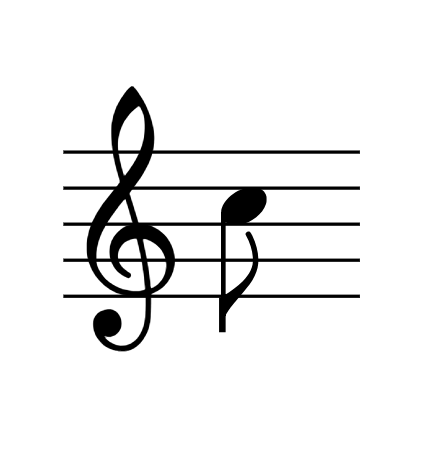
\includegraphics[width=2cm]{images/c.png}
\caption{「ド」の譜例}
\label{abcnote}
\end{figure}

\begin{figure}[H]
\centering
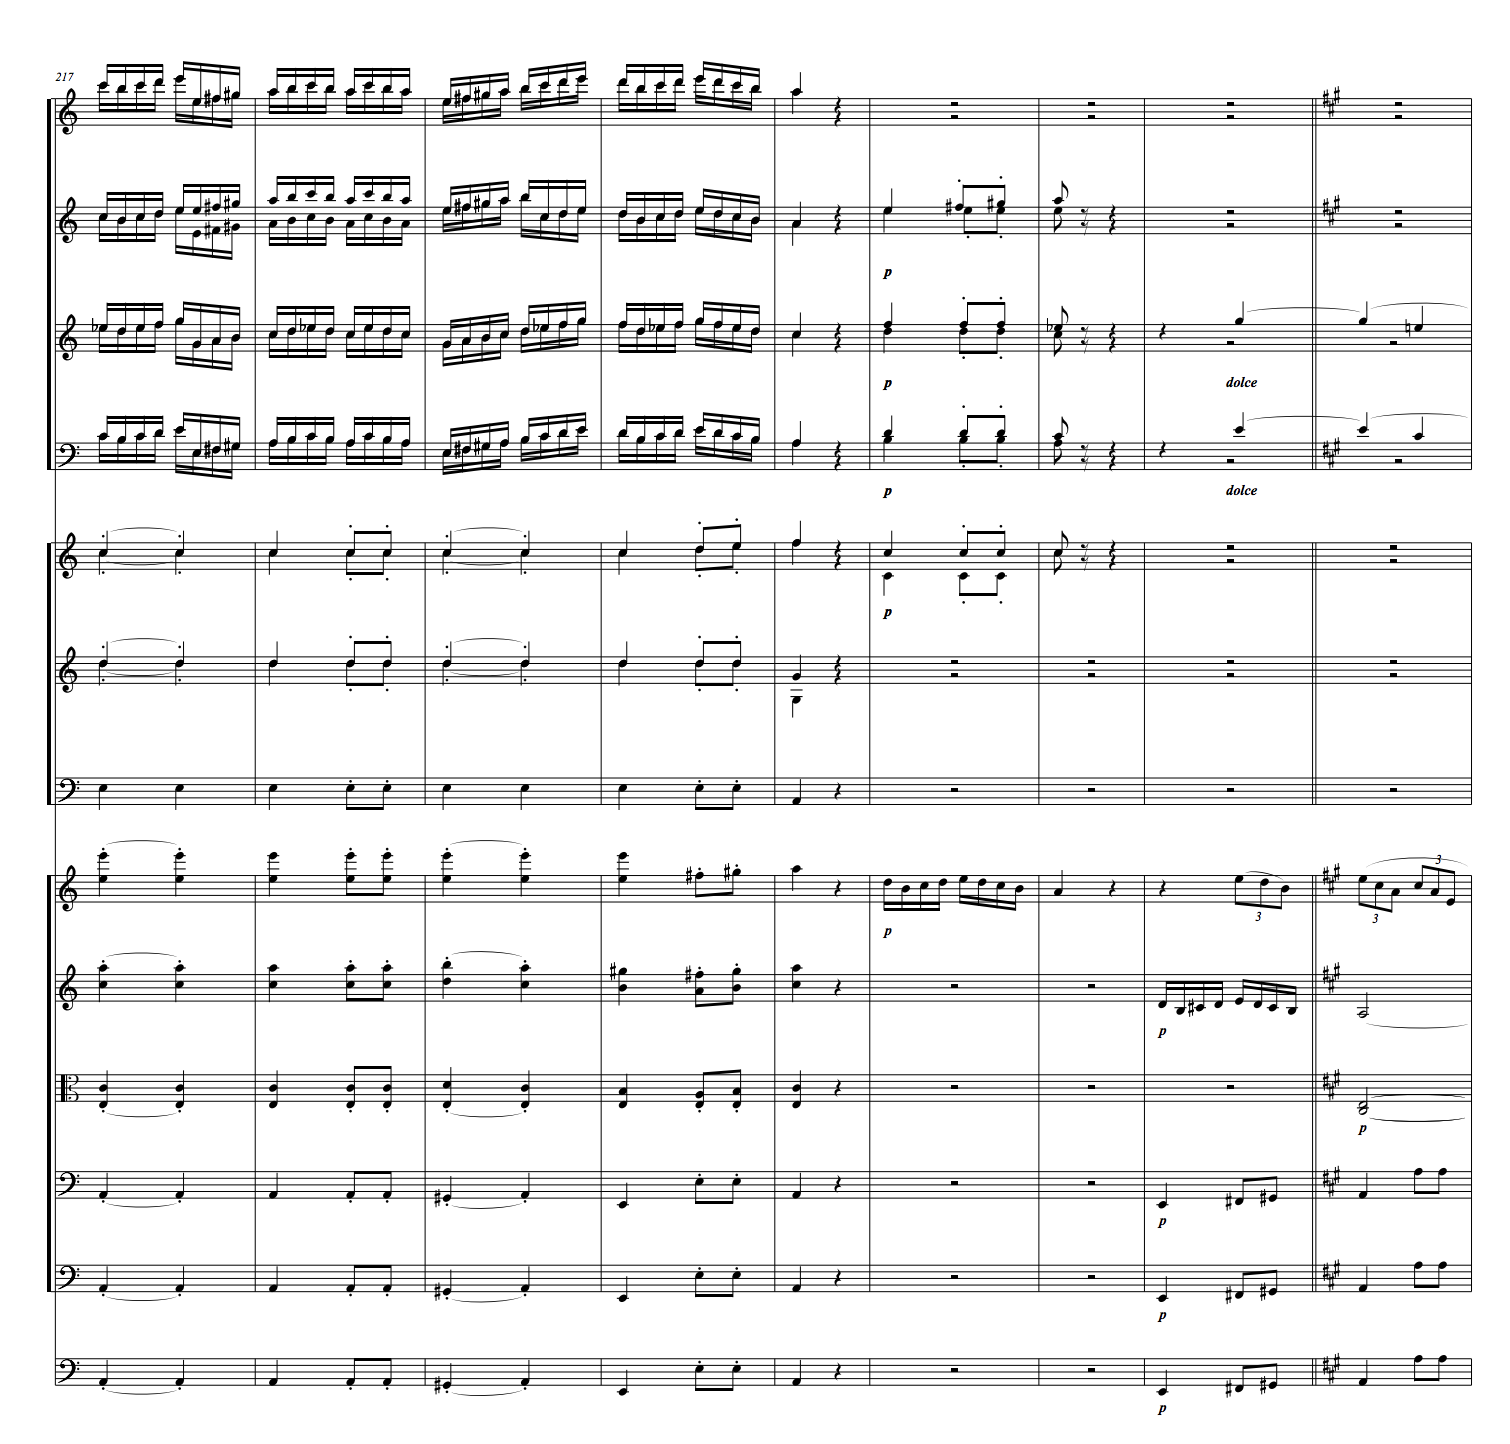
\includegraphics[width=10cm]{images/complexabc.png}
\caption{複雑な楽譜の例}
\label{complex}
\end{figure}


\subsection{使い方}
\paragraph*{楽譜を書く}
Scrapbox上で\texttt{code:*.abc}という行に続けてABCテキストを書くとABC記述の真上に楽譜画像が表示され(図\ref{editingabc})、楽譜を確認しながらリアルタイムに編集できる。
楽譜やABCの領域外をクリックするとABC記述が隠れ、楽譜のみが表示される(図\ref{editedabc})。

\begin{figure}[H]
\centering
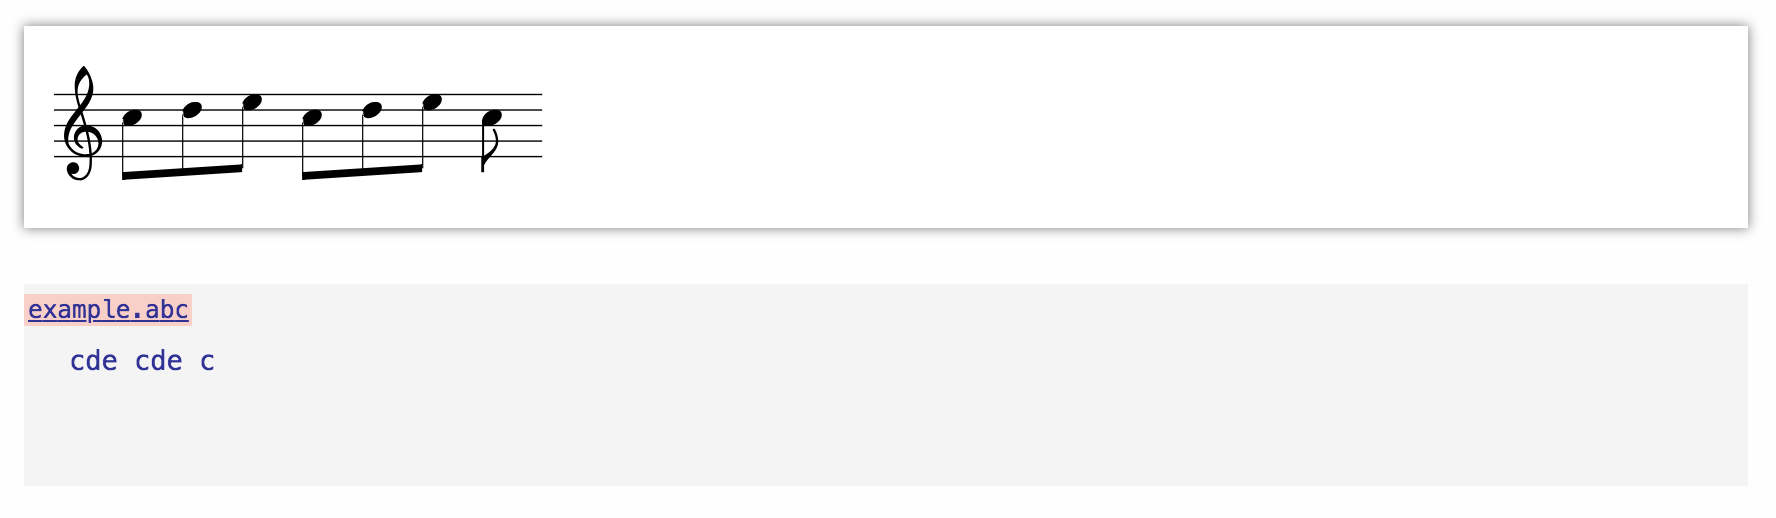
\includegraphics[width=10cm]{images/editingabc.png}
\caption{編集中の楽譜}
\label{editingabc}
\end{figure}

\begin{figure}[H]
\centering
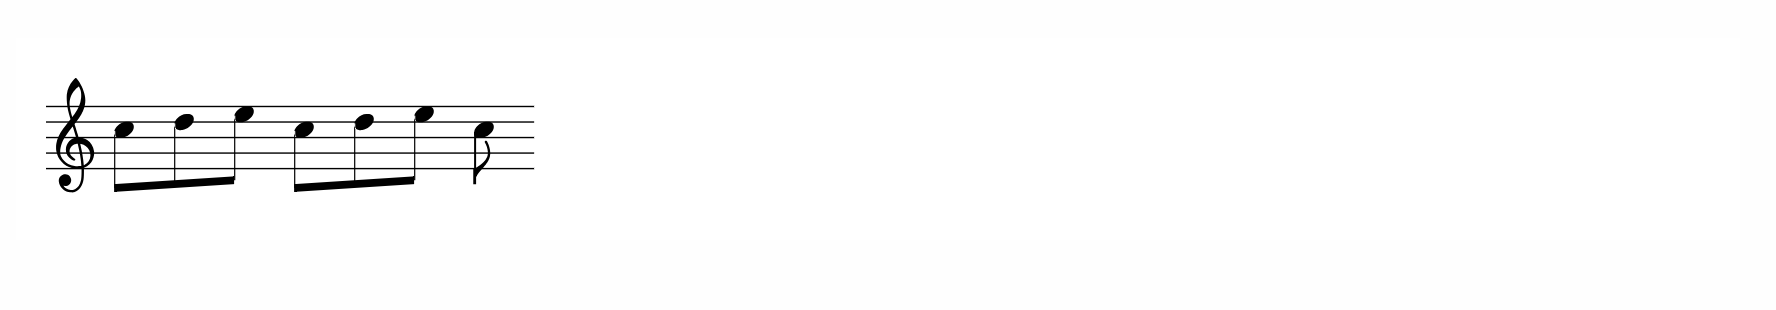
\includegraphics[width=10cm]{images/editedabc.png}
\caption{編集後の楽譜}
\label{editedabc}
\end{figure}


\paragraph*{音符など以外の情報を書く}
楽譜領域以外では標準のScrapbox記法を利用できるので、自在にテキストを書いたり、マルチメディアを埋め込むことができる(図\ref{scoreandtext})。

\begin{figure}[H]
\centering
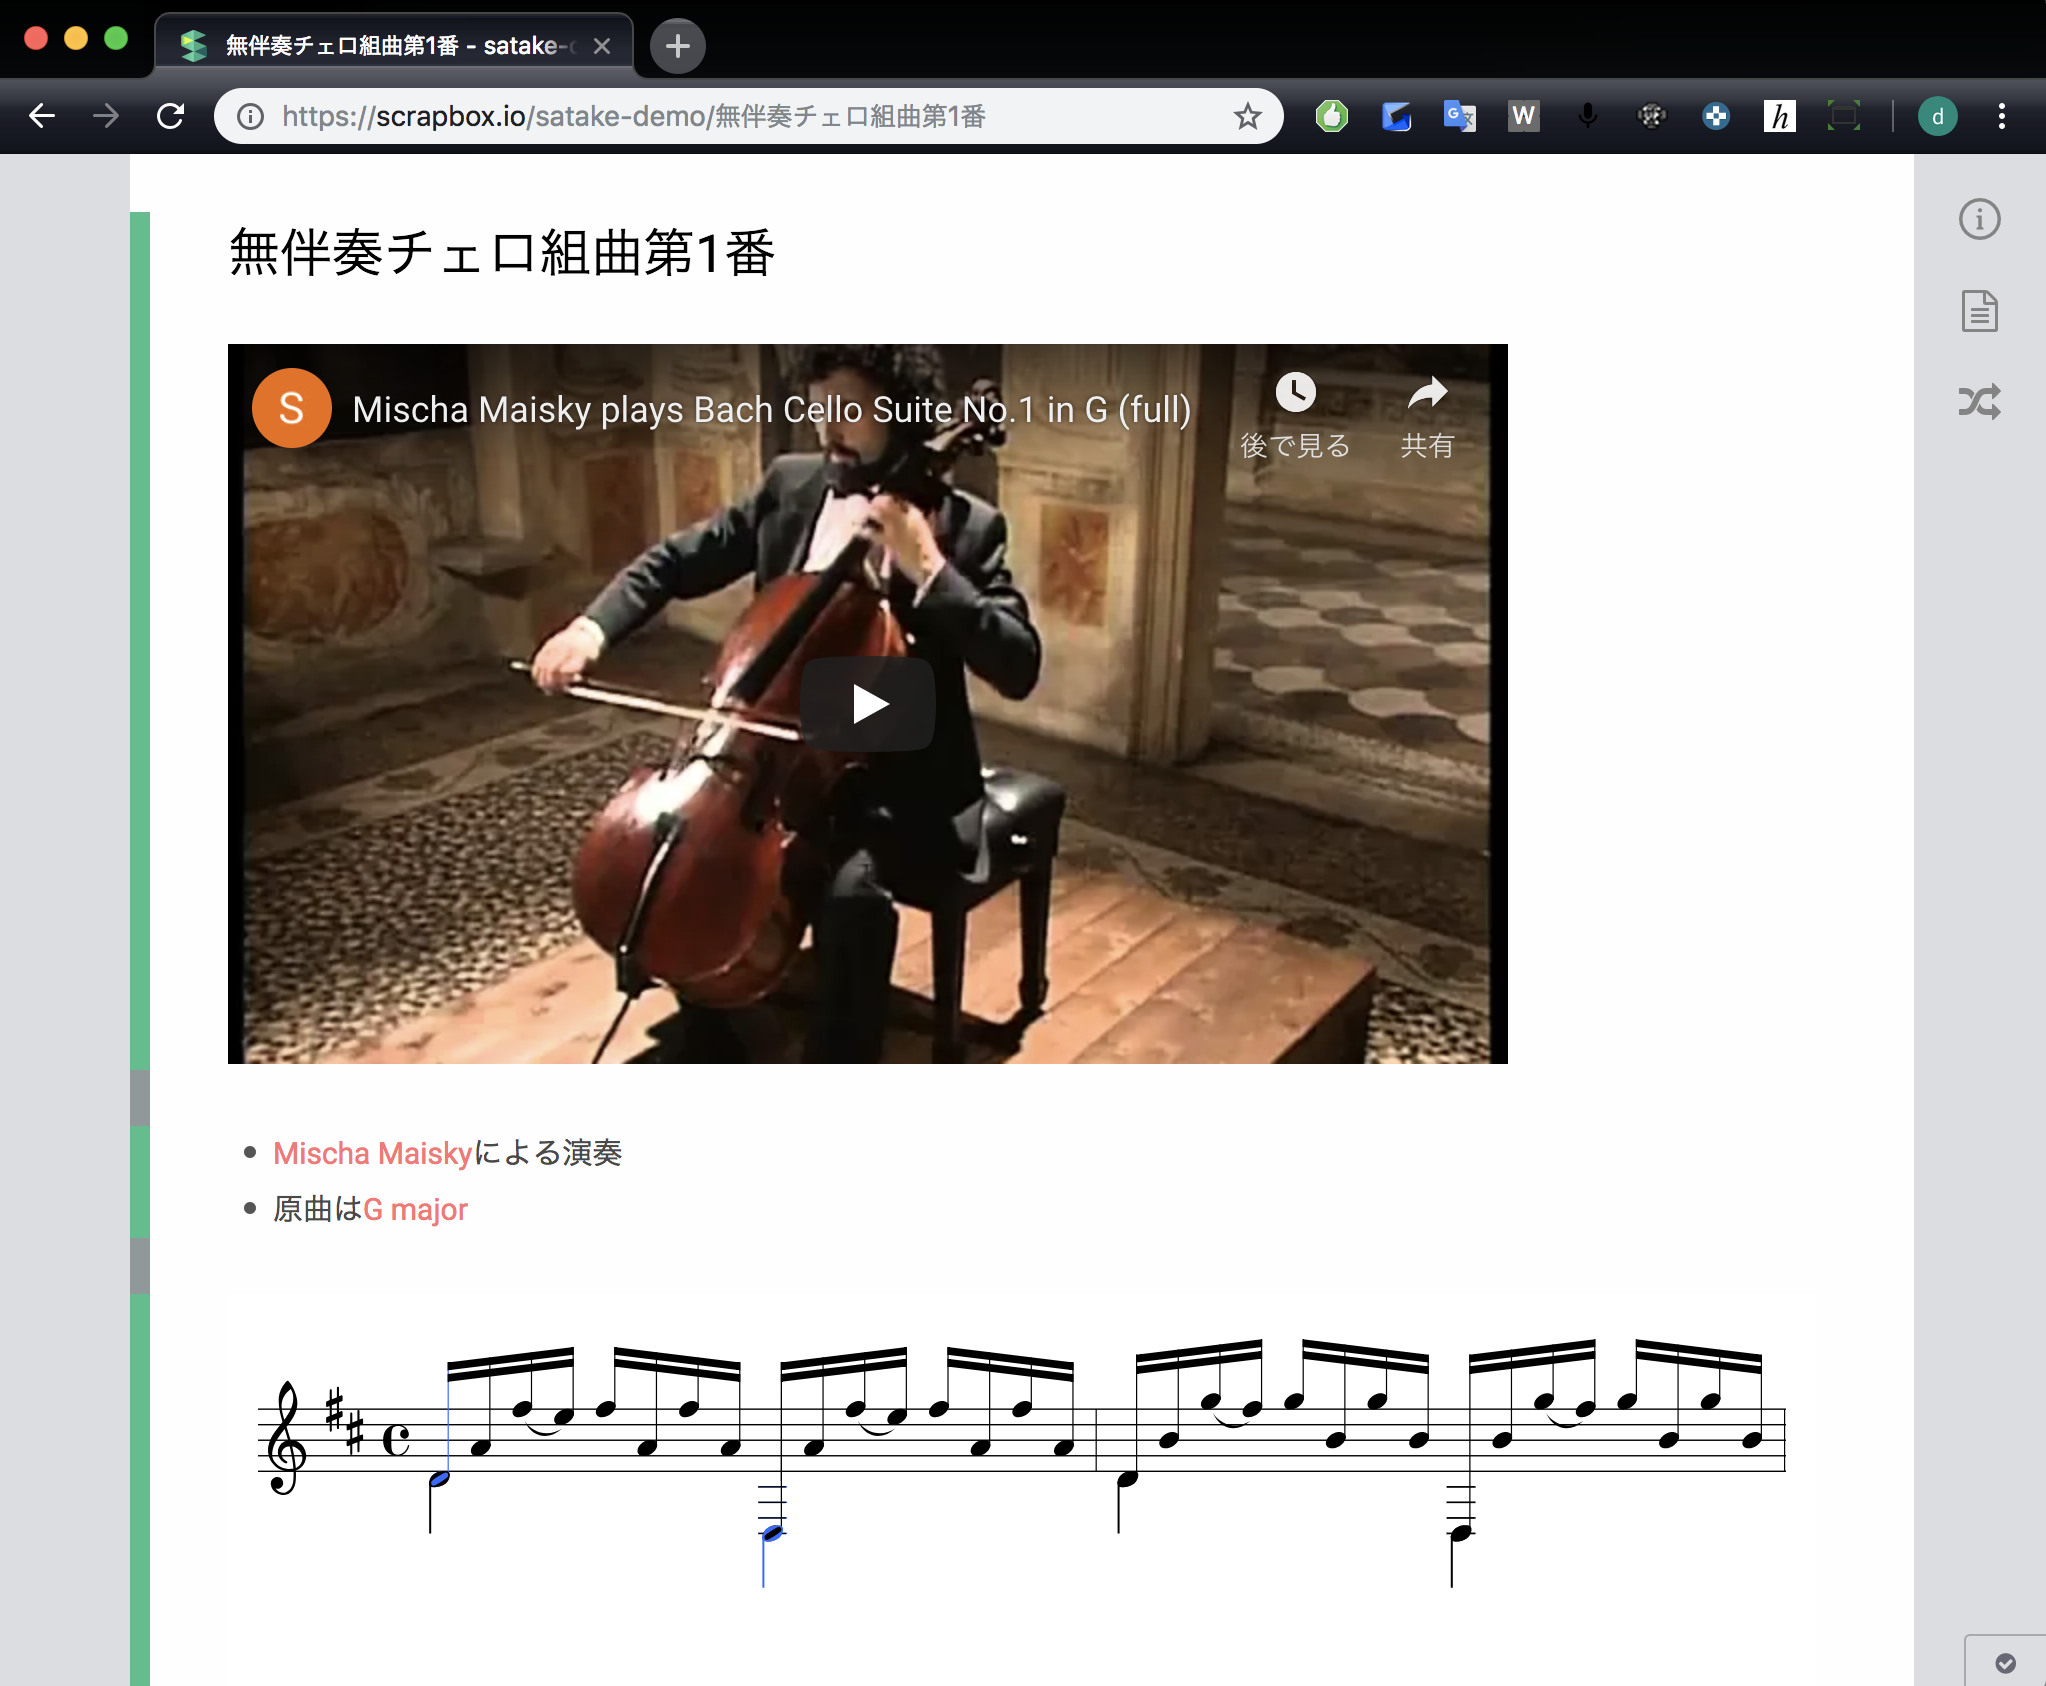
\includegraphics[width=10cm]{images/scoreandtext.png}
\caption{楽譜にテキストや動画が埋め込まれた例}
\label{scoreandtext}
\end{figure}


\paragraph*{ハイパーリンクを利用する}
ABCには無い独自の機能として音符ハイパーリンク機能を利用できる。
ABCの末尾に\texttt{\%Links:[リンク1][リンク2]…}と記述することで対象となる音符にハイパーリンクを設定できる。
具体的な設定方法とその例を図\ref{linkabc}に示す。
ハイパーリンクが設定された音符は青く表示され(図\ref{linkednote})、クリックするとリンク先のページへ遷移する(図\ref{middlec})。

\begin{figure}[H]
\centering
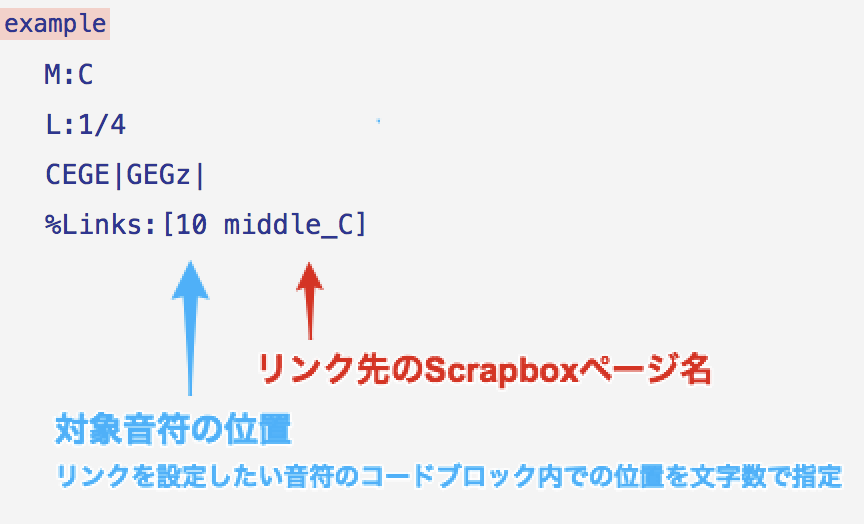
\includegraphics[width=10cm]{images/linkabc.png}
\caption{1音目の「C」に「middle C」ページへのリンクが設定されたABC}
\label{linkabc}
\end{figure}

\begin{figure}[H]
\centering
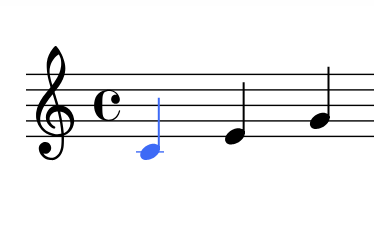
\includegraphics[width=4cm]{images/linkednote.png}
\caption{ハイパーリンクが設定された音符}
\label{linkednote}
\end{figure}

\begin{figure}[H]
\centering
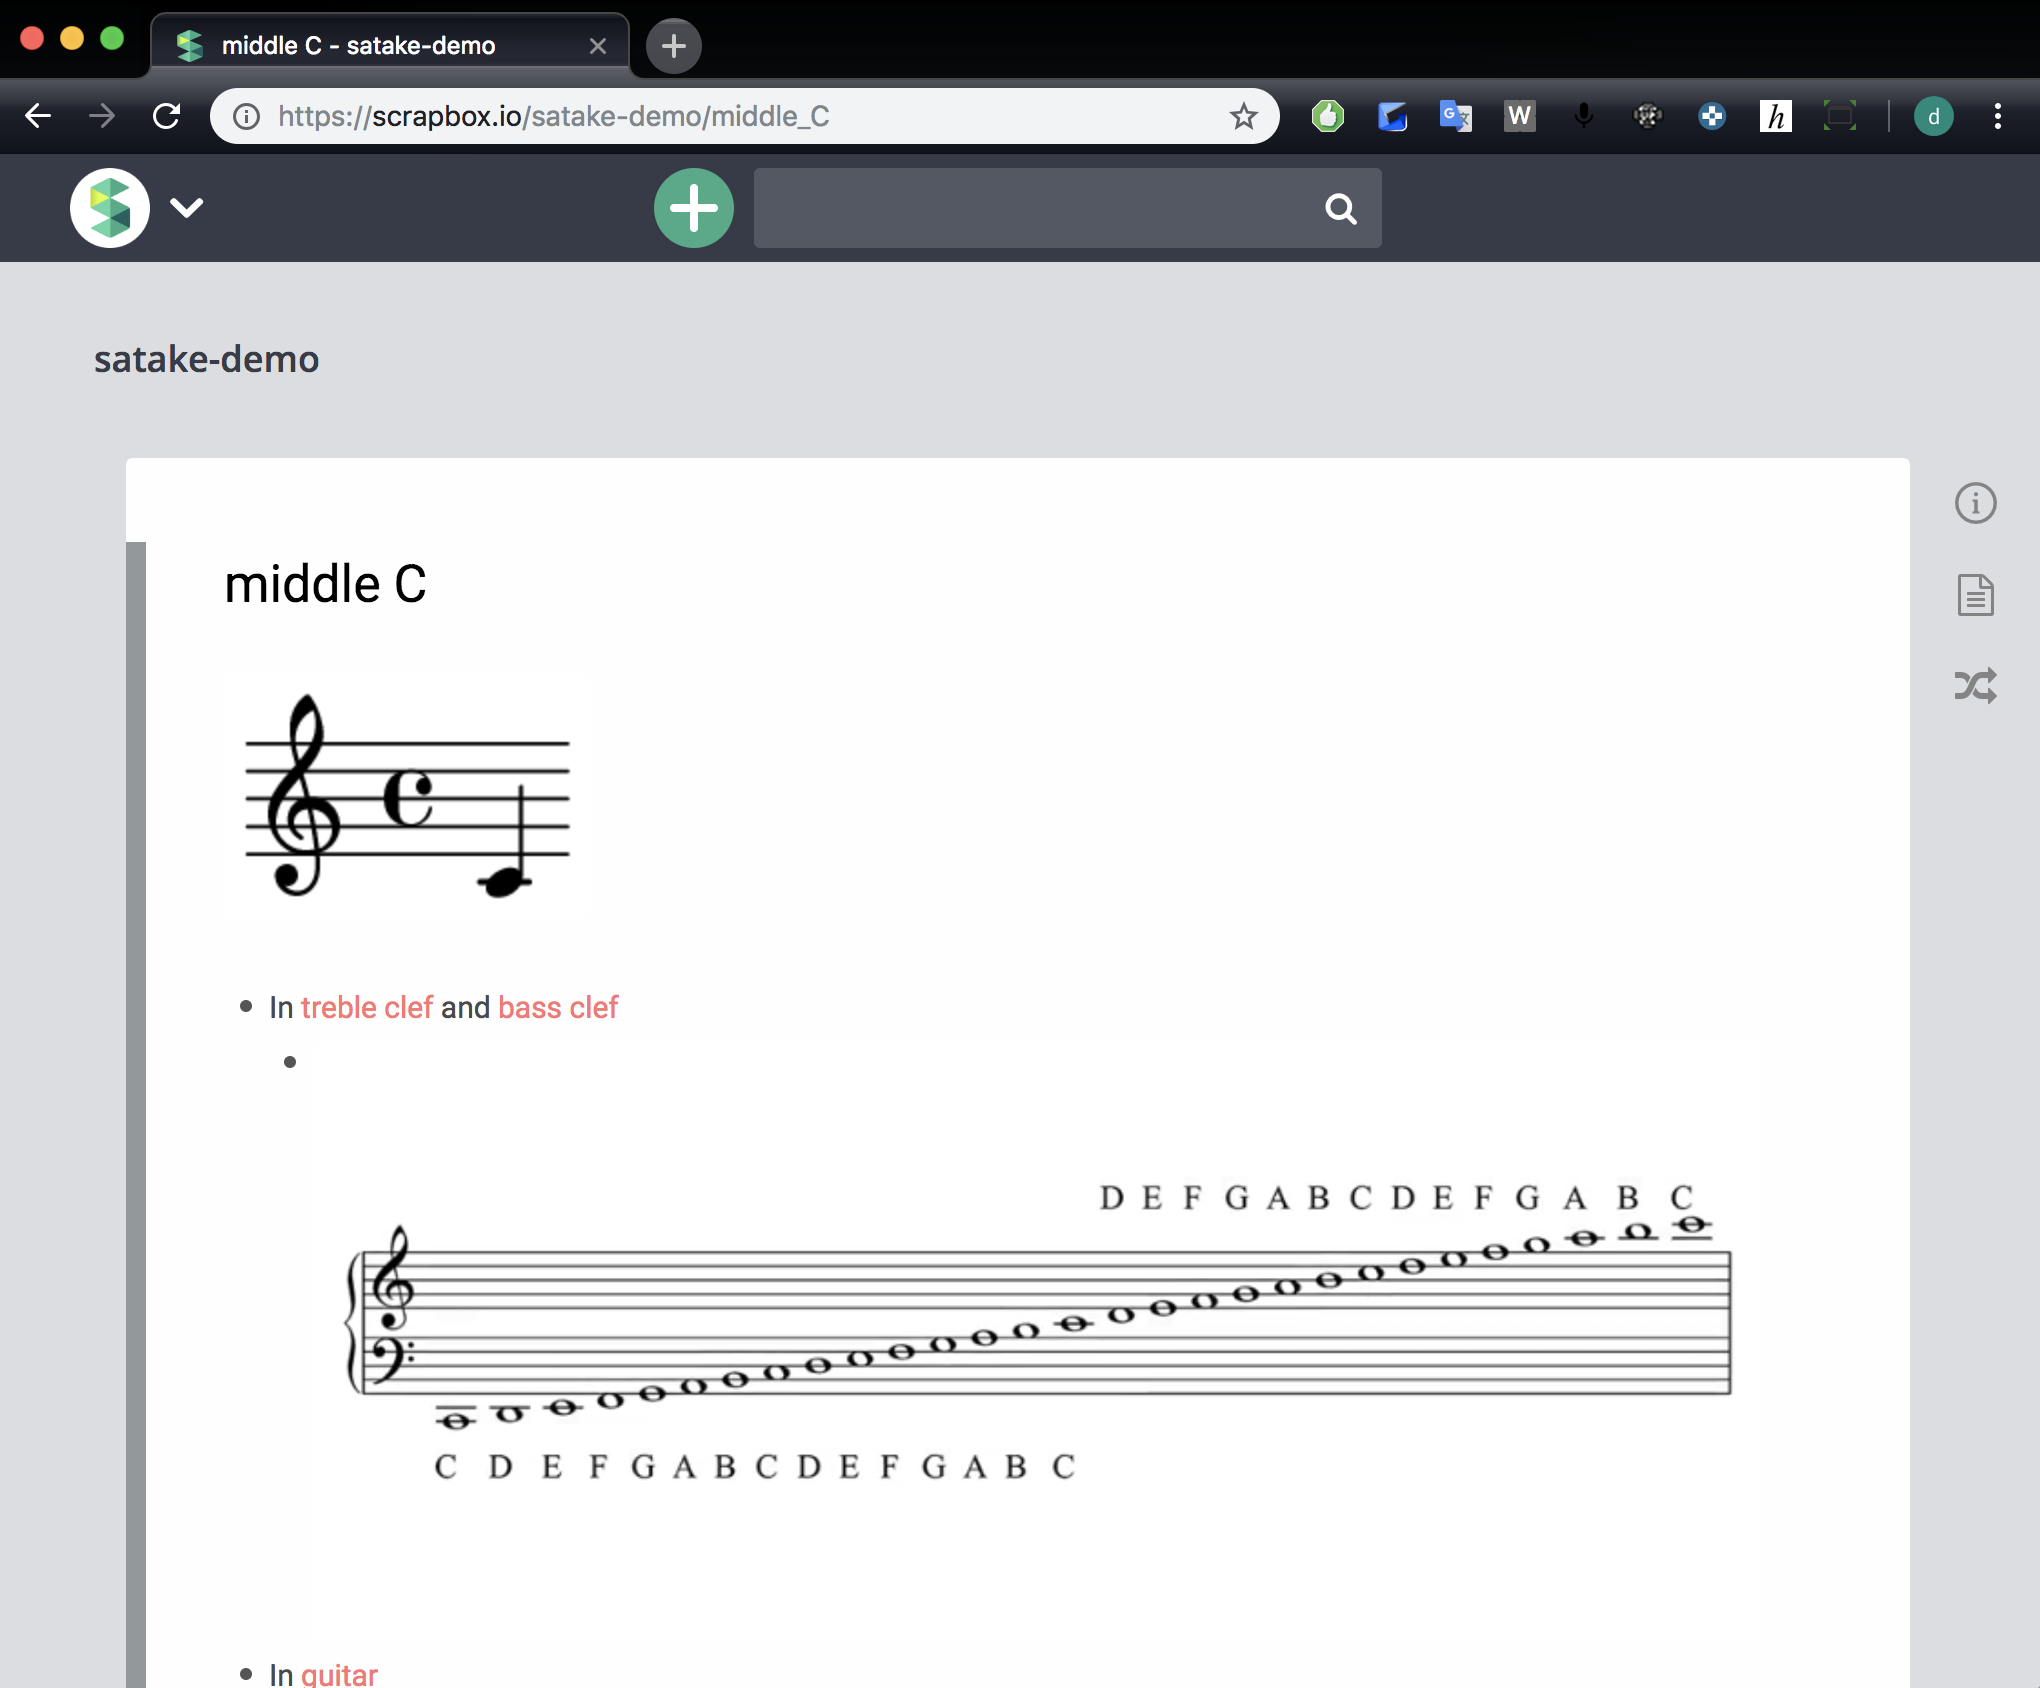
\includegraphics[width=10cm]{images/middlec.png}
\caption{リンク先の「middle C」ページ}
\label{middlec}
\end{figure}

  % 本文3
\chapter{実装}
\label{chap:jissou}

本章では第\ref{chap:sekkei}章で述べたシステムの設計を受け、ハイパー楽譜システムの実装について述べる。

\newpage

\section{アプリケーション構成}
ハイパー楽譜システムはScrapbox上で利用するChrome Extensionとして実装されている\footnote{\textsf{https://chrome.google.com/webstore/detail/hyperscorebox/cjlhoobllhkpjjomlijlfdblgifcdmoh}}。
Chrome Extensionをインストール可能なPC版Google Chromeを利用できる環境であれば、OSを問わず利用することができる。
Chrome Extensionの開発にはTypeScript\footnote{\textsf{https://www.typescriptlang.org/}}を、楽譜の出力にはabcjsを利用している。
%以下に本システムの構成図を示す。
%イラストでも書く

\paragraph*{Chrome Extension}
Chrome ExtensionはGoogle Chrome上にインストール可能なブラウザの機能を拡張できるアプリケーションである。
一般的なWebページと同様に、HTML/CSS/JavaScriptのようなWeb技術を用いて実装することができ、
\begin{itemize}
    \item HTML要素の操作
    \item カスタムCSSの適用
    \item HTTPリクエスト
    \item 外部サービスとの連携
\end{itemize}といった機能が実現可能である。
アプリケーションはChrome Web Store\footnote{\textsf{https://chrome.google.com/webstore/category/extensions?hl=ja}}を通じて簡単に公開できる。

\section{楽譜の描画}
本節では楽譜描画の仕組みを述べる。

Scrapboxにはコードハイライトを行うコードブロック記法(図\ref{codeblock})が存在し、\texttt{"code:{ファイル名}"}と入力することで利用できる。
本アプリケーションではABCの記述にこのコードブロックを利用している。
本アプリケーションによってファイル名の拡張子が\texttt{*.abc}に一致するコードブロック(図\ref{abcblock})のみがABCとして解釈され、abcjsによって生成された楽譜画像(図\ref{cde})がコードブロックのHTML要素に対して重畳表示される。

\begin{figure}[H]
    \centering
    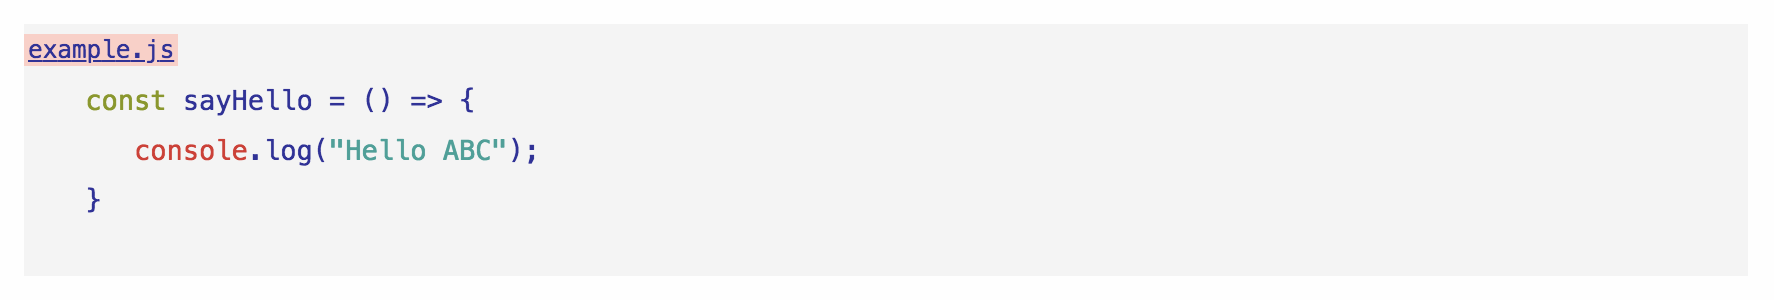
\includegraphics[width=15cm]{images/codeblock.png}
    \caption{コードブロック記法}
    \label{codeblock}
\end{figure}

\begin{figure}[H]
    \centering
    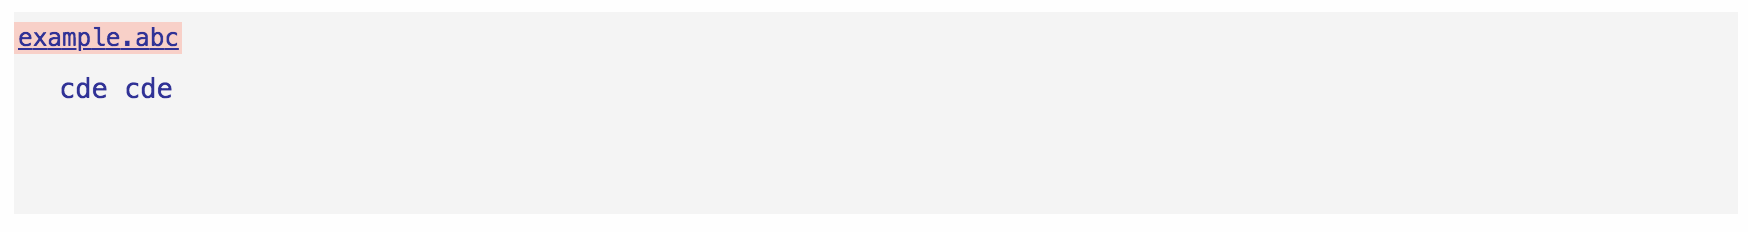
\includegraphics[width=15cm]{images/abcblock.png}
    \caption{ABCとして解釈されるコードブロック}
    \label{abcblock}
\end{figure}

\begin{figure}[H]
    \centering
    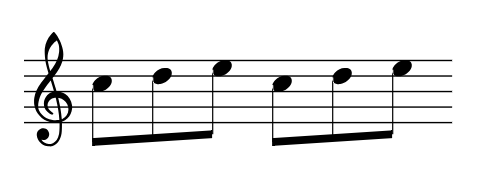
\includegraphics[width=5cm]{images/cdecde.png}
    \caption{生成された楽譜画像}
    \label{cde}
\end{figure}

\section{音符ハイパーリンク機能の実現}
本節では音符ハイパーリンク機能の実現方法を述べる。

abcjsはSVG画像として楽譜を出力しており、一つ一つの音符に対してクリックリスナを設定可能である。
\texttt{Document.location.href}オブジェクト\footnote{\textsf{https://developer.mozilla.org/ja/docs/Web/API/Location}}を利用してページ遷移を実行するコールバック関数を音符のクリックリスナに設定している。
  % 本文4
\chapter{楽譜IME}
\label{chap:ime}

本章では楽譜入力を支援する楽譜IMEを提案する。

\newpage

\section{ABCの問題点}
前章までに提案したハイパー楽譜システムでは、Wiki上での楽譜入力を実現するために、テキストベースでの楽譜記述を可能とするABCを利用している。
ABCはシンプルだが、
\begin{enumerate}
    \item 記法を覚える必要がある
    \item WYSIWYGでない
\end{enumerate}という問題点が存在する。
このうち2.はハイパー楽譜システムのリアルタイムな楽譜描画によって解決されている。
1.の解決には、文字変換を行う日本語入力システム(IME)的アプローチが有効であると考えられる。
本章では楽譜IMEを提案し、既存システムと比較しても遜色ない快適な楽譜入力を実現する。

\section{楽譜IME}
楽譜IMEは楽譜辞書を利用した変換機能によりABC特有の記法や様々な楽譜の入力をサポートする。
これは前章で実装したハイパー楽譜システムの一部として利用できる。
本節では主な機能や利用フローを解説する。

\subsection{利用できる機能}
\begin{enumerate}
    \item ABC入力支援機能
    \begin{itemize}
        \item ドレミ変換機能\\
        「ドレミ」のようなカタカナ音名をABCに変換する。ABCで利用される英語音名に慣れていなくても楽譜入力が可能になる。
        \item 記号変換機能\\
        「 $\sharp\;\;\flat\;\;\natural$ 」といった臨時記号をABCに変換する。ABCでは $\sharp\;\;\flat\;\;\natural$ をそれぞれ \verb|^ _ =| と表記するが、見慣れた記号をそのまま利用できることで、感覚的な入力が可能になる。
        \item オクターブ変更機能\\
        上下キーによって音符のオクターブを変更する。ABCではオクターブ上を\texttt{'}、下を\texttt{,}と表記するが、矢印キーを利用することで感覚的な入力が可能になる。
        \item MIDIデバイス入力機能\\
        MIDIキーボードといったデバイスから直接音符を入力する。
        既存の楽譜作成ソフトでは一般的な機能であり、鍵盤を利用することで感覚的な入力が可能になる。
    \end{itemize}
    \item 楽譜入力支援機能\\
    楽譜辞書を利用した変換機能によって楽譜の入力を支援する。
    例えばCメジャーの和音(ドミソ)を入力したいときは、\texttt{C}と入力するだけで変換が可能になる。
    ABCでは和音を入力するとき\texttt{[ceg]}のように構成音を全て記述する必要があるが、よく使う三和音などはその名前から変換できるようにすることで、楽譜入力の手間を軽減する。
\end{enumerate}

\subsection{利用フロー}
\begin{enumerate}
    \item 楽譜IMEの起動\\
    コードブロック内で\mbox{Esc}キーを押すと楽譜IMEが起動する(図\ref{ime})。
    \item 文字入力\\
    文字入力すると、入力中のABCテキストからリアルタイムに楽譜がプレビューされる(図\ref{candidate})。
    変換候補も同様に楽譜として表示される。
    ここでは\texttt{"C"}という入力に対して、Cメジャー、Cマイナーの和音が候補として提示されている。
    \item 変換候補の選択\\
    文字入力中にSpaceキーを押すと変換候補を選択できる(図\ref{select})。
    \item 変換候補の入力\\
    変換候補を選択した状態でEnterキーを押すと、その楽譜を入力できる(図\ref{input})。
\end{enumerate}

\begin{figure}[H]
    \centering
    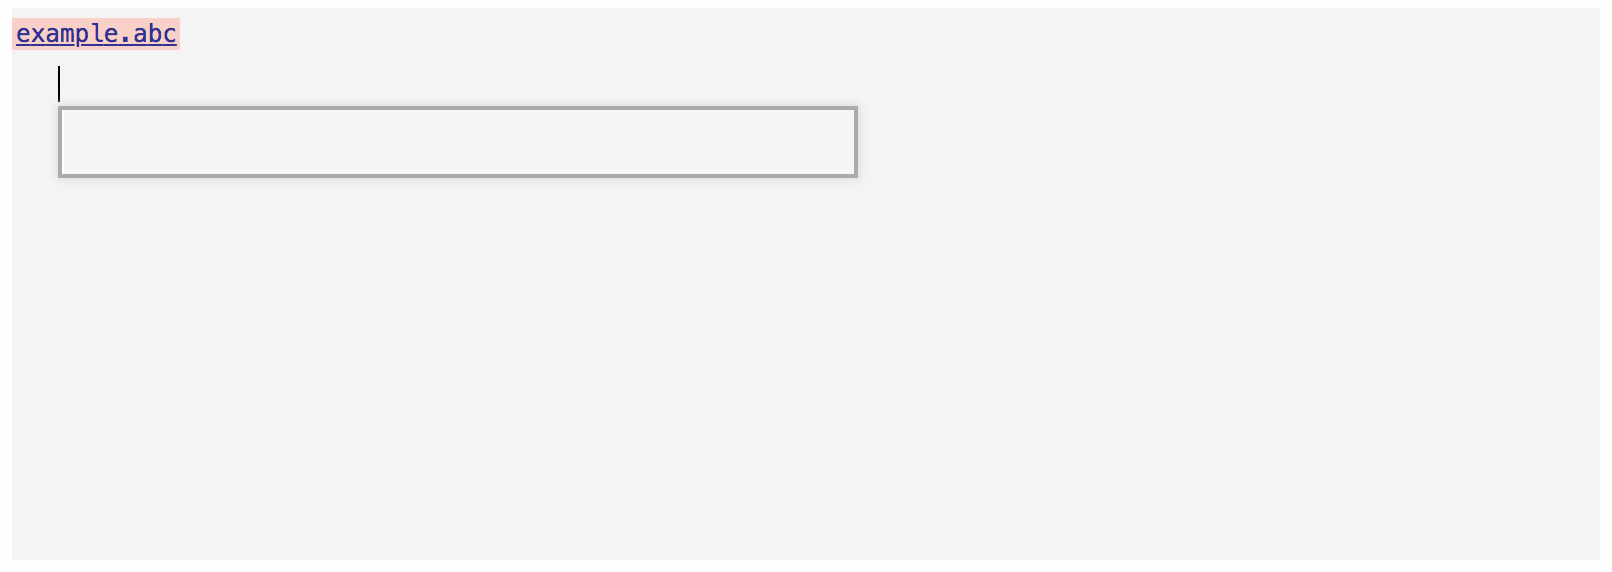
\includegraphics[width=13cm]{images/ime.png}
    \caption{楽譜IME初期画面}
    \label{ime}
\end{figure}

\begin{figure}[H]
    \centering
    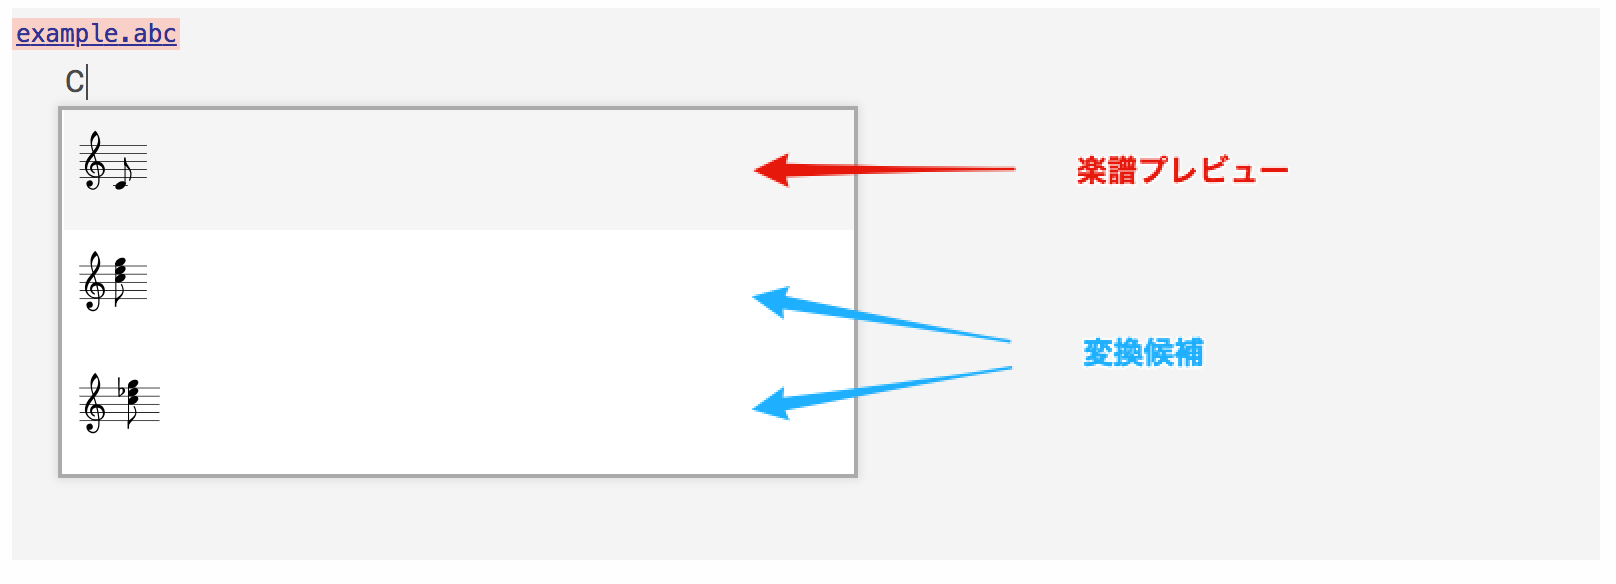
\includegraphics[width=13cm]{images/imecandidate.png}
    \caption{文字入力中の画面}
    \label{candidate}
\end{figure}

\begin{figure}[H]
    \centering
    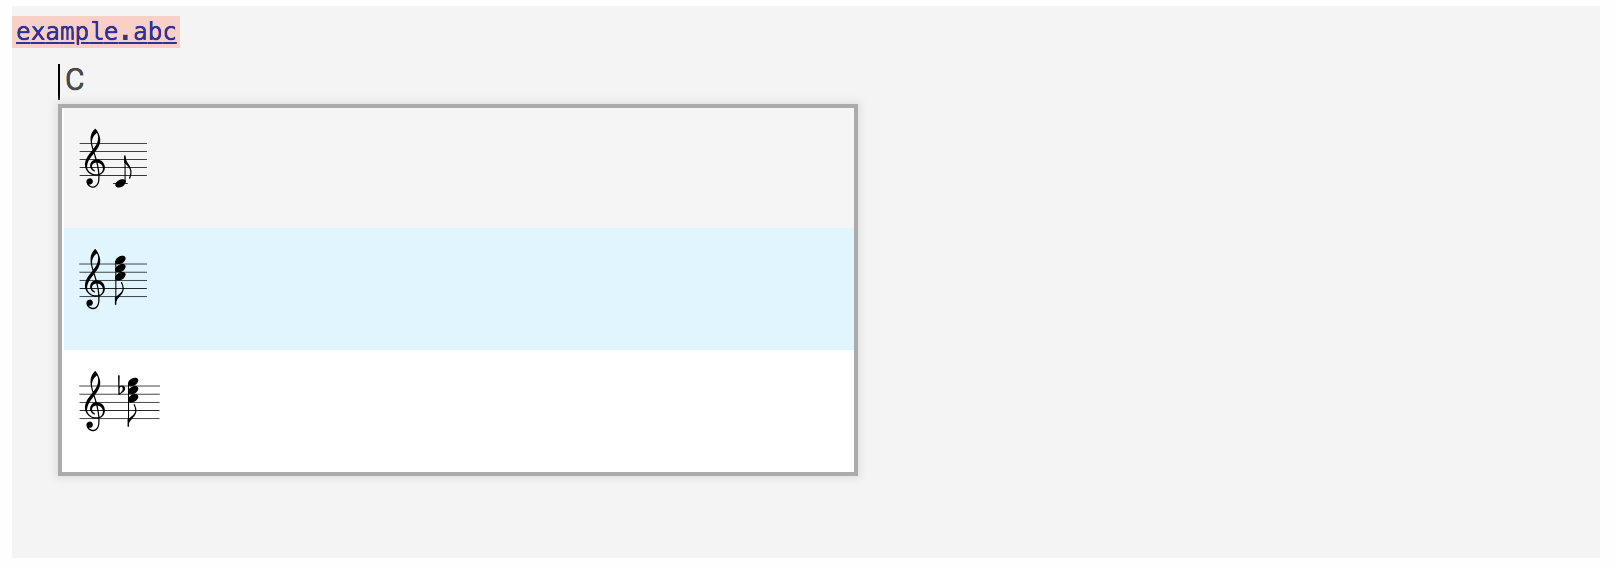
\includegraphics[width=13cm]{images/selectcandidate.png}
    \caption{変換候補選択中の画面}
    \label{select}
\end{figure}

\begin{figure}[H]
    \centering
    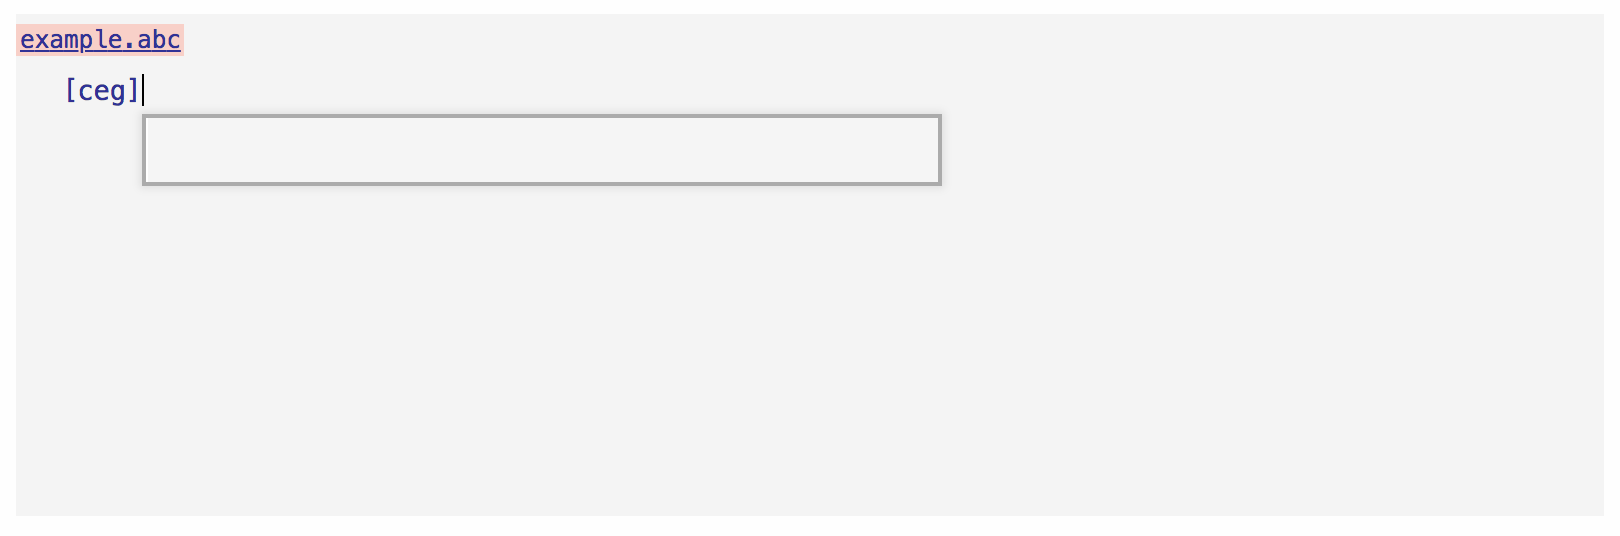
\includegraphics[width=13cm]{images/inputcandidate.png}
    \caption{変換が完了した画面}
    \label{input}
\end{figure}

\section{実装}
楽譜IMEはJavaScriptを用いてハイパー楽譜システムの内部に実装されており、ブラウザ上で利用可能である。本節では楽譜IMEのアプリケーション構成を解説する。

\subsection{文字入力}
楽譜IMEはOSから利用できるIMEとは異なり、アプリケーション自身がブラウザからキーイベントを取得する。
具体的には、ブラウザが発行するキー入力イベントがScrapboxに渡される前に横取りする形で受け取り、各種変換処理を実行している。
楽譜IME上で変換処理が確定されると、テキストエリア上の文章を操作する\texttt{Document.execCommand()}関数\footnote{\textsf{https://developer.mozilla.org/ja/docs/Web/API/Document/execCommand}}を利用してブラウザに文字入力を指示する。

\subsection{楽譜の表示}
楽譜IME起動時は楽譜プレビュー・変換候補表示用のDiv要素をScrapboxの画面上に重畳表示し、ハイパー楽譜システム同様abcjsを用いて楽譜を描画している。

\subsection{楽譜辞書}
辞書データはソースコード\ref{dict}のようなJSON形式で保持している。
辞書エントリの第1要素は楽譜の読み、第2要素は変換されるABCテキストを示している。
このような構造は既存の日本語入力システム\cite{Masui}と同様のものである。
\begin{lstlisting}[caption=楽譜IMEの辞書データ, label=dict]
[
    ["C", "[ceg]"],
    ["Cm", "[c_eg]"],
    …
]
\end{lstlisting}


\section{議論}
本節では楽譜IMEの利用において気付いた点などを述べる。
\subsection{使用感}
楽譜IMEは既存のIMEと同様のインターフェースを提供しており、入力の対象が楽譜となっても候補が表示されたり候補を選択したりする感覚は共通であることから、快適に楽譜を入力できた。
一方で、楽譜辞書のエントリ数が少ないため、思うような変換ができない場面もあった。

\subsection{辞書の編集}
現在、楽譜IMEの辞書は筆者自身が編集している。
和音を中心にエントリを追加しているが、幅広いシーンで変換機能を利用するためには辞書の充実が求められる。
しかし、コードネームやスケールといった一般的な音楽知識でさえジャンルや文脈によって名前が異なることがあり、開発者1人で網羅的な辞書を作成するのは大変困難な作業である。
単語と楽譜が対応するような辞書は存在しないので、Lexierra\cite{Masui}のようにWiki上で辞書を編集する手法が有効であると考えられる。
Wikiを利用することでソーシャルに辞書を編集できるため、膨大なエントリを協力して編集したり、ユーザーそれぞれが必要なエントリを自由に追加するといったことが可能になる。
またScrapbox上で辞書を構築すればハイパー楽譜システム・楽譜IMEを利用できるため、効率的な楽譜辞書編集が可能となる。

\subsection{動的な辞書}
ページ内外の別の楽譜をそのまま利用したいシーンがあった。
コピー\verb|&|ペーストでも対応できるが、事前に用意した楽譜辞書だけでなく、Scrapboxプロジェクト内の楽譜から動的に辞書を構築できれば、より柔軟な楽譜入力が実現できると考えられる。
また前述のソーシャルな辞書編集環境が実現された場合、ユーザーそれぞれが必要なエントリを自由に追加できるが、あるユーザーにとっては不要なエントリが変換候補として提案されてしまう可能性がある。
用途に合わせて利用する辞書を切り替えたり、エントリを絞り込むことができれば解決できると考えられる。

\section{まとめ}
ハイパー楽譜システム上で利用可能な楽譜IMEを提案した。
日本語入力システムの仕組みをABCに適用し、楽譜辞書によってABC入力を支援するシステムを実現した。
Wikiによるソーシャルな辞書編集環境や動的な辞書を実装し、あらゆる楽譜入力シーンで利用できるIMEとして拡張を行っていく予定である。
\chapter{応用例}
\label{chap:ouyou}

本章では、ハイパー楽譜システムによって実現可能な応用例について述べる。

\newpage

\section{楽器練習}
楽器練習の際は気付いたこと・習ったことなどをメモしながら楽譜を使うのが一般的である。
しかし楽譜上でメモ可能な領域は限られており、自由に書くことはできない。
また楽譜は曲単位で独立しているのでメモした情報が各楽譜に散逸してしまったり、そもそもどこに書いたか分からなくなってしまう問題もある。
本システムではレイアウトの制約を受けず自在にメモを書いたり、技術要素毎にページ(図\ref{seja})を用意して情報を一元管理することができる。

\begin{figure}[H]
\centering
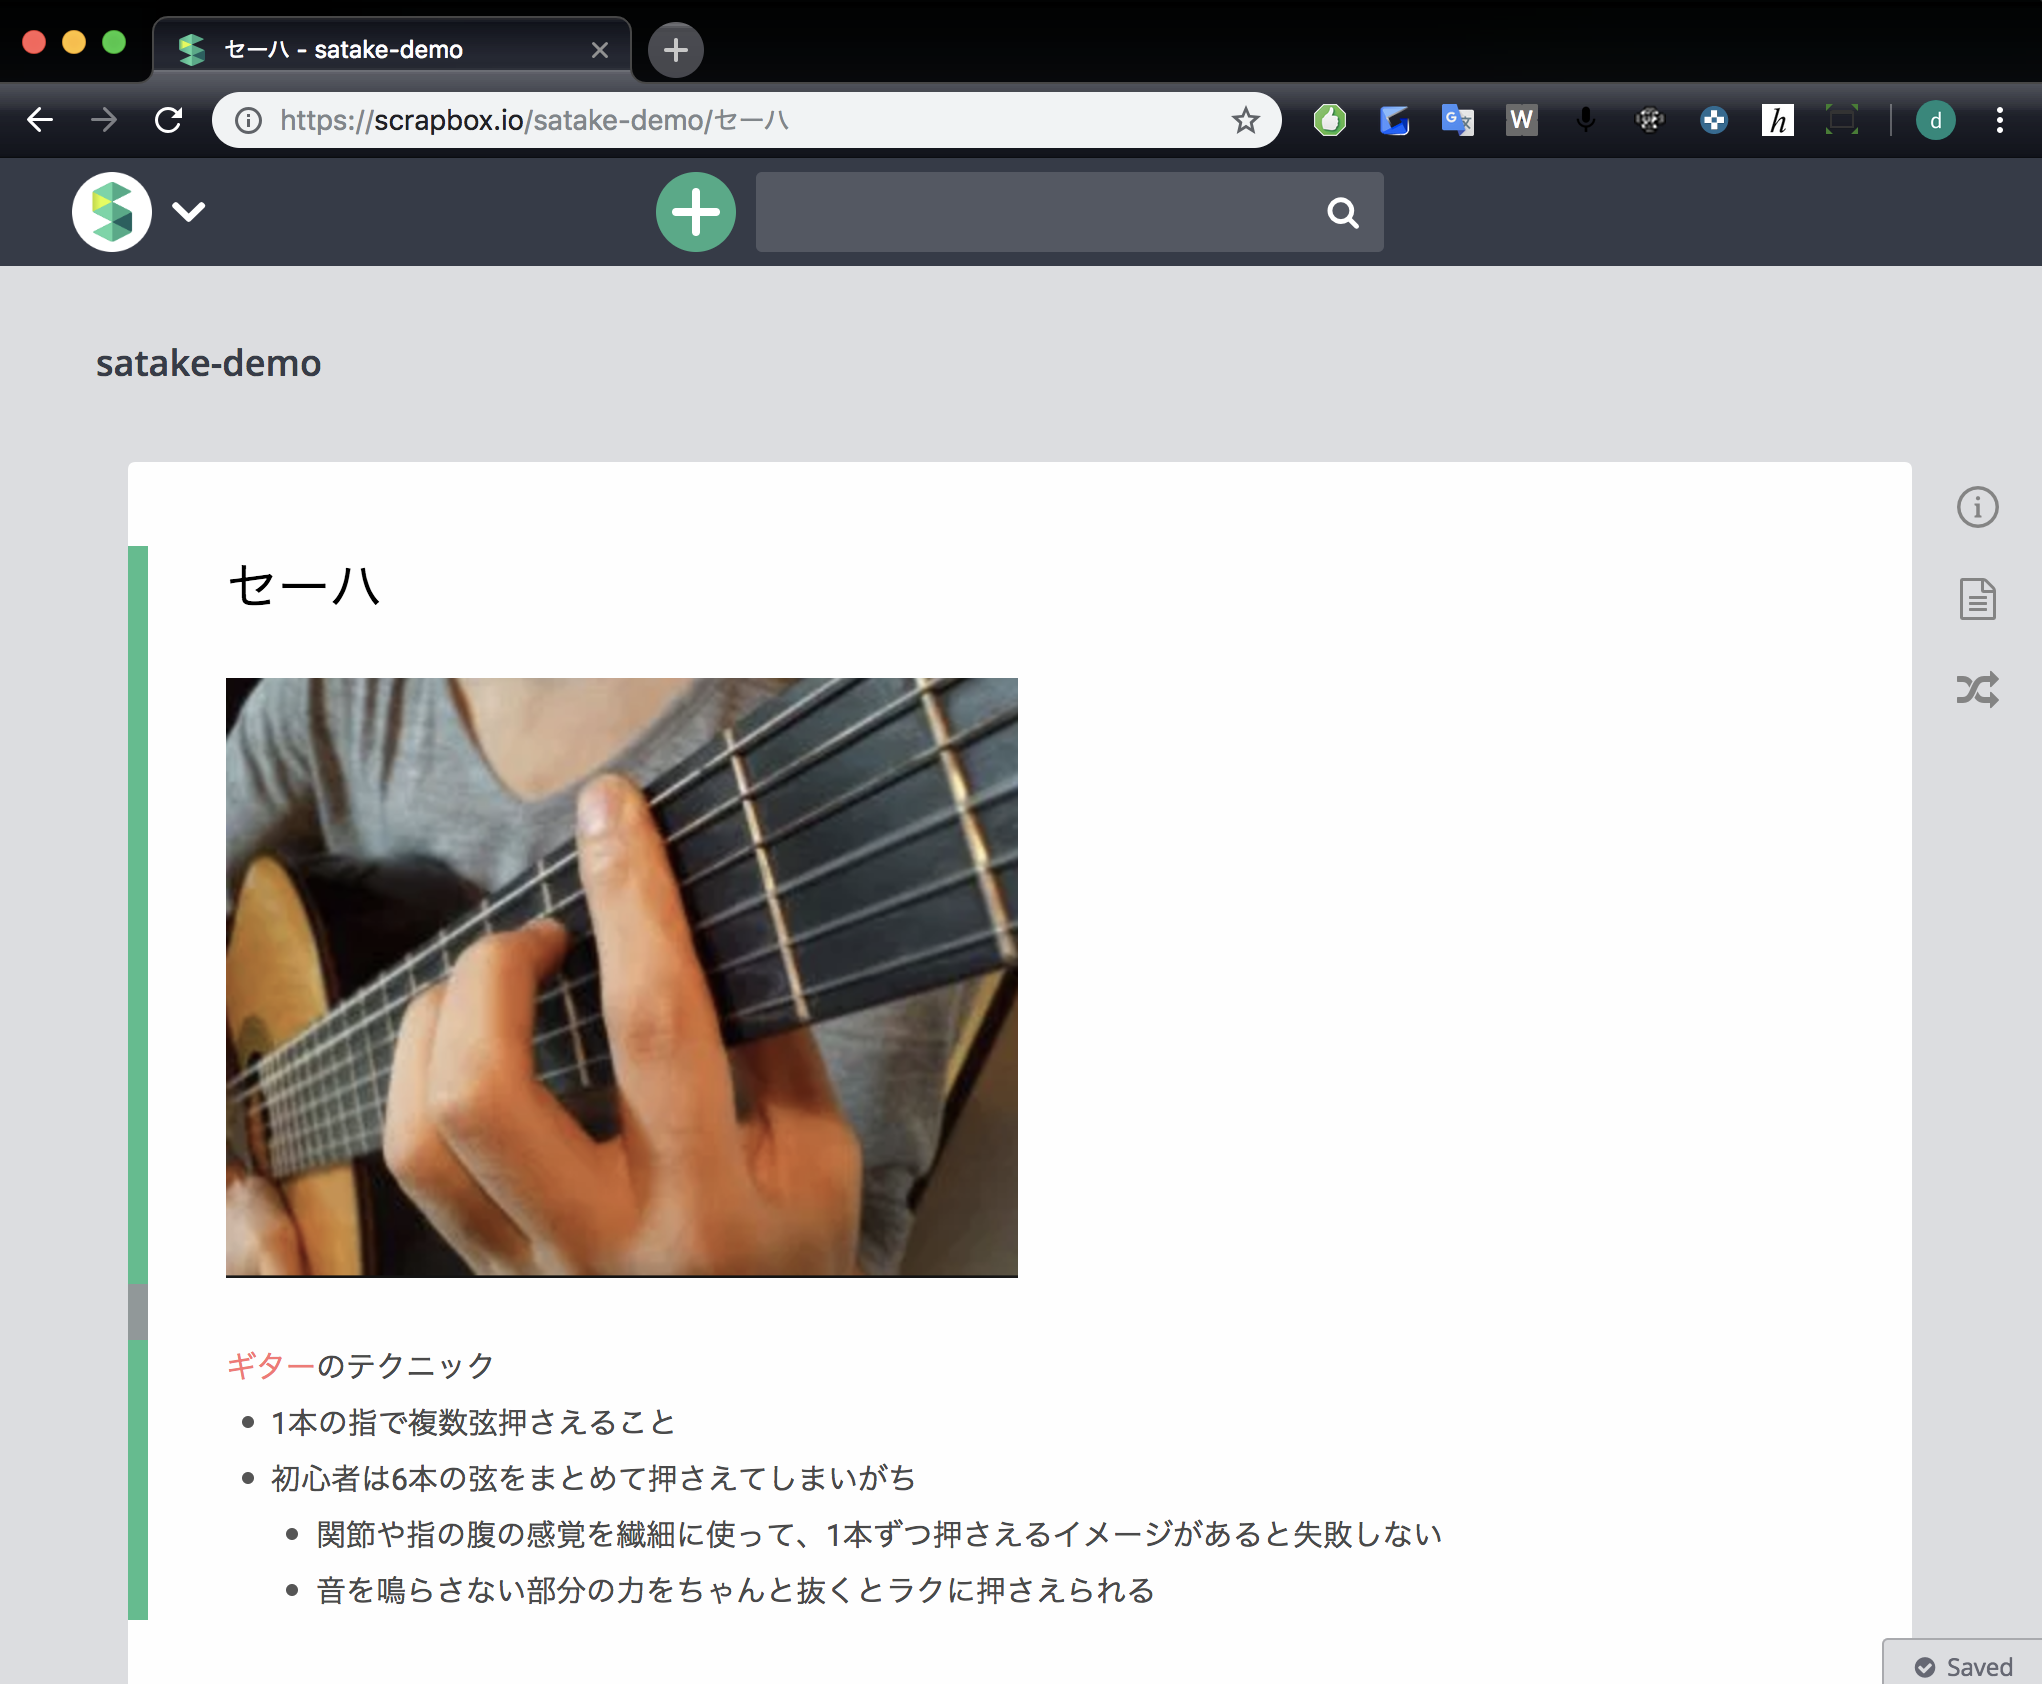
\includegraphics[width=10cm]{images/seja.png}
\caption{技術ページの例}
\label{seja}
\end{figure}

\section{勉強}
楽典や音楽理論といった知識は専門書のように楽譜とは独立した場所に書かれることが多く、学習者が関心のある楽曲との関連性を把握するのが難しい。
本システムでは、楽典や音楽理論といった知識を楽譜と同じScrapboxプロジェクトに記録しておく(図\ref{dominant})ことで、実際の楽曲と結びついた勉強環境を実現できる。
それぞれのページでは楽譜/テキスト/マルチメディアを用いて分かりやすく記述できるだけでなく、ハイパーリンクによって楽曲との関連性を可視化し、勉強/演奏をシームレスに繋げることができる。
そしてページが追加されるうちにたくさんの知識や楽曲がハイパーリンクで結びつき、Scrapboxプロジェクト全体が自分専用の教材として利用できるようになる。
本システムによって、楽譜とテキストのみで表現力が乏しい/実際の楽曲との関連が分からないといった既存の教材の問題点を解決しながら、勉強するだけで教材が作られていくという新しい勉強法を実現できる。

\begin{figure}[H]
\centering
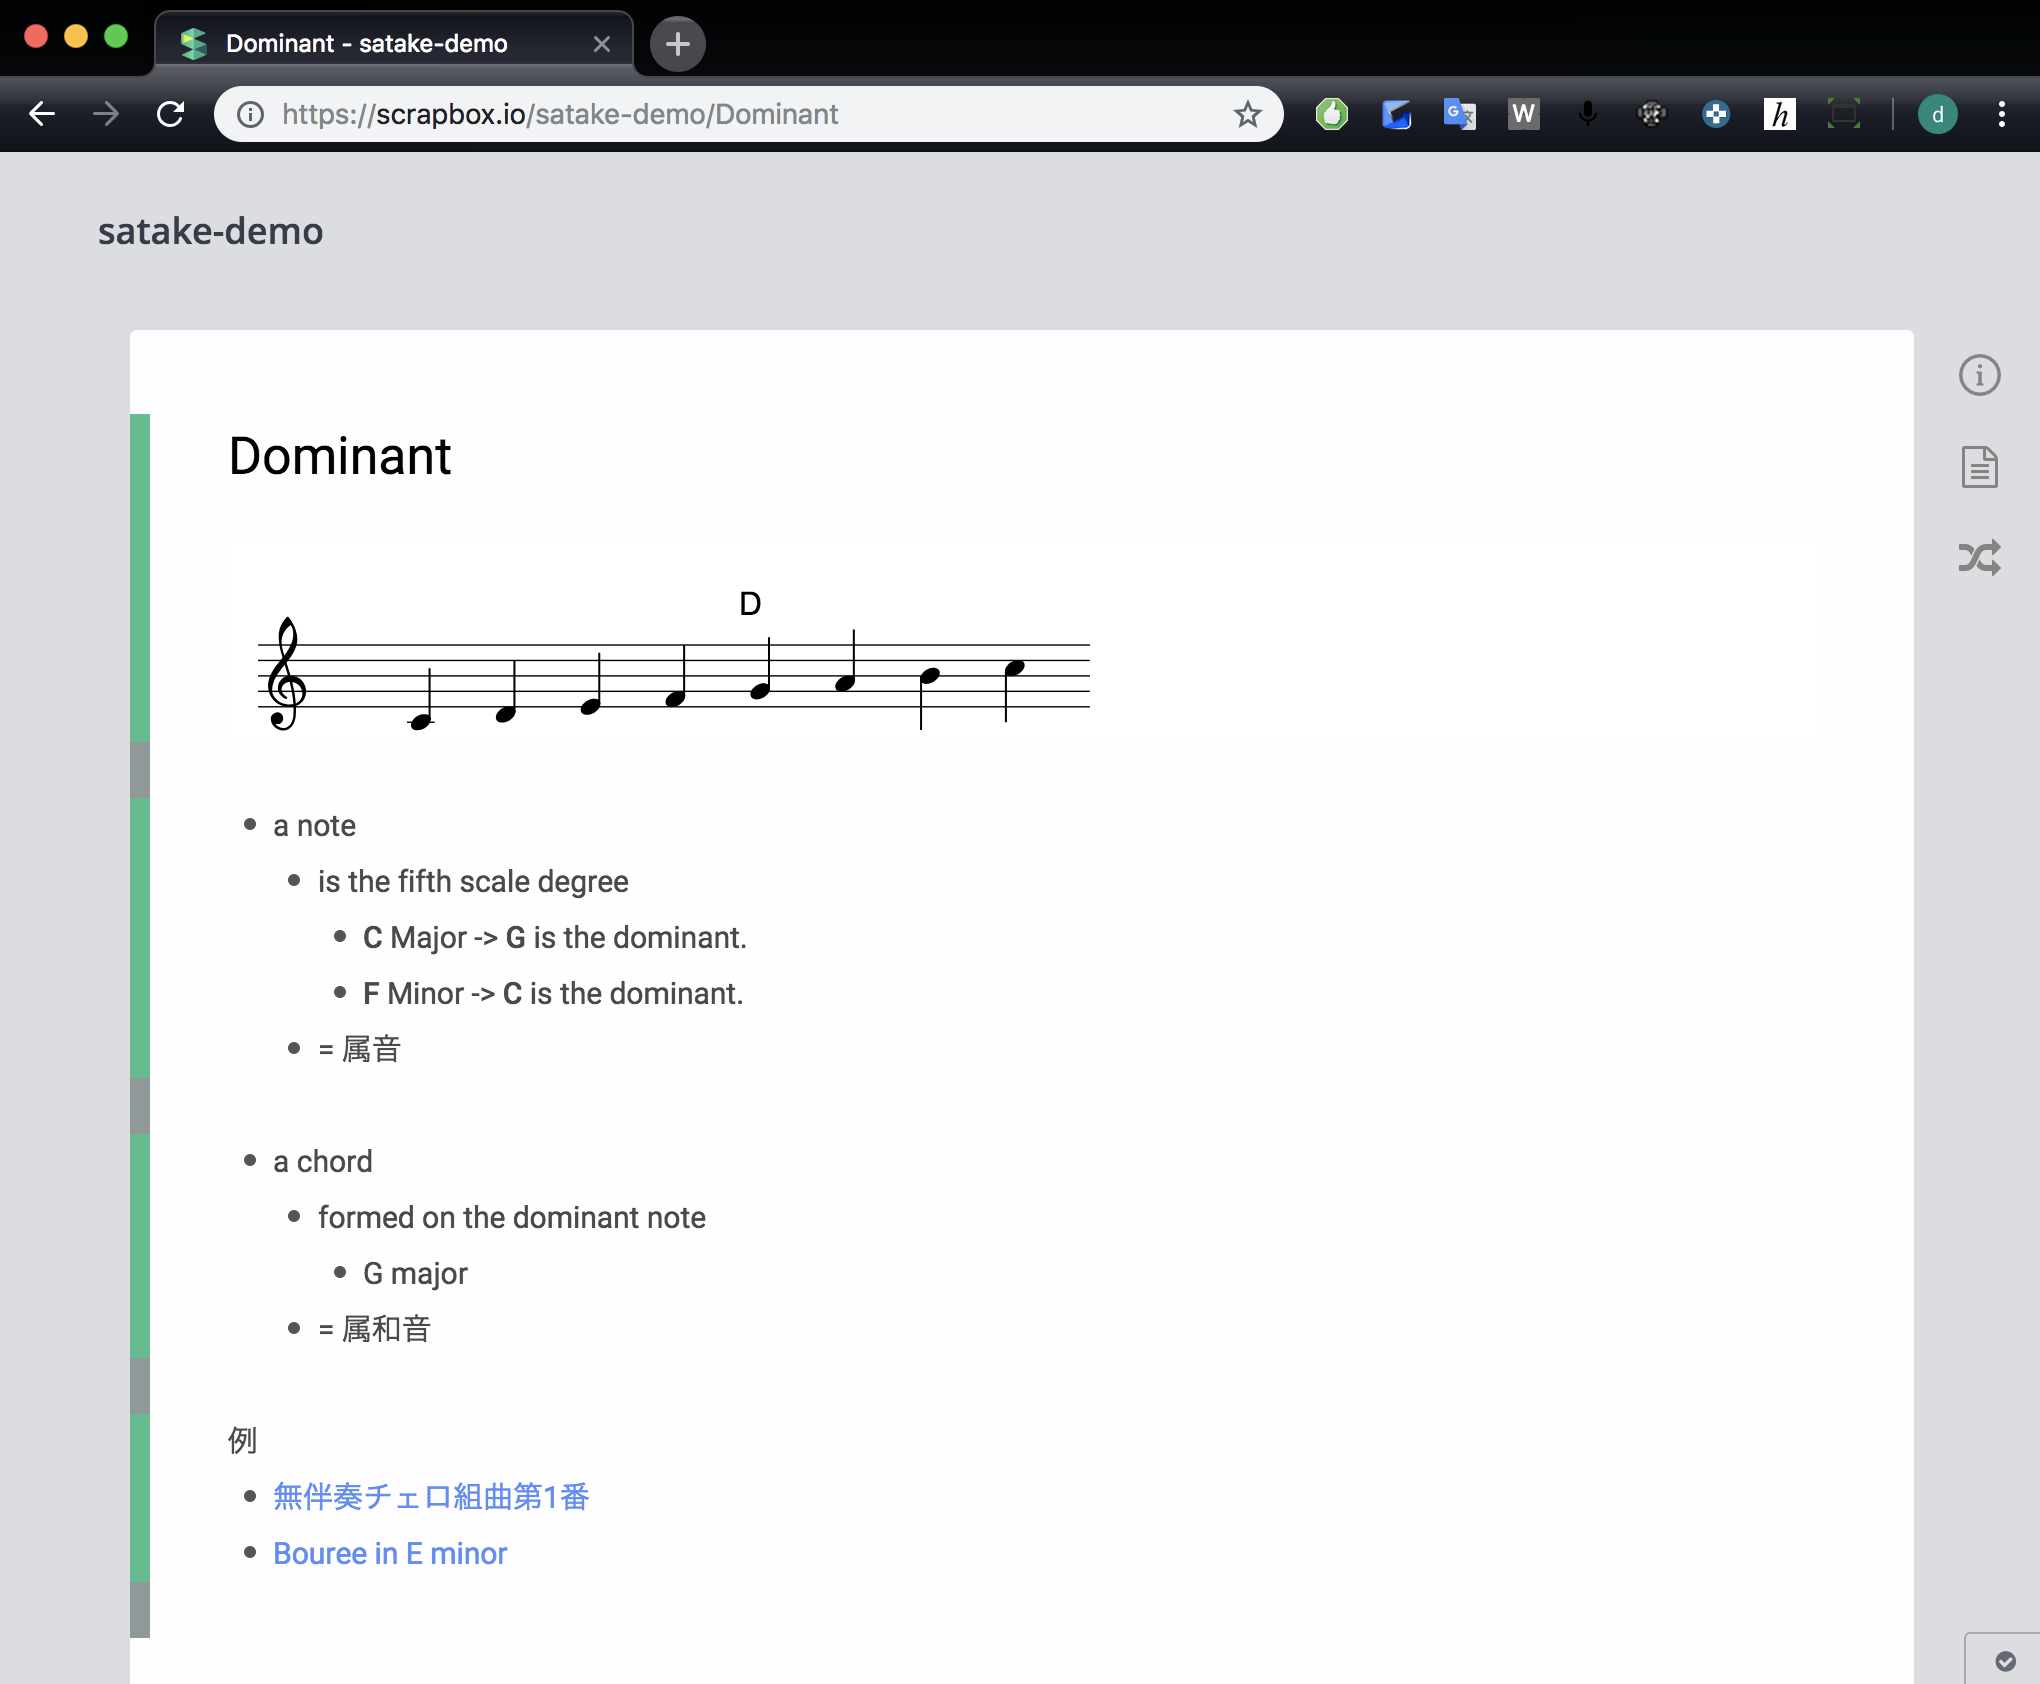
\includegraphics[width=10cm]{images/dominant.png}
\caption{知識ページの例}
\label{dominant}
\end{figure}

\section{楽譜共同編集}
本システムでは楽譜をテキストとして記述しているため、Scrapboxの強力な共同編集機能を活用し、柔軟な楽譜編集を実現できる。
例えば採譜(耳コピ)のような作業をパートや楽章毎に分担することで、大規模な楽譜でも一人一人の負担を軽減することができる。
作曲/編曲といった用途では、作者と演奏者が同じページ上で作業することで、楽譜の変更や演奏者のフィードバックを瞬時に共有することができる。

\section{楽曲の調査/分析}
筆者が所属する増井研究室ではあらゆる情報共有にScrapboxが利用されており、その中には研究に関する話題だけでなく、アニメや音楽といった趣味の情報も多く書かれている。
ハイパー楽譜システムの運用時に、あるアニメ主題歌のメロディやコード進行がとても独創的であったために研究室内で話題になり、Scrapbox上で情報収集や分析が行われるようになった。
その楽曲のページにはYouTube動画や音楽家による考察、作曲者自身のツイートなどがまとめられると同時に、ハイパー楽譜システムを活用して採譜が行われた(図\ref{aobuta})。
音やリズムが適切かというような議論を活発に行いながら楽譜が編集され、楽曲に対する理解が深まったと同時に、和気あいあいと議論しながら曲を分析するという音楽の楽しみ方を発見できた。

もしハイパー楽譜システムが存在しなければ採譜自体が行われなかったと考えられる。
Scrapbox上で楽譜を利用するには楽譜を画像化する必要があり変更が難しくなってしまうし、既存の楽譜作成システムは美しいレイアウトで清書するための環境なので、楽譜を試行錯誤しながら書いたり、断片的にメモ書きするような用途には適さない。

\begin{figure}[H]
\centering
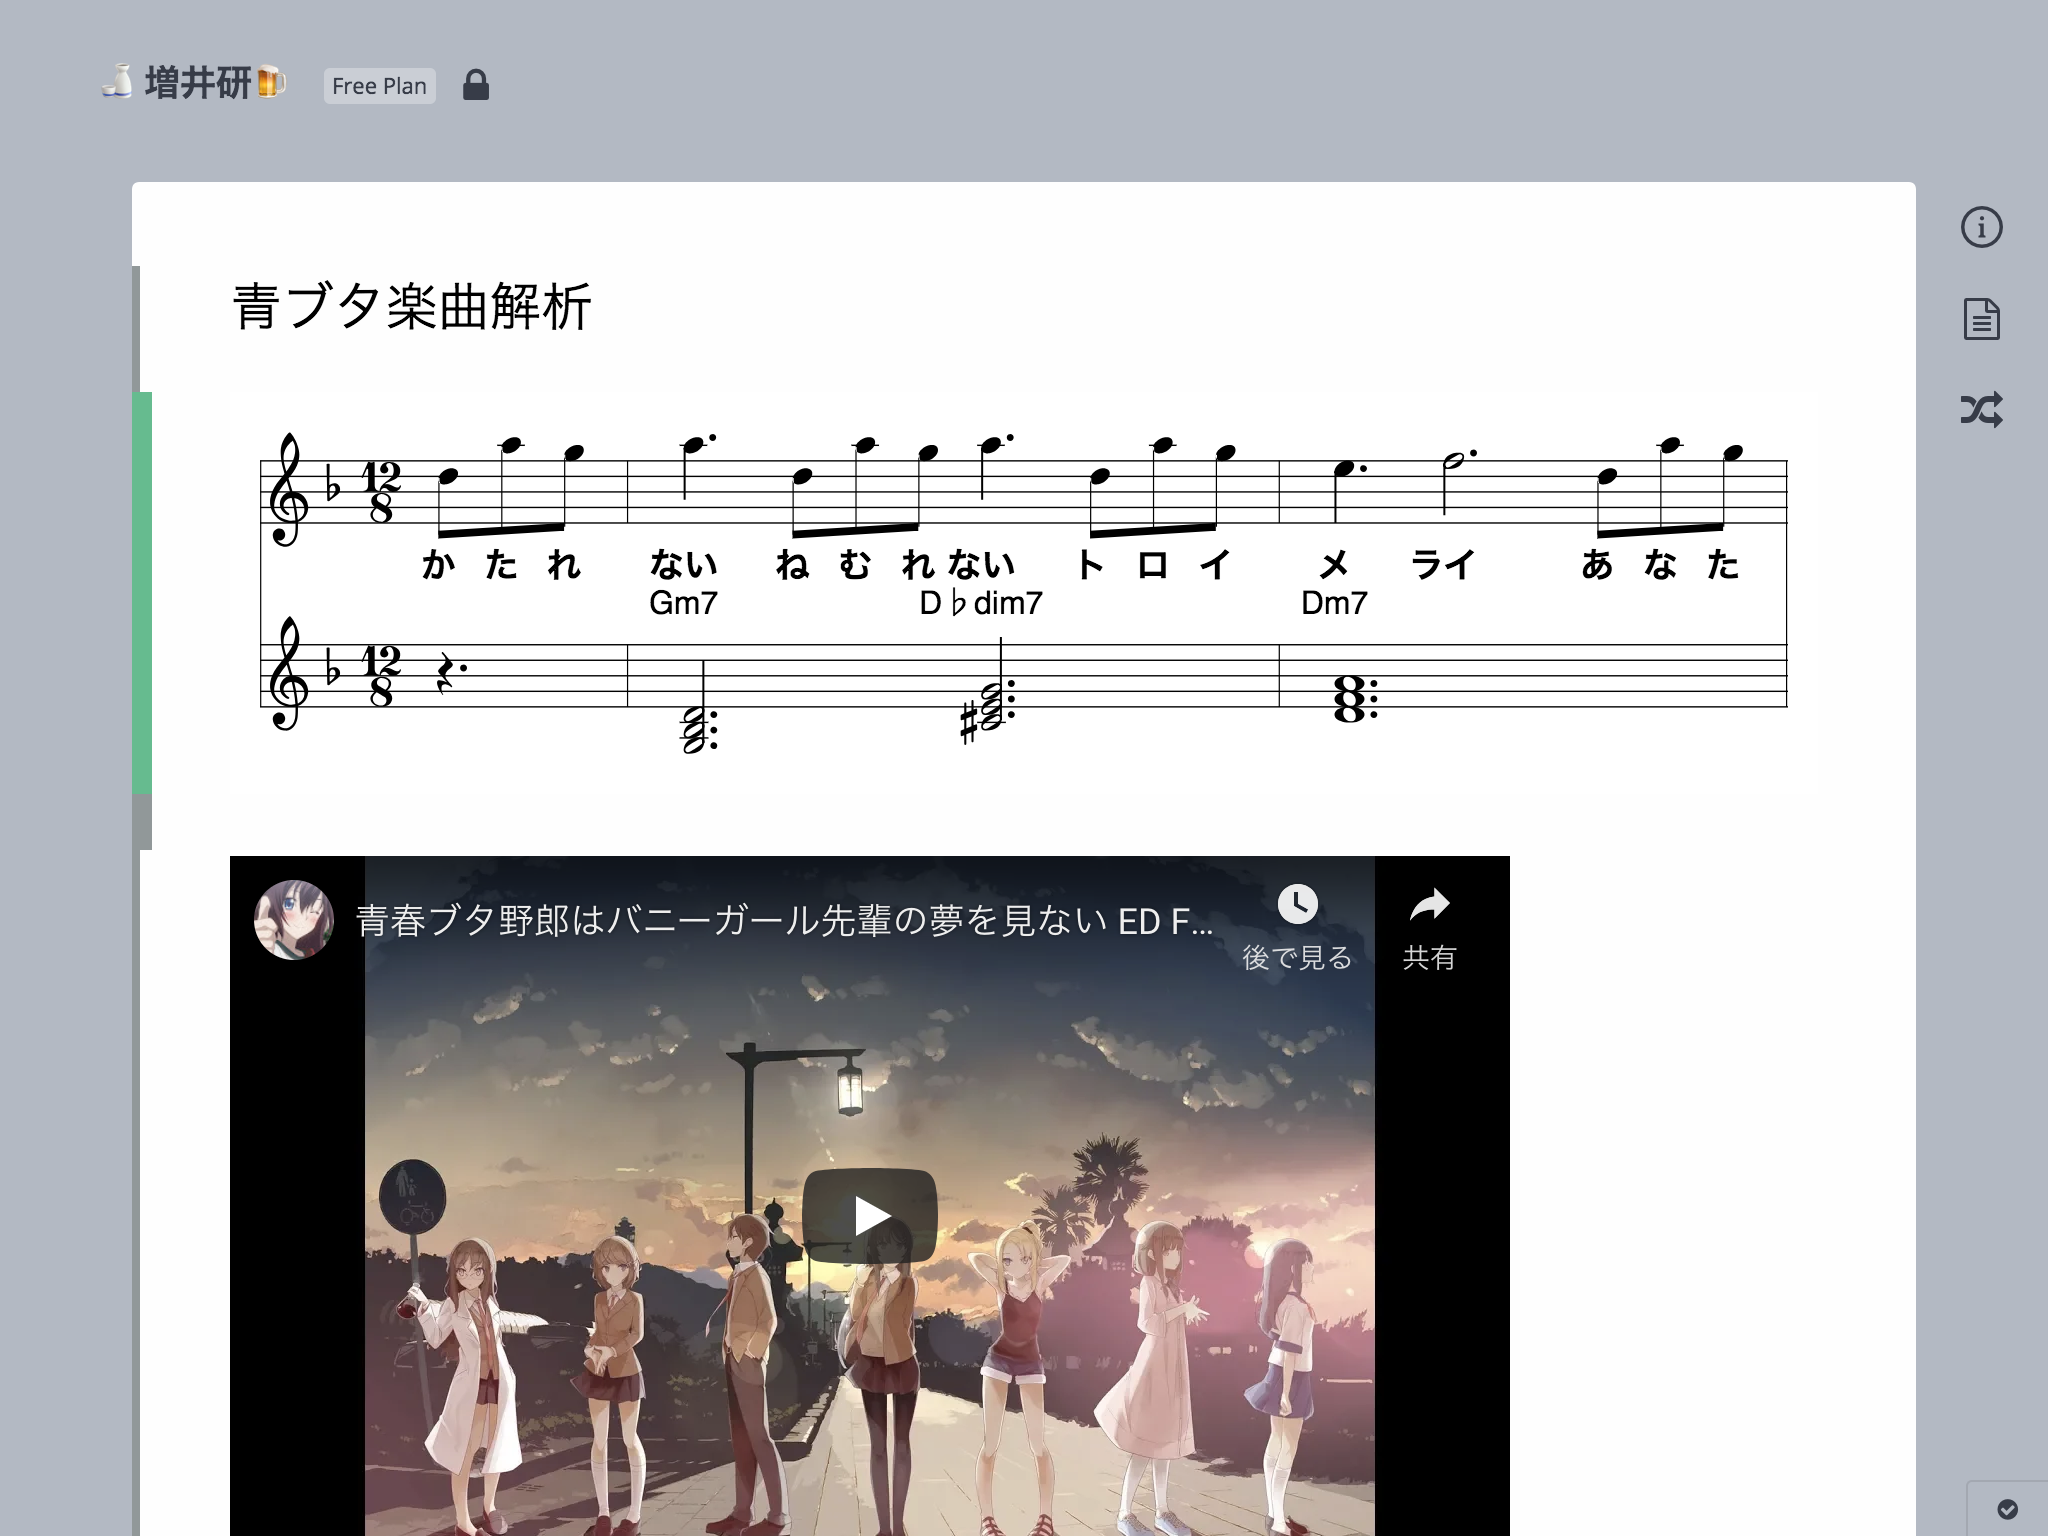
\includegraphics[width=10cm]{images/aobuta.png}
\caption{楽曲ページ}
\label{aobuta}
\end{figure}

\section{まとめ}
本章では、本システムによって実現可能な応用例について述べた。
Wikiと楽譜記述言語の組み合わせによって、今までにない新しい楽譜利用環境の実現が可能である。
本章で述べた応用例に限らず、様々な応用が可能と考えられる。
\chapter{関連研究}
\label{chap:kanren}

本章では楽譜関連研究を紹介し、それらの特徴や本研究との関連性について示す。

\newpage

\section{主要な研究領域}
楽譜に関連する主要な研究領域を紹介する。

\begin{enumerate}
  \item スコアアラインメント\\
  楽譜上のどの部分を演奏しているのか認識するためのスコアアラインメント技術が研究されている\cite{online}\cite{learning}\cite{coupled}\cite{automatic}。
  応用例として計算機による伴奏システム\cite{muens}\cite{mysong}、音楽鑑賞サポートシステム\cite{orchestra}、楽器練習サポートシステムなどが挙げられる\cite{tutor}。
  \item ジェスチャー楽譜入力インターフェース\\
  ジェスチャーを利用した楽譜入力インターフェースが提案されている\cite{notepad}\cite{pen}\cite{sssp}。
  これにより、計算機上でペンやポインティングデバイスを使って、楽譜を手書き入力することができる。
  \item 楽譜認識/再生システム\\
  画像から楽譜情報を読み取るための楽譜認識技術が研究されている\cite{optical}\cite{early}\cite{symbol}。
  これを応用して、カメラを搭載したデバイスによって印刷された楽譜を再生するシステムが提案されている\cite{onnote}\cite{gocen}。
\end{enumerate}

\section{楽譜編集/閲覧システム}
一般的に利用されている楽譜システムとは異なる、紙の楽譜の再現にとどまらない特徴を持った楽譜編集/閲覧システムを紹介する。

\subsection{BRASS}
Watanabeらが提案したBRASS\cite{Watanabe}(図\ref{brass})は、楽曲の全体構造を把握しながら楽譜を閲覧できるインタフェースによって、楽曲学習を支援する。
複数ページにまたがる規模の大きな楽譜では楽曲全体を把握するのが困難であるが、楽譜を圧縮表示し、音符の数やテンポの大小といったパラメータを濃淡や色によって可視化することで解決している。
ここで利用されている、空間を歪ませて注目部分を拡大表示する可視化手法はフォーカス+コンテクスト表示と呼ばれている。
本研究ではフォーカス+コンテクスト表示のような可視化の工夫は行っていないが、楽曲理解のために必要なテキスト/マルチメディアを自在に埋め込めることから、学習支援にも利用できる。

\begin{figure}[H]
\centering
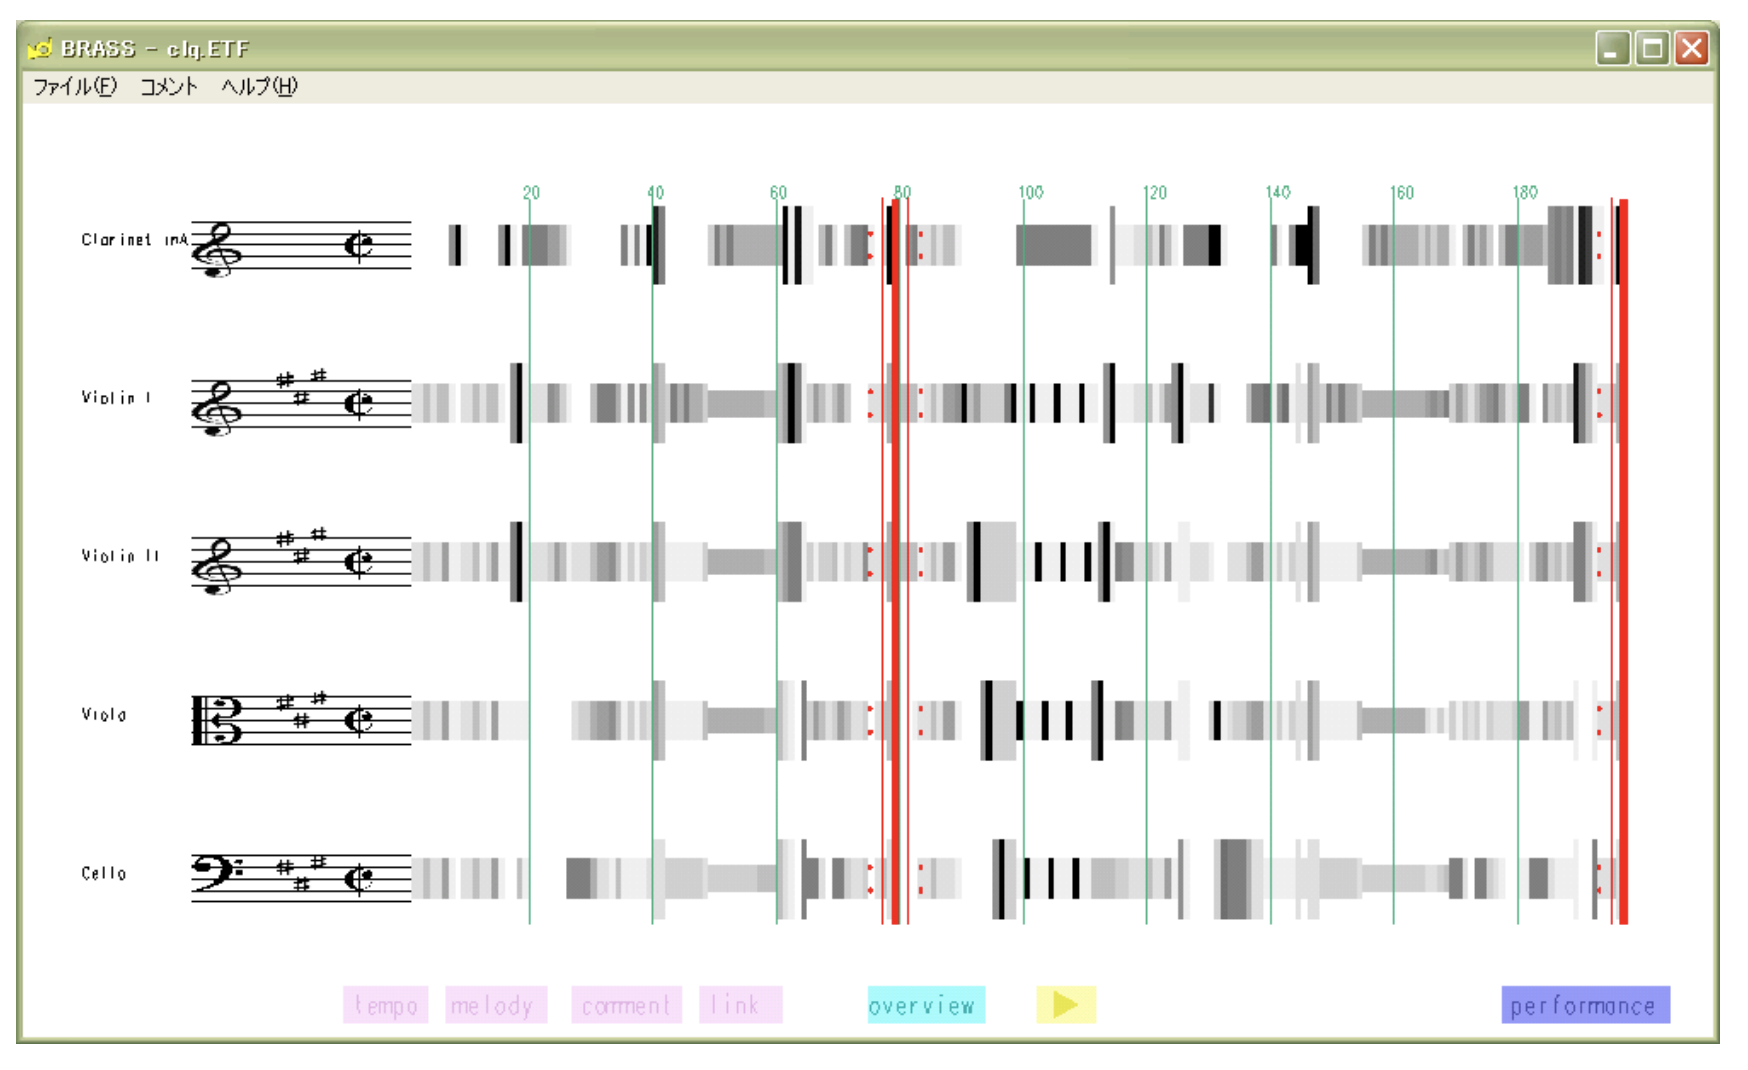
\includegraphics[width=10cm]{images/brass.png}
\caption{BRASSの画面}
\label{brass}
\end{figure}

\subsection{WIKI: :SCORE}
Almeidaらが提案したWIKI: :SCORE\cite{Almeida}(図\ref{wikiscore})は、Wiki上で楽譜の共同編集を行えるシステムである。
ABCによって楽譜を編集し、PDF/画像/音声といった各種フォーマット出力することができる。
複数パート/セクションを持つ規模の大きな楽譜の編集は大変な作業であるが、共同編集や楽譜の出力を行えることで、複数人で協力して実行することが可能である。
WikiとABCによるシステムであることからハイパー楽譜システムに設計が近いが、以下の点で異なっている。
\begin{itemize}
\item 共同編集のみを問題にしている
\item 編集環境がWYSIWYGでない
\item 楽譜専用のWikiである
\end{itemize}

\begin{figure}[H]
\centering
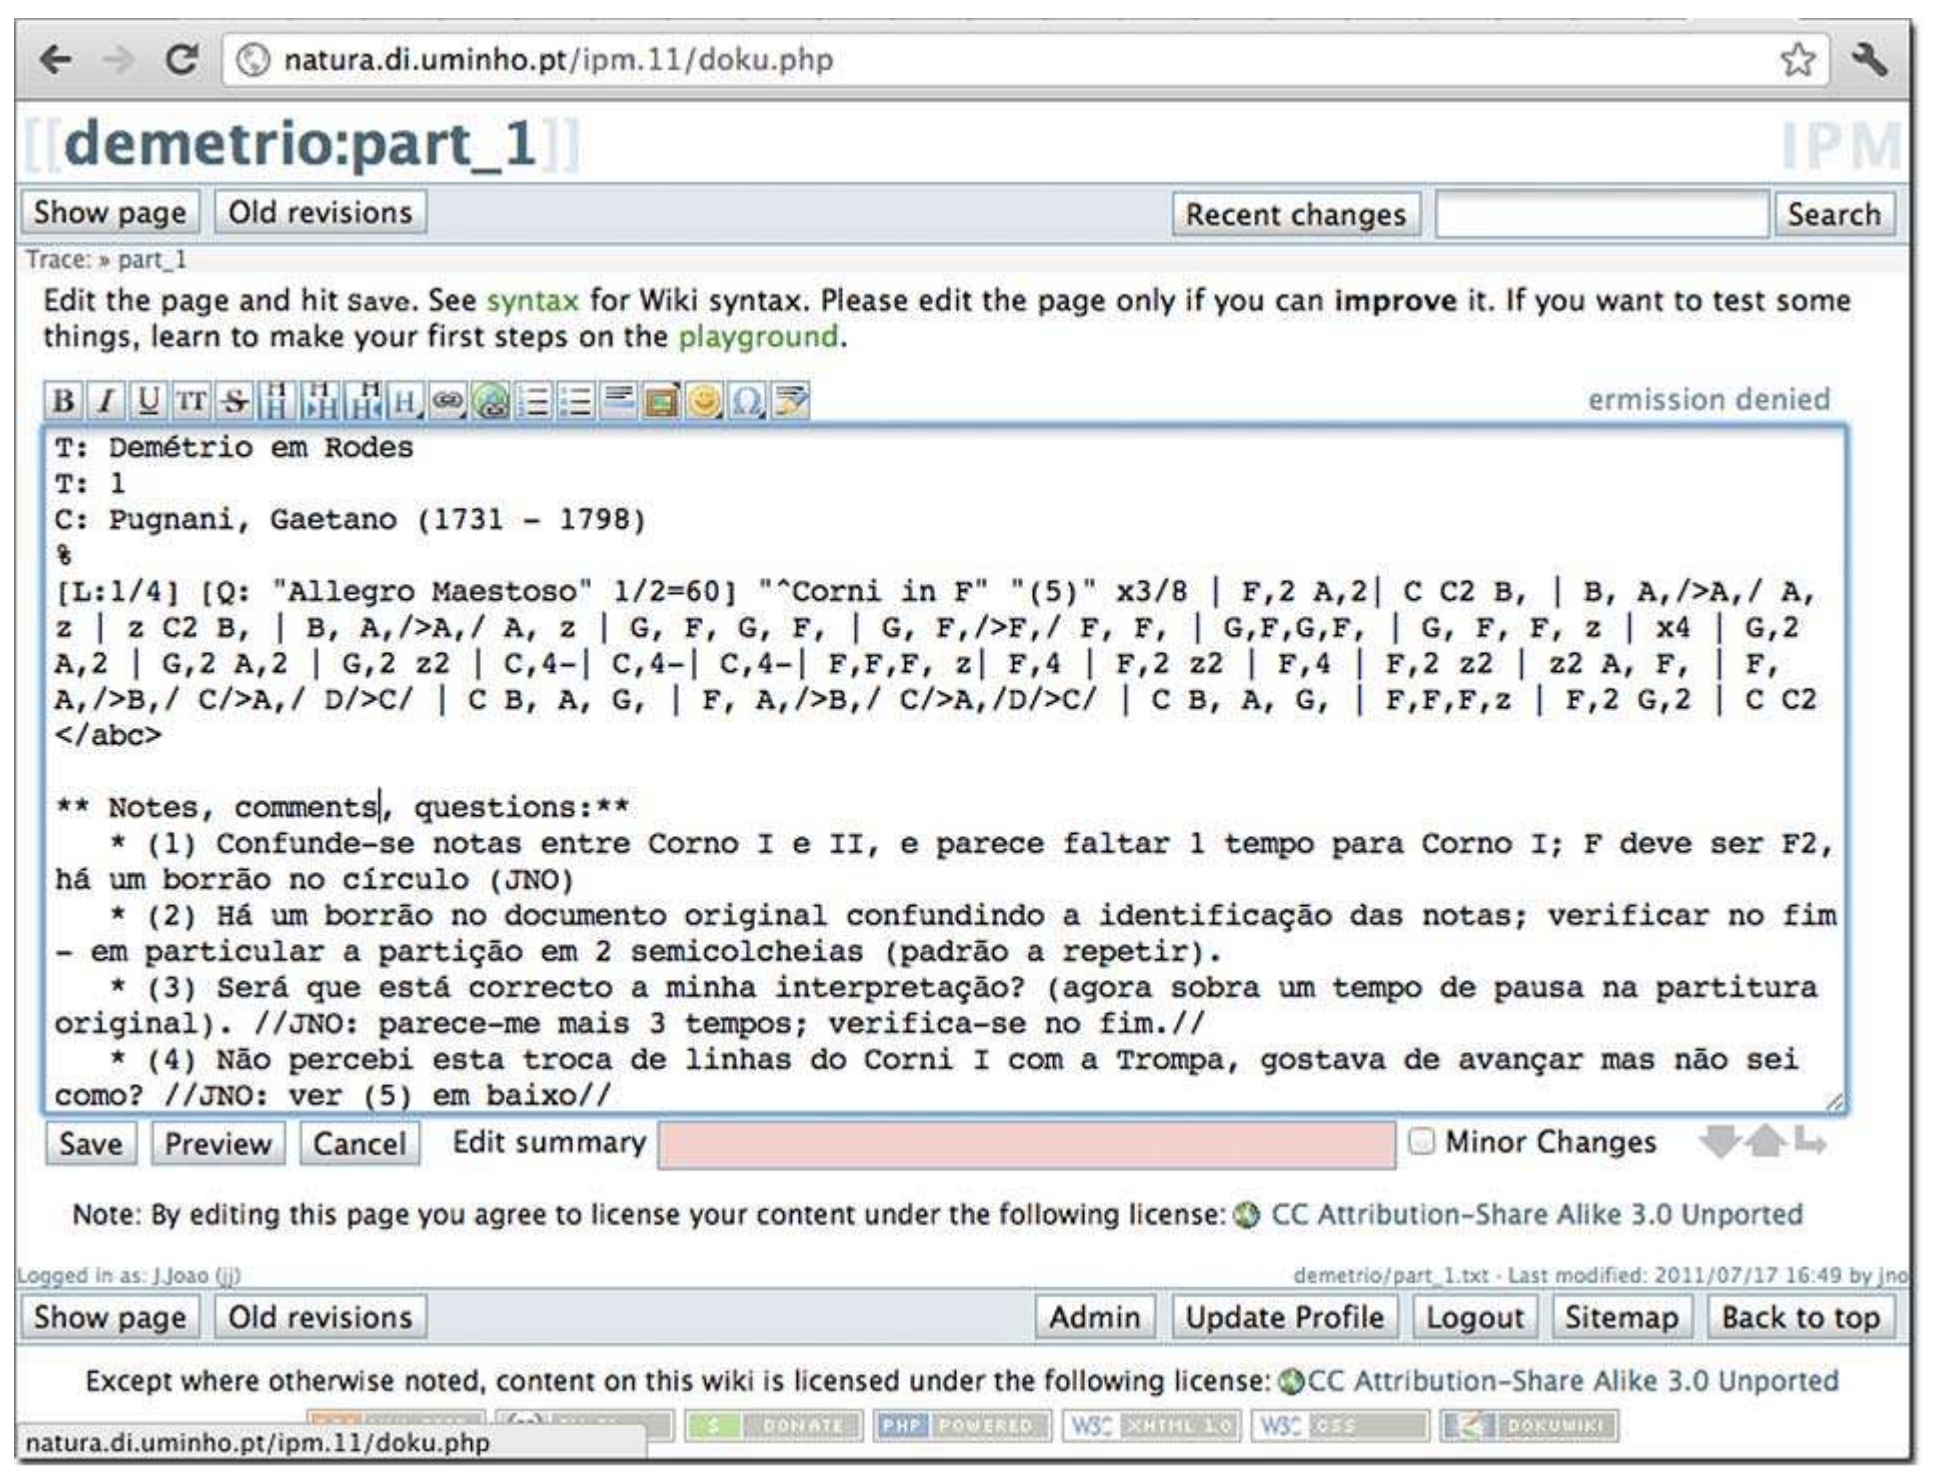
\includegraphics[width=10cm]{images/wikiscore.png}
\caption{WIKI: :SCOREの画面}
\label{wikiscore}
\end{figure}

\section{楽譜記述言語}
楽譜記述言語は楽譜をベースとした楽曲を記録・共有する目的で利用されており、本研究で利用しているABC記譜法もその1つである。
本節ではABC以外に広く利用されているものを解説する。
比較のために、図\ref{cdef}の楽譜を記述する各言語の例を示す。
ソースコード\ref{abcdef}はABCにおける記述例である。

\begin{figure}[H]
\centering
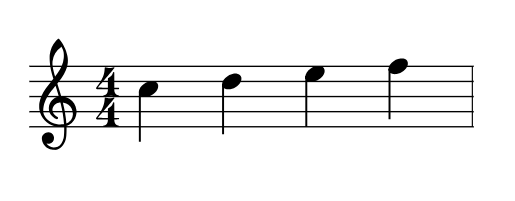
\includegraphics[width=5cm]{images/cdef.png}
\caption{「ドレミファ」の譜例}
\label{cdef}
\end{figure}

\begin{lstlisting}[caption=ABCにおける図\ref{cdef}の楽譜の記述例, label=abcdef]
M:4/4
L:1/4
cdef|
\end{lstlisting}

\subsection{MusicXML}
MusicXML\cite{XML}はXML形式の楽譜記述言語で、音符や小節といった音楽的要素が階層的に記述される。
各種楽譜作成ソフトでもMusicXMLによるインポート/エクスポートがサポートされており、楽譜データのやりとりに広く利用されている。
\begin{lstlisting}[caption=MusicXMLにおける図\ref{cdef}の楽譜の記述例(一部), label=xml]
<score-partwise>
  <part-list>
    <score-part id="P1">
      <part-name>Piano</part-name>
    </score-part>
  </part-list>
  <part id="P1">
    <measure number="1">
      <attributes>
        <divisions>1</divisions>
        <key>
          <fifths>0</fifths>
        </key>
        <time>
          <beats>4</beats>
          <beat-type>4</beat-type>
        </time>
        <clef>
          <sign>G</sign>
          <line>2</line>
        </clef>
      </attributes>
      <note>
        <pitch>
          <step>C</step>
          <octave>5</octave>
        </pitch>
        <duration>1</duration>
        <type>quarter</type>
      </note>
      <note>
        <pitch>
          <step>D</step>
          <octave>5</octave>
        </pitch>
        <duration>1</duration>
        <type>quarter</type>
      </note>
      <note>
        <pitch>
          <step>E</step>
          <octave>5</octave>
        </pitch>
        <duration>1</duration>
        <type>quarter</type>
      </note>
      <note>
        <pitch>
          <step>F</step>
          <octave>5</octave>
        </pitch>
        <duration>1</duration>
        <type>quarter</type>
      </note>
      <barline>
        <bar-style>light</bar-style>
      </barline>
    </measure>
  </part>
</score-partwise>
\end{lstlisting}

\subsection{Lilypond}
Lilypond\cite{Lily}はテキスト形式の楽譜記述言語および楽譜出力アプリケーションで、コマンドラインから利用できる。
印刷を意識した高度な楽譜作成が可能で、GUI楽譜作成ソフトで利用できるようなレイアウト調節パラメータを多く持つ。
\begin{lstlisting}[caption=Lilypondにおける図\ref{cdef}の楽譜の記述例, label=lily]
{
    \time 4/4
    c''4 d'' e'' f''
}
\end{lstlisting}

\subsection{VexTab}
VexTab\cite{Vex}はテキスト形式の楽譜記述言語および楽譜出力アプリケーションで、JavaScriptライブラリから利用できる。
HTML Canvas/SVGに楽譜を出力可能であり利用形態はABCに最も近いが、記法がやや冗長である。
\begin{lstlisting}[caption=VexTabにおける図\ref{cdef}の楽譜の記述例, label=vex]
stave
time=4/4
notes :4 C/5D/5E/5F/5|
\end{lstlisting}


\chapter{考察}
\label{chap:kosatsu}

本章では、ハイパー楽譜システム利用者の意見や自身の運用経験をまとめ、諸問題や新しい可能性について述べる。

\newpage

\section{評価}
本システムのプロトタイプとなるChrome拡張機能「hyperscorebox」を2018年11月21日にChrome Web Storeで公開した\footnote{\textsf{https://chrome.google.com/webstore/detail/hyperscorebox/cjlhoobllhkpjjomlijlfdblgifcdmoh}}。2018年12月現在、60名程度にインストールされている。
また、Web技術や音楽アプリ関連情報を共有する以下の開発者イベントにて hyperscorebox の展示発表を行った。
\begin{itemize}
    \item WebAudio.tokyo \#6\footnote{\textsf{https://webaudiotokyo.connpass.com/event/103821/}} (2018年11月15日 株式会社ドリコム)
    \item HTML5 Conference 2018\footnote{\textsf{https://events.html5j.org/conference/2018/11/}} (2018年11月25日 電気通信大学)
    \item Web Music Developers Meetup \#3\footnote{\textsf{https://connpass.com/event/112300/}} (2018年12月21日 株式会社デジタルハーツ)
\end{itemize}
本節では、
\begin{itemize}
    \item 筆者の運用経験
    \item ユーザーからのフィードバック
    \item 各種展示発表でのフィードバック
\end{itemize}
をまとめる。

\subsection{筆者の運用経験}
主に楽器練習/音楽理論の勉強/採譜といった用途で3ヶ月に渡り利用した。
\paragraph*{楽器練習}
筆者はクラシックギターの練習に本システムを利用しており、練習中に残した様々なメモを整理して記録できている。
以前まではたくさん書き込んでも練習する曲それぞれの楽譜に散逸してしまうため整理や再利用が難しく、結局役に立たないという問題に悩まされていたが、本システムによって解決された。
\paragraph*{音楽理論の勉強}
既存の教材に強く苦手意識を抱いていたが、自身が演奏している楽曲と知識の関係性がハイパーリンクによって可視化され、自分専用の分かりやすい教材として利用できている。
また音声の埋め込みによって実際の演奏を聞きながら学習でき、イメージしづらい概念の理解を深めるのに特に有効である。
\paragraph*{採譜}
筆者は本システムの利用前までABCの利用経験が無かったが、複雑な楽譜でない限りは楽譜IMEの支援によって快適に楽譜編集できている。
また採譜した楽曲の音声/動画/作曲者/演奏者といった周辺情報を一元管理でき便利である。

\subsection{感想・意見}
まず、第\ref{mondai}節で述べた楽譜の問題点に対して多くの賛同を得られた。
多くのユーザーは楽譜に不便さを感じていたものの、根本的な解決手段を見つけられない状況に置かれている。
その他の感想や意見として主に以下のようなものが挙げられた。

\begin{enumerate}
    \item 楽譜やコメントを瞬時に共有できる\\
    楽譜や演奏に対する要望を伝えるには「3小節目の1拍裏のドの音を半音上げて」「100小節のシドレミのフレーズをもっと大きく」といった具体的な指示を行う必要がある。
    本システムでは楽譜と一緒にコメントを書いたり、その場で楽譜を更新して瞬時に共有できるので、コミュニケーションコストを大幅に小さくできるのではないかという好意的な評価を得た。
    \item 既存の楽譜作成システムを使うには大げさなシーンで価値がある\\
    既存の楽譜作成システムを使って1.のような楽譜共有を実現する場合、
    \begin{enumerate}
        \item ソフトを起動して楽譜入力する
        \item スクリーンショットを撮影する
        \item 画像をSNS等で送信する
    \end{enumerate}という作業が必要である。
    そもそも楽譜作成システムは断片的な楽譜の作成を前提としていないため、楽譜そのものとは関係ないレイアウトや設定を意識する必要があり、このような用途では大袈裟である。
    一方本システムでは素早く書けてすぐ共有できるため好評であった。
    \item Webリソースを活用できる\\
    紙やPDF上の楽譜は静的で独立したメディアなので、外部の情報を活用したりリンクすることができない。
    マルチメディア情報をはじめとするWeb上の様々なリソースを活用しながら楽譜編集するという応用は新鮮なものとして受け止められ、大きな可能性を感じられるという感想を得た。
\end{enumerate}

\subsection{問題点}
問題点として以下のようなものが挙げられた。
\begin{enumerate}
    \item リンク機能について\\
    複数の音符にハイパーリンクが設定されている場合、すべての音符が1つのリンクを示しているのか、それぞれの音符が別のリンクを示しているのか一目見て理解できないという意見が挙げられた。
    これはリンク先にかかわらず全て青色の音符として表示しているためであるが、単音に対しても、フレーズや小節に対してもリンクを設定したいので、何らかのインタフェース的工夫が必要である。
    \item 楽譜編集について\\
    既存の楽譜を取り込めるような仕組みがほしいという意見が挙げられた。
    楽譜を自ら編集することを前提としているため、既存の楽曲を利用したい場合は元になる楽譜を別途用意したり、採譜したりして自分で入力する必要がある。
    楽譜IMEによってある程度入力作業が簡単になるものの、すぐ楽譜を利用したいユーザーにとっては大きな負担になる。
    \item 利用環境について\\
    タブレット上でも快適に本システムを利用したいという意見が挙げられた。
    PCブラウザ上での利用を前提とした設計のため、タブレットのようなタッチインタフェース端末では利用しづらい。
    既存の楽譜ビューアーはタブレットで利用されるものがほとんどであり、譜面台の上のような限られたスペースでも快適に利用できるため好まれている。
\end{enumerate}

\section{考察}
\subsection{設計の妥当性}
本システムは既存のものとは全く異なる新しい楽譜の利用形態を持つが、実際に利用したりデモを体験したユーザーからは概ね好意的に受け入れられ、Wikiと楽譜記述言語を組み合わせるという本システムの設計指針は正しかったといえる。
また本研究で述べた楽譜に対する問題意識にも多くの共感を得られたことから、本システムをベースにして様々な改善や拡張を行うことで、より良い楽譜利用環境を生み出せると考えられる。
\subsection{解決すべき課題}
\begin{enumerate}
    \item 音符のリンク状況が分からない\\
    音符にリンクが設定されている場合、リンク先を把握するにはABCを確認するか、実際に音符をクリックする必要があり非効率である。
    Webブラウザではフォーカスされたリンクに下線を付けたり、画面左下にリンク先アドレスを表示することで解決している。
    本システムでも同様の手法が有効であると考えられる。
    \item 自分で楽譜を書く必要がある\\
    IMSLP\footnote{\textsf{https://imslp.org}}といったパブリックドメイン楽譜配布サイトや出版社による販売サイト上には膨大な数の楽譜が存在し、ユーザーは必要とする楽譜をWebから簡単に見つけ出すことができるため、通常自ら楽譜を書く必要はない。
    本システムでも必要な楽譜をすぐ利用できるようにするために、既存の楽譜ファイルからABCへコンバートできる機能や、ユーザーが楽譜を配布できるWiki上のプラットフォームが必要であると考えられる。
    \item タブレットで使いづらい\\
    楽譜利用環境として主流であるタブレット上でも快適に利用できるようにするために、タッチインターフェースに適した以下のようなインタフェースの工夫が必要であると考えられる。
    \begin{itemize}
        \item ボタン/ペン操作による楽譜入力
        \item ハンズフリーな楽譜スクロール
    \end{itemize}
\end{enumerate}

\subsection{楽譜の問題点の検証}
本システムにおいて第\ref{mondai}節で述べた問題点が克服されているかどうかを問題点毎に検証する。
\begin{itemize}
    \item 簡単に編集できない\\
    新規作成/既存楽譜の編集両方を、楽譜IMEの支援を受けながら簡単に行える。
    \item メモなどの情報を自在に書けない\\
    楽譜と同じ場所にテキスト/マルチメディア情報を自在に書ける。
    \item 参照や管理が面倒\\
    楽譜内のハイパーリンクによって関連する楽譜や情報を辿って参照できる。
\end{itemize}
以上のように、第\ref{mondai}節で述べたすべての点に関して問題が解決していることがわかる。
\chapter{結論}
\label{chap:kekka}

本章では本研究を総括する。

\newpage

\section{研究の成果}
本研究では、Wikiと楽譜記述言語を組み合わせた新しい楽譜システム「ハイパー楽譜システム」と、日本語入力システム的アプローチによる楽譜入力支援システム「楽譜IME」の提案を行った。

まず第\ref{chap:haikei}章において、楽譜の問題点をテキストの進化と比較しながら分析した。楽譜を扱う既存システムの現状をとりあげ、計算機が普及した現在も根本的に解決されていないことを示した。

第\ref{chap:sekkei}章では、第\ref{chap:haikei}章で述べた楽譜の問題点に対する有効的な解決方法を提案した。また、それに基づき本研究で開発した「ハイパー楽譜システム」の基本構成と使い方について述べた。

第\ref{chap:jissou}章では、「ハイパー楽譜システム」のアプリケーション構成と詳細な実装について述べた。

第\ref{chap:ime}章では、テキストによる楽譜入力には限界があることを示し、日本語入力システム的アプローチによる楽譜入力支援システム「楽譜IME」を提案した。

第\ref{chap:ouyou}章では、「ハイパー楽譜システム」によって実現可能な応用例について述べた。

第\ref{chap:kanren}章では、本研究に関連する研究を紹介し、それぞれのアプローチの特徴と問題点を分析した。

第\ref{chap:kosatsu}章では、筆者による運用経験やユーザーからのフィードバックをもとに本研究の有効性と問題点を分析した。

\section{総括}
本研究では楽譜を簡単に書いたり音符など以外の情報を自在に書いたりハイパーリンクを利用できる「ハイパー楽譜システム」とABCの入力を支援する「楽譜IME」の開発を行った。
ハイパー楽譜システムはWikiと楽譜記述言語の組み合わせによって既存の楽譜の問題点を克服するだけでなく、新しい楽譜の使い方を実現した。
楽譜IMEは日本語入力システムのアプローチを取ることでテキストによる楽譜入力の弱点を克服し、既存の楽譜作成システムに劣らない快適な楽譜入力を可能にした。
今後は第\ref{chap:kosatsu}章で述べた問題点についての改善や、システムの拡張を行っていく。

\begin{acknowledgment}

学部から5年間の長きに渡りご指導を賜りました慶應義塾大学環境情報学部 増井俊之教授に深く感謝いたします。また、本研究の副査としてご意見、ご助言を頂きました小川克彦教授、中西泰人教授に感謝いたします。

学部・修士の4年間を共に過ごし、自身の研究について幅広い議論をしていただいた政策・メディア研究科修士課程の早川匠氏、様々な形でアドバイスをくださった増井俊之研究会OB諸氏に感謝いたします。

\end{acknowledgment}
  % 謝辞。要独自コマンド、include先参照のこと

\begin{bib}[100]
\bibliography{main}
\end{bib}
  % 参考文献。要独自コマンド、include先参照のこと
\appendix

\end{document}
